\part{P、QRS、T、U各波段正常值及其异常改变}

本篇根据心电图波形产生的顺序着重讨论了各波段的心电图改变及其临床意义,包括窦性P波及其异常改变、异位P波、房性融合波、心房内差异性传导、PR段偏移及P-R间期异常与P-J间期、正常QRS波群及其异常改变、与心源性猝死相关的波(J波、Epsilon波、Brugada波及Lambda波)、正常ST段及其异常改变、正常T波及其异常改变、正常Q-T间期及其异常改变、正常U波及其异常改变,共8章。

\protect\hypertarget{text00007.html}{}{}

\protect\hypertarget{text00007.htmlux5cux23chapter7}{}{}

\chapter{窦性P波、异位P波及其异常改变}

\protect\hypertarget{text00007.htmlux5cux23subid1}{}{}

\section{窦性P波及其异常改变}

\protect\hypertarget{text00007.htmlux5cux23subid2}{}{}

\subsection{正常窦性P波}

1.心电图特征

(1)P波极性:在Ⅰ、Ⅱ导联直立,aVR导联倒置,V\textsubscript{1}
导联呈正、负双相或直立,V\textsubscript{5} 、V\textsubscript{6}
导联直立。

(2)P波时间:各导联P波时间<0.11s,两切迹的峰距<0.04s。

(3)P波振幅:Ⅱ、Ⅲ、aVF导联P波振幅<0.25mV或低电压时,其P波振幅小于同导联R波振幅的$\frac{1}{2}$
,V\textsubscript{1} 导联P波正相波的振幅<0.15mV,V\textsubscript{5}
导联P波振幅<0.2mV。

(4)V\textsubscript{1} Ptf值:又称为V\textsubscript{1}
导联P波负相终末电势,正常值<|-0.04mm·s|。

(5)P-P间期互差<0.16s。

2.形成机制

窦性冲动优先地通过前、中结间束等心房内传导组织使心房肌除极产生P波,其除极方向从右前上向左后下除极,所形成的P波前$\frac{1}{3}$
为右心房除极,后$\frac{1}{3}$
为左心房除极,中$\frac{1}{3}$
为左、右心房及房间隔同时除极。

\protect\hypertarget{text00007.htmlux5cux23subid3}{}{}

\subsection{电轴左偏型P波}

1.心电图特征

(1)Ⅰ、aVL导联P波直立,其振幅大于Ⅱ导联的P波。

(2)Ⅱ导联P波低平或正、负双相,Ⅲ、aVF导联P波呈正、负双相(Ⅲ导联P波可浅倒)。

(3)aVR导联P波浅倒或负、正双相。

(4)P波时间、振幅多正常。

(5)起卧活动后,Ⅱ、Ⅲ、aVF导联P波振幅明显增高。这反过来可证实电轴左偏型P波与起搏点起源于窦房结尾部有关(图\ref{fig1-1})。

\begin{figure}[!htbp]
 \centering
 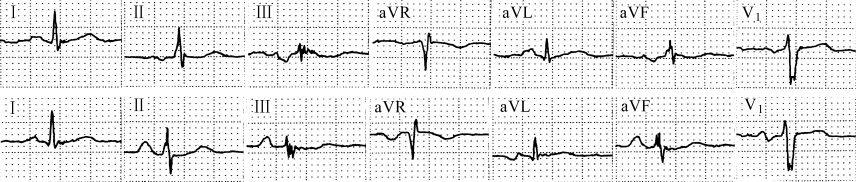
\includegraphics[width=5.78125in,height=1.22917in]{./images/Image00006.jpg}
 \captionsetup{justification=centering}
 \caption{健康体检者出现P波电轴左偏(下行系活动后记录)}
 \label{fig1-1}
  \end{figure} 

2.发生机制

(1)与窦房结起搏点的位置改变有关:窦房结头部的自律性较尾部高,且头部的冲动优先地通过前结间束下传心房,所形成的P波电轴多在+15°~+75°,故Ⅱ、Ⅲ、aVF导联P波振幅最高。而尾部发放的冲动优先地通过中结间束下传心房,所形成的P波电轴多在+15°~-30°,此时Ⅰ、aVL导联P波振幅高于Ⅱ导联。

(2)与心脏在胸腔的位置改变有关:当心脏在胸腔内发生顺钟向或逆钟向转位时,会影响心房除极所产生的P向量环的位置(正常P向量环位于左后下),进而影响各个导联P波的振幅甚至极性。

3.鉴别诊断

主要与房性异位心律相鉴别。若P波在Ⅰ、aVL导联直立,Ⅱ、aVF导联呈负、正双相,Ⅲ导联浅倒,aVR导联呈正、负双相,则为房性异位心律。

\protect\hypertarget{text00007.htmlux5cux23subid4}{}{}

\subsection{二尖瓣型P波}

因该P波常见于风心病二尖瓣狭窄患者,故称为“二尖瓣型P波”。

1.心电图特征

(1)P波时间≥0.11s,呈双峰切迹,两峰距≥0.04s,多出现在Ⅱ、Ⅲ、aVF、V\textsubscript{3}
~V\textsubscript{6}
等导联;若伴有P波电轴左偏,则出现在Ⅰ、aVL、V\textsubscript{5} 等导联。

(2)V\textsubscript{1}
Ptf值≥|-0.04mm·s|(多见于风心病二尖瓣狭窄患者)。

(3)P波振幅正常(图\ref{fig1-2})。

\begin{figure}[!htbp]
 \centering
 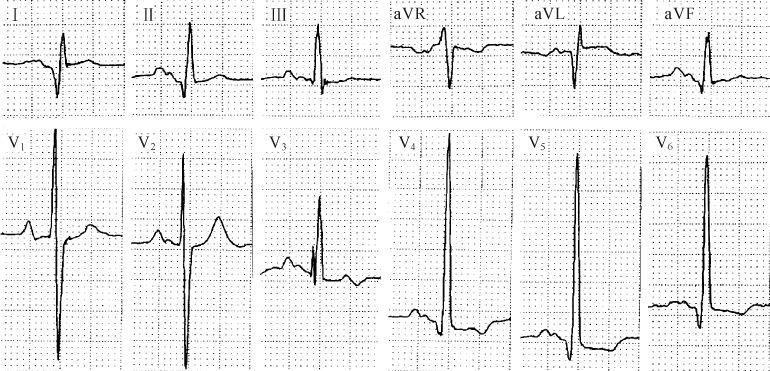
\includegraphics[width=5.19792in,height=2.5in]{./images/Image00007.jpg}
 \captionsetup{justification=centering}
 \caption{风心病、二尖瓣狭窄伴关闭不全患者,出现二尖瓣型P波及V\textsubscript{1}}
 \label{fig1-2}
  \end{figure} 
导联P波高尖(提示双心房肥大)、高侧壁及前侧壁异常Q波、左右胸前导联QRS波群高电压(提示双心室肥大)、前侧壁ST-T改变

2.发生机制

当左心房扩大、肥大或房间束(Bachmann束)、左心房内传导功能减低时,将导致左心房除极时间延长,从而使整个心房的除极时间也相应地延长。

3.临床意义

(1)左心房负荷过重:主要见于早期风心病二尖瓣狭窄、左心房黏液瘤、急性左心衰竭等。

(2)左心房扩大或肥大:凡是能导致左心房负荷持续加重的病因,均可引起左心房扩大或肥大。主要见于风心病二尖瓣狭窄,也见于扩张型心肌病、高血压性心脏病等。

(3)不完全性左心房内传导阻滞或房间束(Bachmann束)传导阻滞:多见于冠心病、心肌梗死、心肌炎及低钾血症等。

(4)左心房扩大合并左心房内传导阻滞:左心房扩大易损伤心房内传导组织,引起心房内传导阻滞,导致P波时间明显增宽(>0.14s)。

(5)易发生各种房性心律失常:左心房负荷长期过重,导致左心房扩大或肥大,继而牵拉和损伤心房内传导组织,引起心房内异位起搏点自律性增高、折返现象或触发活动,诱发多源性房性早搏、短阵性房性心动过速、心房扑动或心房颤动等。

\protect\hypertarget{text00007.htmlux5cux23subid5}{}{}

\subsection{肺型P波}

因该P波常见于慢性肺心病患者,故称为“肺型P波”。

1.心电图特征

(1)P波形态高尖:在Ⅱ、Ⅲ、aVF导联P波振幅≥0.25mV,V\textsubscript{1}
、V\textsubscript{2} 导联P波振幅≥0.15mV。

(2)低电压时,P波振幅≥同导联R波振幅的$\frac{1}{2}$
。

(3)P波时间多正常。

(4)部分患者V\textsubscript{1}
Ptf值≥|-0.04mm·s|,但V\textsubscript{1}
导联P波负相波表现为深而窄(图\ref{fig1-3})。

\begin{figure}[!htbp]
 \centering
 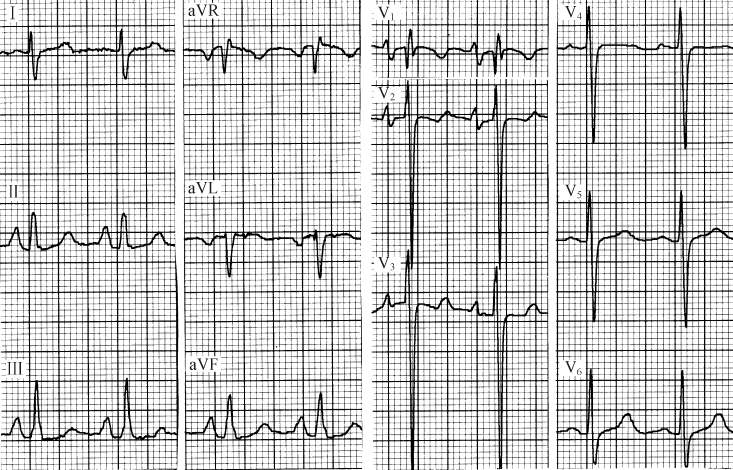
\includegraphics[width=4.94792in,height=3.17708in]{./images/Image00008.jpg}
 \captionsetup{justification=centering}
 \caption{慢性支气管炎、肺心病患者出现肺型P波、V\textsubscript{1}}
 \label{fig1-3}
  \end{figure} 
Ptf值增大及右心室肥大(V\textsubscript{4} ~V\textsubscript{6}
导联定准电压0.5mV)

2.发生机制

因右心房除极比左心房早,且较早结束除极,故右心房扩大、肥大或右心房内传导功能减低时,其除极时间虽然有所延长,但大多不至于延长到左心房除极结束之后。因此,整个心房除极时间并不延长,但因其除极时所产生的向右前向量增大,故出现P波高尖。

3.临床意义

(1)右心房负荷过重:见于急性右心衰竭、早期肺动脉高压、甲状腺功能亢进、急性支气管炎、肺部炎症及长期吸烟者等。

(2)右心房扩大或肥大:凡是能导致右心房负荷持续加重的病因,均可引起右心房扩大或肥大。主要见于肺心病、先心病(如法洛四联症、房间隔缺损等)等。

(3)不完全性右心房内传导阻滞:多见于冠心病、心肌梗死、心肌炎及低钾血症等。

(4)右心房扩大合并右心房内传导阻滞。

(5)颅内血肿、肿瘤亦可出现肺型P波。

(6)交感神经兴奋性增高。

(7)易发生各种房性心律失常,如多源性房性早搏、短阵性房性心动过速、心房扑动或心房颤动等。

\protect\hypertarget{text00007.htmlux5cux23subid6}{}{}

\subsection{先心型P波}

因该P波常见于先心病患者,故称为“先心P波”。

1.心电图特征

(1)P波形态高尖:在Ⅱ、Ⅲ、aVF导联P波振幅≥0.25mV,V\textsubscript{1}
、V\textsubscript{2} 导联P波振幅≥0.15mV,V\textsubscript{5}
导联P波振幅≥0.2mV(图\ref{fig1-4})。

\begin{figure}[!htbp]
 \centering
 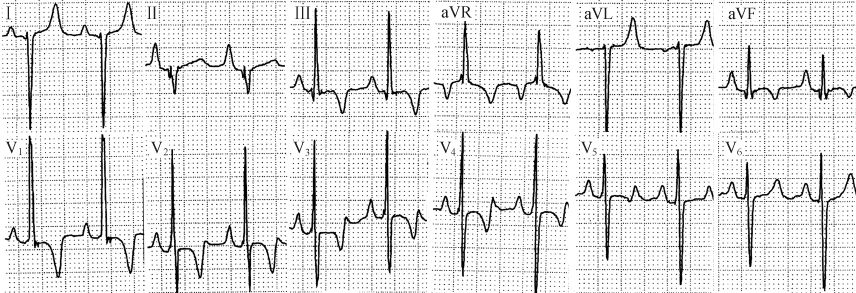
\includegraphics[width=5.78125in,height=1.97917in]{./images/Image00009.jpg}
 \captionsetup{justification=centering}
 \caption{先心病、法洛四联症患者,出现右心房、右心室肥大}
 \label{fig1-4}
  \end{figure} 

(2)P波时间多正常,但右心房显著扩大者,其除极时间将会明显延长,甚至延长至左心房除极结束之后,此时P波时间可≥0.12s。

2.临床意义

(1)右心房负荷过重。

(2)右心房扩大或肥大。

(3)易发生各种房性心律失常。

(4)当P波时间≥0.12s时,易误诊为双心房肥大。

\protect\hypertarget{text00007.htmlux5cux23subid7}{}{}

\subsection{交感型P波}

交感神经兴奋时,如运动、紧张等因素引起心率显著增快,可使原正常的P波,其振幅明显增高,出现类似“肺型P波”特点,称为交感型P波。系交感神经兴奋引起心房肌除极速度加快,导致右、左心房除极同步化,两者同时除极的部分叠加后使P波振幅明显增高。心率减慢后,P波形态、振幅均恢复正常(图\ref{fig1-5})。

\begin{figure}[!htbp]
 \centering
 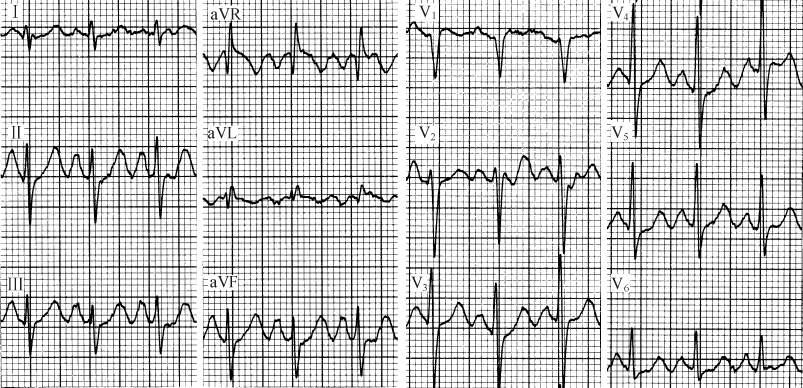
\includegraphics[width=5.42708in,height=2.61458in]{./images/Image00010.jpg}
 \captionsetup{justification=centering}
 \caption{平板运动试验患者出现窦性心动过速、交感型P波、假性电轴左偏(-90°)}
 \label{fig1-5}
  \end{figure} 

\protect\hypertarget{text00007.htmlux5cux23subid8}{}{}

\subsection{巨大型P波}

凡是P波时间≥0.11s、振幅≥0.25mV者,称为巨大型P波。

1.心电图特征

(1)P波振幅增高:在Ⅱ、Ⅲ、aVF导联P波振幅≥0.25mV,V\textsubscript{1}
、V\textsubscript{2} 导联P波振幅≥0.15mV。

(2)P波时间增宽:P波时间≥0.11s,呈双峰切迹,两峰距≥0.04s,一般在Ⅰ、Ⅱ、aVF、V\textsubscript{3}
~V\textsubscript{6} 导联增宽最明显。

(3)V\textsubscript{1} Ptf值多≥|-0.04mm·s|(图\ref{fig1-6})。

\begin{figure}[!htbp]
 \centering
 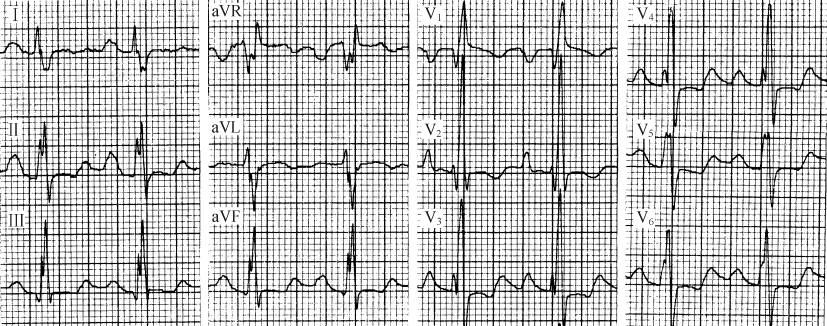
\includegraphics[width=5.58333in,height=2.19792in]{./images/Image00011.jpg}
 \captionsetup{justification=centering}
 \caption{先心病、房间隔缺损、二尖瓣狭窄患者出现巨大型P波(提示双心房肥大)、完全性右束支传导阻滞、前侧壁轻度ST段改变}
 \label{fig1-6}
  \end{figure} 

2.临床意义

(1)双心房负荷过重:严重的先心病患者,开始有左向右分流;当肺动脉压力大于左心室压力时,则出现右向左分流,引起左、右心房负荷过重。

(2)双心房扩大或肥大:左、右心房负荷持续过重,势必引起左、右心房扩大或肥大。见于风心病二尖瓣狭窄或伴关闭不全、扩张型心肌病及先心病(如室间隔缺损、动脉导管未闭)等。

(3)右心房扩大合并左心房内传导阻滞。

(4)左心房扩大合并右心房内传导阻滞。

(5)不完全性左、右心房内传导阻滞。

(6)右心房显著扩大:当右心房显著扩大时,右心房除极时间明显延长,甚至延长至左心房除极结束后,表现为P波振幅增高及时间增宽,酷似双心房扩大。见于严重的肺动脉高压、Ebstein畸形(先天性三尖瓣下移综合征)的部分患者。

(7)易发生各种房性心律失常。

\protect\hypertarget{text00007.htmlux5cux23subid9}{}{}

\subsection{间歇性P波改变}

窦性心律时,其P波形态、振幅呈间歇性改变,见于间歇性心房内传导阻滞、P波电交替、窦房结头部与尾部交替性或间歇性发放冲动等。

(1)间歇性心房内传导阻滞:在P-P间期基本规则时,间歇性出现正常P波、肺型P波或(和)二尖瓣型P波(图\ref{fig1-7}、图\ref{fig1-8})。

\begin{figure}[!htbp]
 \centering
 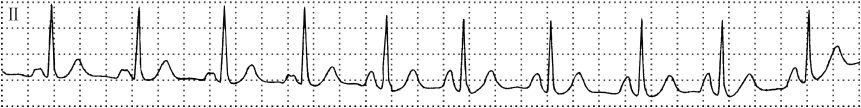
\includegraphics[width=5.82292in,height=0.72917in]{./images/Image00012.jpg}
 \captionsetup{justification=centering}
 \caption{风心病、二尖瓣狭窄患者出现二尖瓣型P波(左心房肥大所致)和肺型P波(间歇性右心房内传导阻滞所致)}
 \label{fig1-7}
  \end{figure} 

\begin{figure}[!htbp]
 \centering
 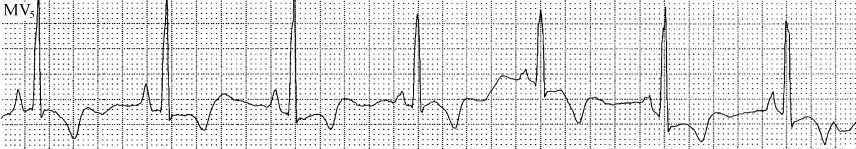
\includegraphics[width=5.78125in,height=1in]{./images/Image00013.jpg}
 \captionsetup{justification=centering}
 \caption{冠心病患者间歇性出现不完全性右心房内传导阻滞引起一过性肺型P波、ST-T改变}
 \label{fig1-8}
  \end{figure} 

(2)频率依赖性心房内传导阻滞:肺型P波、二尖瓣型P波的出现与窦性频率的快、慢有关。若心率增快时出现,则称为3相性或快频率依赖性右心房或左心房内传导阻滞;若心率减慢时出现,则称为4相性或慢频率依赖性右心房或左心房内传导阻滞(图\ref{fig1-9})。

\begin{figure}[!htbp]
 \centering
 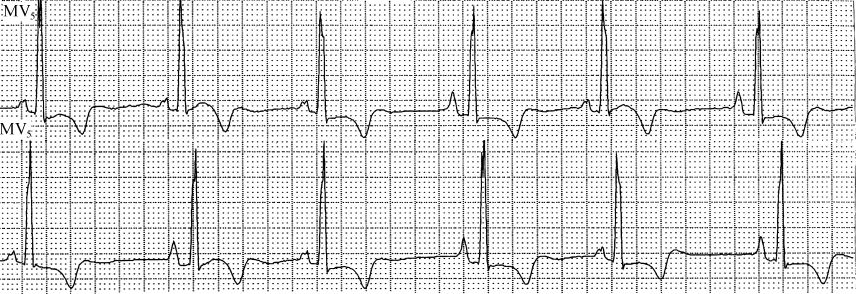
\includegraphics[width=5.78125in,height=1.97917in]{./images/Image00014.jpg}
 \captionsetup{justification=centering}
 \caption{MV\textsubscript{5}}
 \label{fig1-9}
  \end{figure} 
导联连续记录,显示4相性右心房内传导阻滞引起一过性肺型P波、ST-T改变(与图\ref{fig1-8}系同一患者)

(3)右心房内文氏现象:当P-P间期规则时,出现P波振幅由正常→较高尖→高尖→正常,周而复始有规律地改变。

(4)左心房内文氏现象:当P-P间期规则时,出现P波时间由正常→稍增宽→明显增宽→正常,周而复始有规律地改变。

\protect\hypertarget{text00007.htmlux5cux23subid10}{}{}

\subsection{右位心型P波}

心电图上具有特征性改变的是镜像右位心,有以下5个特征:

(1)Ⅰ导联上P-QRS-T波群均倒置,呈正常者的倒像。

(2)Ⅱ与Ⅲ导联、aVR与aVL导联图形互换,aVF导联图形不变。

(3)V\textsubscript{1} ~V\textsubscript{6}
导联R波振幅逐渐降低而S波则相对变深(图\ref{fig1-10}A)。

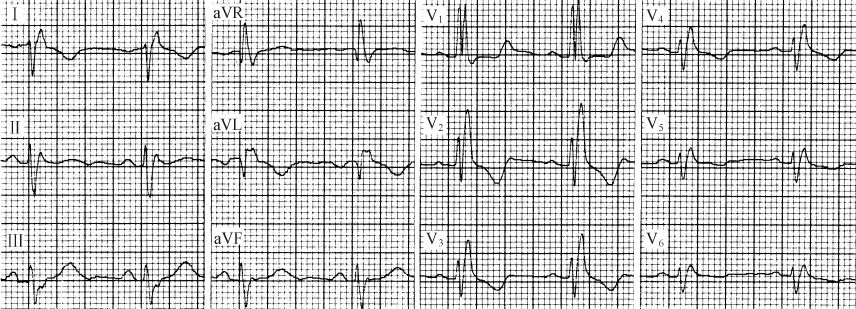
\includegraphics[width=5.78125in,height=2.08333in]{./images/Image00015.jpg}

图\ref{fig1-10}A 右位心型P波、完全性右束支传导阻滞(正常连接的十二导联)

(4)加做V\textsubscript{3} R、V\textsubscript{4} R、V\textsubscript{5}
R、V\textsubscript{6}
R导联,其R波、T波振幅逐渐增高或者以V\textsubscript{4}
R、V\textsubscript{5} R导联最高。

(5)左、右手导联线反接,胸前导联以V\textsubscript{2}
、V\textsubscript{1} 、V\textsubscript{3} R、V\textsubscript{4}
R、V\textsubscript{5} R、V\textsubscript{6}
R导联方式检查,将会显露心电图的真面目(图\ref{fig1-10}B)。

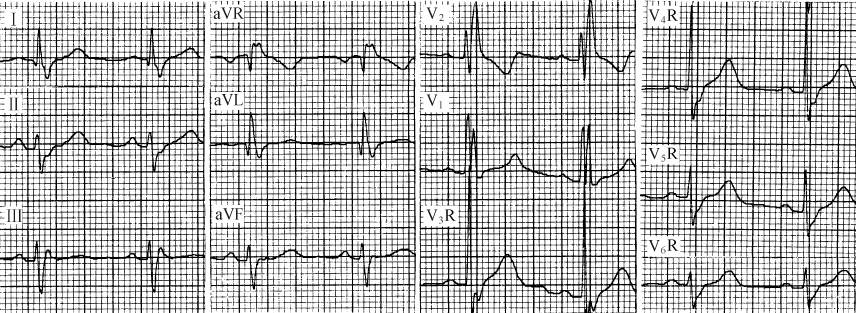
\includegraphics[width=5.78125in,height=2.11458in]{./images/Image00016.jpg}

图\ref{fig1-10}B 左、右手导联线反接及加做右胸前导联记录,显示完全性右束支传导阻滞、电轴左偏(-35°)

\protect\hypertarget{text00007.htmlux5cux23subid11}{}{}

\subsection{房间隔阻滞型P波}

房间隔阻滞型P波是指Ⅱ、Ⅲ、aVF导联P波呈正、负双相伴时间≥0.12s。见于不完全性左心房内传导阻滞伴左心房逆行传导,是一种特殊类型的心房内传导阻滞。表现为窦性冲动在左心房内除极不仅延缓,还从左心房下部向上部除极,形成终末负相P波,系上房间束(Bachmann束)传导完全阻滞所致(图\ref{fig1-11})。

\begin{figure}[!htbp]
 \centering
 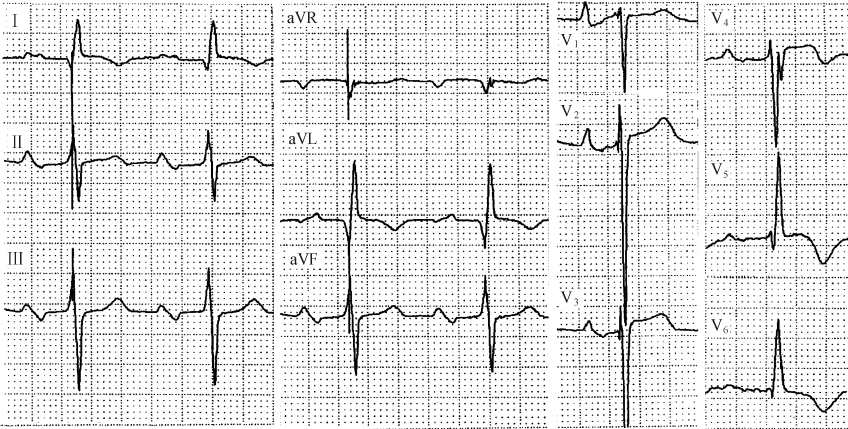
\includegraphics[width=5.72917in,height=2.89583in]{./images/Image00017.jpg}
 \captionsetup{justification=centering}
 \caption{扩张型心肌病患者出现正负双相型P波(上房间束传导阻滞所致)、右心房肥大、一度房室传导阻滞,提示房室结内双径路传导(P-R间期0.24、0.31s)、左前分支阻滞、伪室性融合波(心室起搏脉冲落在QRS波群中)、前壁r波振幅逆递增(r\textsubscript{V\textsubscript{2}}}
 \label{fig1-11}
  \end{figure} 
>r\textsubscript{V\textsubscript{3}}
>r\textsubscript{V\textsubscript{4}}
)、高侧壁异常Q波、高侧壁及前侧壁ST-T改变

1.心电图特征

(1)Ⅱ、Ⅲ、aVF导联P波呈正、负双相。

(2)P波时间≥0.12s。

(3)P波前半部分与后半部分的P环电轴夹角常>90°。

(4)心内电生理检查时,心房除极顺序为高位右心房→低位右心房→低位左心房→高位左心房。

2.鉴别诊断

需与窦性P波电轴左偏相鉴别。两者虽然均表现为Ⅱ、Ⅲ、aVF导联P波呈正、负双相,但后者P波时间正常,活动后P波转为直立,可资鉴别。

3.临床意义

(1)出现房间隔阻滞型P波是左心房扩大或肥大非常特异的征象,同时意味着上房间束传导完全阻滞。

(2)具有较高的快速性房性心律失常发生率,尤其是心房扑动。

\protect\hypertarget{text00007.htmlux5cux23subid12}{}{}

\subsection{游走性P波}

(1)窦房结内游走节律:起搏点在窦房结头、体、尾部游走不定引起P波形态、频率改变者。其心电图特征为:①P波极性一致,振幅由高→低或由低→高周期性改变,但不出现逆行P\textsuperscript{-}
波,时间多正常;②P-P间期互差>0.16s,P波振幅较高时,其P-P间期较短,P波振幅逐渐减低时,其P-P间期又逐渐延长;③P-R间期多固定(图\ref{fig1-12})。

\begin{figure}[!htbp]
 \centering
 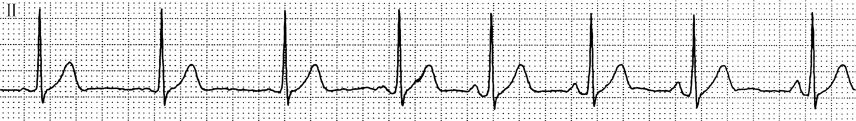
\includegraphics[width=5.78125in,height=0.8125in]{./images/Image00018.jpg}
 \captionsetup{justification=centering}
 \caption{窦房结内游走节律}
 \label{fig1-12}
  \end{figure} 

(2)窦房结至心房内游走节律:起搏点在窦房结头、体、尾部直至心房下部游走不定引起P波形态、极性和频率改变者。其心电图特征为:①P波极性有直立和倒置两种,振幅由高→低→浅倒→倒置或由倒置→浅倒→低→高周期性改变;②P-P间期不规则,P波振幅较高时,其P-P间期较短,P波振幅逐渐减低时,其P-P间期又逐渐延长;③P-R间期大多固定(图\ref{fig1-13})。

\begin{figure}[!htbp]
 \centering
 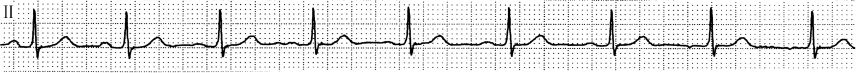
\includegraphics[width=5.78125in,height=0.48958in]{./images/Image00019.jpg}
 \captionsetup{justification=centering}
 \caption{窦房结至心房内游走节律(但不能排除非阵发性房性心动过速伴不同程度的房性融合波)}
 \label{fig1-13}
  \end{figure} 

\protect\hypertarget{text00007.htmlux5cux23subid13}{}{}

\subsection{P波低电压}

常规十二导联P波振幅均<0.1mV,称为P波低电压或振幅降低。

1.心电图特征

(1)所有导联P波振幅均<0.1mV。

(2)QRS波群低电压(肢体导联QRS波幅<0.5mV或胸前导联QRS波幅<1.0mV)。

(3)T波低平或倒置,Q-T间期延长。

(4)可出现过缓性心律失常及各种传导阻滞。

2.临床意义

(1)冲动起源于窦房结尾部。

(2)广泛而严重的心房肌纤维化。

(3)甲状腺功能减退。

(4)过度肥胖、大量心包积液或左侧气胸。

(5)高钾血症,随着血钾浓度逐渐增高,P波振幅逐渐减小直至消失。

(6)心房梗死。

\protect\hypertarget{text00007.htmlux5cux23subid14}{}{}

\subsection{P波电交替}

1.心电图特征

(1)P-P间期、P-R间期均必须固定,以确保是同一起搏点的激动,多见于窦性节律。

(2)交替出现两种形态的窦性P波,其振幅互差≥0.1mV,时间可有轻度互差。

(3)两种形态P波的极性一致,其额面P环电轴指向左下。

(4)这两种P波形态的改变与呼吸、伪差等心外因素无关(图\ref{fig1-14})。

(5)可伴有QRS波幅、ST段、T波、U波电交替现象。

\begin{figure}[!htbp]
 \centering
 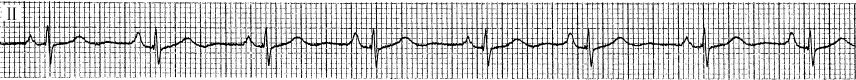
\includegraphics[width=5.78125in,height=0.53125in]{./images/Image00020.jpg}
 \captionsetup{justification=centering}
 \caption{P波电交替现象}
 \label{fig1-14}
  \end{figure} 

2.发生机制

(1)心房内特殊传导组织或某部分心房肌传导障碍,导致交替性心房内传导阻滞。

(2)心房肌缺血致跨膜动作电位复极2相、3相发生交替性改变或心房肌不应期长、短交替性改变,导致交替性心房肌除极异常。

(3)窦房结头部与尾部交替性发放冲动,此时其P-P间期略有互差。

(4)窦房交接区双径路(双出口)交替传导,导致心房除极顺序发生改变。

(5)左、右心房起搏点等频性交替性发放冲动,形成双源性房性心律,或窦房结与心房异位起搏点交替性发放冲动。严格地说,这两种情况不属于P波电交替范畴内。

3.临床意义

(1)这是一种罕见的心电现象,多见于器质性心脏病,如心房梗死、心房负荷过重、心房扩大及心房肌严重缺血等,常提示心房病变严重而广泛,是一种预后不良的征象,死亡率较高。

(2)这是心房肌严重缺血、心电不稳定的表现,易发生各种房性心律失常。

\protect\hypertarget{text00007.htmlux5cux23subid15}{}{}

\subsection{P波缺失}

(一)一过性窦性P波缺失

1.窦性停搏

(1)心电图特征:①长P-P间期与短P-P间期之间无倍数关系;②长P-P间期>1.80~2.0s(白天1.80s,夜间2.0s)或长P-P间期大于短P-P间期的1.5倍(图\ref{fig1-15})。

\begin{figure}[!htbp]
 \centering
 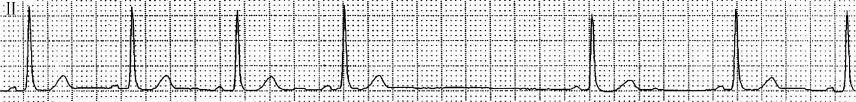
\includegraphics[width=5.78125in,height=0.6875in]{./images/Image00021.jpg}
 \captionsetup{justification=centering}
 \caption{窦性心律不齐、窦性停搏}
 \label{fig1-15}
  \end{figure} 

(2)临床意义:①心源性窦房结功能障碍:又称为原发性病窦综合征,多由器质性心脏病所致;②外源性窦房结功能障碍:又称为继发性病窦综合征,多由心脏活性药物、迷走神经张力显著增高、低温、高钾血症、重度颅脑损伤等心外因素所致,以前两者影响最为重要;③特发性窦房结功能障碍:经多种检查无法明确病因,又无心脏病基础者。

2.窦房传导阻滞

(1)二度Ⅰ型窦房传导阻滞:P-P间期逐渐缩短直至出现1个长P-P间期,长P-P间期小于任何短P-P间期的2倍,P-P间期呈“渐短突长”规律,周而复始。

(2)二度Ⅱ型窦房传导阻滞:长P-P间期为短P-P间期的2~3倍(图\ref{fig1-16})。

(3)高度~几乎完全性窦房传导阻滞:长P-P间期≥4倍的短P-P间期。

\begin{figure}[!htbp]
 \centering
 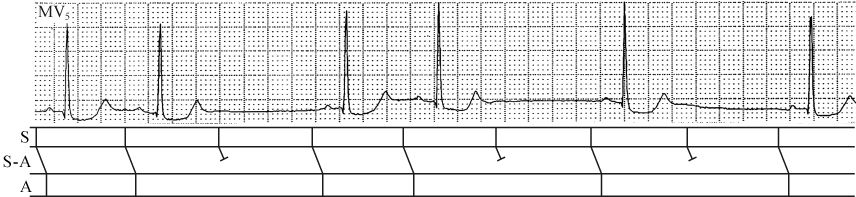
\includegraphics[width=5.78125in,height=1.32292in]{./images/Image00022.jpg}
 \captionsetup{justification=centering}
 \caption{二度Ⅱ型窦房传导阻滞、ST段呈缺血型改变}
 \label{fig1-16}
  \end{figure} 

3.窦房结节律超速抑制现象。

见于短阵性房性心动过速、阵发性心房扑动、心房颤动或阵发性室上性心动过速等快速性异位心律终止后对窦房结节律的超速抑制。异位节律的频率愈快、持续时间愈长、窦房结功能愈差者,则窦性节律恢复所需的时间愈长(图\ref{fig1-17})。

\begin{figure}[!htbp]
 \centering
 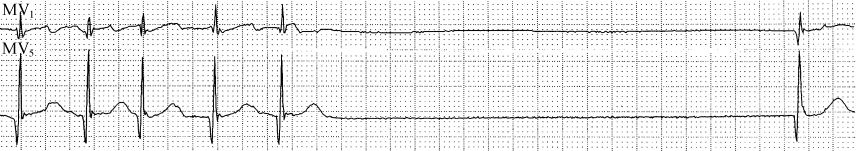
\includegraphics[width=5.78125in,height=1.02083in]{./images/Image00023.jpg}
 \captionsetup{justification=centering}
 \caption{阵发性不纯性心房扑动终止后出现短暂性全心停搏、过缓的房室交接性逸搏}
 \label{fig1-17}
  \end{figure} 

4.窦性节律被重整或干扰性窦房分离。

下级起搏点自律性增高,如加速的房性逸搏心律、加速的房室交接性逸搏心律等异位冲动逆传窦房结使其节律连续重整或与窦性冲动在窦房交接区产生连续干扰形成不完全性干扰性窦房分离。

(二)较长时间窦性P波缺失

(1)窦性停搏:基本节律可为房性、房室交接性、室性逸搏心律或人工起搏心律等。

(2)三度窦房传导阻滞。

(3)窦-室传导:见于高钾血症,血钾恢复正常后,将出现窦性P波。

(4)阵发性室上性心动过速、阵发性心房扑动及心房颤动发作期间。

(5)加速的房性逸搏心律、加速的房室交接性逸搏心律等异位冲动持续重整窦性节律,形成假性窦性停搏或与窦性冲动在窦房交接区产生连续干扰形成干扰性窦房分离(假性三度窦房传导阻滞)。

(三)永久性窦性P波缺失

1.永久性三度窦房传导阻滞

2.永久性窦性停搏

3.永久性心房颤动

4.隐匿性窦性心律

(1)概念:指常规心电图中始终未见窦性P波,但经心房内或食管内心电图能记录到窦性P波一种少见的心电现象。

(2)心电图特征:①常规心电图始终未见心房电活动波,如P波、P\textsuperscript{-}
波、F波或f波;②QRS波形正常或显示心室肥大、束支阻滞等图形,R-R间期符合窦性心律标准;③做心房内或食管内心电图时,可见QRS波群之前有A波或窦性P波,两者具有相关性。

5.心房静止

(1)概念:指心房肌因严重而广泛的不可逆损害,导致心房肌应激性丧失使其永久不能除极。

(2)心电图特征:①体表心电图、食管心电图、心房内心电图均未见P波或A波;②对心房肌进行电刺激时仍未见心房电活动;③X线胸透、超声心动图检查亦未见心房肌收缩活动;④QRS波形正常,基本节律起源于房室交接区。

(3)临床意义:①多见于器质性心脏病;②偶见于先天性心房肌应激功能异常。

\protect\hypertarget{text00007.htmlux5cux23subid16}{}{}

\subsection{窦性早搏}

1.心电图特征

(1)提早出现的P′波形态与同导联的窦性P波一致或略异。这取决于该早搏起搏点的位置、传出途径与窦性激动是否一致。

(2)呈等周期代偿,即P′-P间期等于窦性P-P间期。

(3)P′波下传的P′-R间期正常或呈干扰性P′-R间期延长,QRS波形正常或伴心室内差异性传导。

(4)偶联间期固定者,为折返型早搏;若偶联间期不等,两异位搏动之间相等或有一最大公约数,则为并行心律型早搏;否则为异位自律性增高型早搏(图\ref{fig1-18})。

\begin{figure}[!htbp]
 \centering
 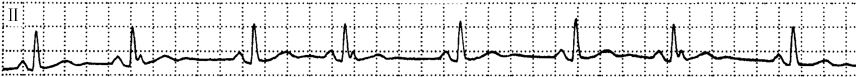
\includegraphics[width=5.78125in,height=0.51042in]{./images/Image00024.jpg}
 \captionsetup{justification=centering}
 \caption{舒张晚期窦性早搏,呈二、三联律}
 \label{fig1-18}
  \end{figure} 

2.临床意义

(1)窦性早搏的出现,改变了早搏都是由异位起搏点发放冲动的观念,早搏也可发生在正常起搏点内。

(2)可以是功能性的,由心外因素所致;也可以是器质性的,由器质性心脏病所致。

\protect\hypertarget{text00007.htmlux5cux23subid17}{}{}

\subsection{窦性逸搏}

1.心电图特征

(1)在两阵快速或较快速异位性心动过速终止后间歇期内,略为延迟出现1~2次窦性搏动,其P波形态与正常窦性P波一致。

(2)若逸搏周期0.60~1.0s,频率60~100次/min,则称为窦性逸搏;若逸搏周期>1.0s,频率<60次/min,则称为过缓的窦性逸搏。

(3)若连续出现≥3次窦性逸搏,则称为窦性逸搏心律,亦称为正常的窦性心律。

2.临床意义

(1)窦性逸搏的出现,仍标志着窦房结有正常的起搏功能,出现窦性逸搏是由于下级起搏点发放快速或较快速激动后又突然终止所致。若异位节律点得到控制后,将自然恢复正常的窦性心律。

(2)过缓的窦性逸搏常见于窦房结自律性降低或病窦综合征患者,转复为窦性心律后,可出现窦性停搏。

\protect\hypertarget{text00007.htmlux5cux23subid18}{}{}

\subsection{窦性回波及窦房交接性早搏}

严格地说,窦性回波及窦房交接性早搏不属于窦性P波的范畴,但因其P波形态与窦性P波一致或相似,故放在此处讨论。

1.窦性回波

(1)发生机制:窦房结及其周围组织的电生理功能和房室结有一定的相似性,细胞间的不应期和传导性均存在明显差异,窦房结及窦房交接区可分离为两条传导功能不同的径路。适时的房性早搏由一条径路逆传侵入窦房结,再经另一条径路传出,再次激动心房,形成窦性回波。在房性早搏后,产生P′-P\textsubscript{3}
-P\textsubscript{4} 序列,其中P\textsubscript{3}
为窦性回波,P\textsubscript{4}
为房性早搏重整窦性节律后窦性所发放的第1个激动,上述P′-P\textsubscript{3}
-P\textsubscript{4} 序列中的P\textsubscript{3} -P\textsubscript{4}
间期小于窦性P\textsubscript{1} -P\textsubscript{2} 间期(图\ref{fig1-19})。

(2)心电图特征:①适时的房性早搏(P′波)或有逆传心房的房室交接性早搏、室性早搏后,紧跟1个与窦性P波(P\textsubscript{1}
、P\textsubscript{2} 、P\textsubscript{4}
)形态相同的P波(P\textsubscript{3}
);②窦房折返周期P′-P\textsubscript{3} 间期<P\textsubscript{1}
-P\textsubscript{2}
间期;③房性早搏的偶联间期多在0.25~0.46s之间,方能引起窦性回波P\textsubscript{3}
;④P\textsubscript{2} -P\textsubscript{3} 间期不等于P\textsubscript{1}
-P\textsubscript{2}
间期,可排除P′波为间位型房性早搏;⑤P\textsubscript{3}
-P\textsubscript{4} 间期<P\textsubscript{1} -P\textsubscript{2}
间期,可排除P′、P\textsubscript{3} 波为成对房性早搏(图\ref{fig1-19})。

\begin{figure}[!htbp]
 \centering
 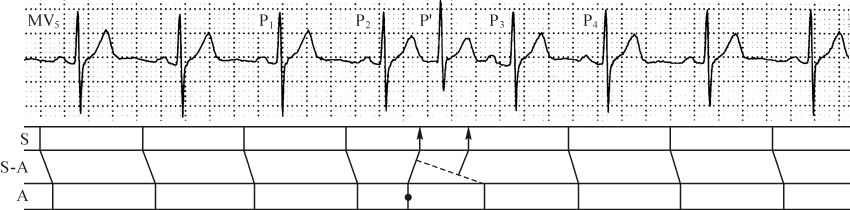
\includegraphics[width=5.73958in,height=1.41667in]{./images/Image00025.jpg}
 \captionsetup{justification=centering}
 \caption{房性早搏诱发窦性回波}
 \label{fig1-19}
  \end{figure} 

2.窦房交接性早搏

(1)提早出现的P′波形态与窦性P波一致或略异。这取决于该早搏激动下传途径与窦性激动是否一致、心房除极顺序有无改变。

(2)可呈次等周期、等周期代偿或不完全性代偿间歇。这取决于窦房交接性早搏逆传重整窦性节律所需时间与前传激动心房所需时间差值的多少和窦房结节律的稳定性。在窦性节律规则时,当逆传重整窦性节律先于前传激动心房,且两者时间差刚好为窦房传导时间,则呈等周期代偿(图\ref{fig1-20}A),与窦性早搏难以鉴别;当逆传重整窦性节律明显先于前传激动心房,则呈次等周期代偿(图\ref{fig1-20}B);反之,当前传激动心房明显先于逆传重整窦性节律,则呈不完全性代偿间歇(图\ref{fig1-20}C),与房性早搏难以鉴别。故只有呈次等周期代偿时方能诊断。

\begin{figure}[!htbp]
 \centering
 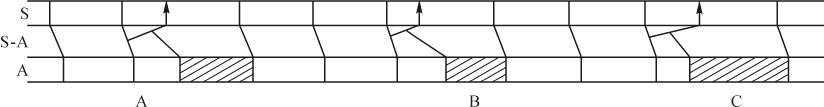
\includegraphics[width=5.5625in,height=0.71875in]{./images/Image00026.jpg}
 \captionsetup{justification=centering}
 \caption{窦房交接性早搏出现3种代偿间歇的梯形图解模式(图A:等周期代偿;图B:次等周期代偿;图C:不完全性代偿间歇)}
 \label{fig1-20}
  \end{figure} 

(3)P′波下传的P′-R间期正常或伴干扰性P′-R间期延长,QRS波形正常或伴心室内差异性传导。

(4)偶联间期多固定(图\ref{fig1-21})。

\begin{figure}[!htbp]
 \centering
 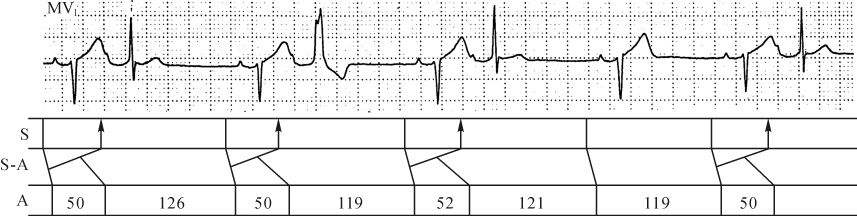
\includegraphics[width=5.79167in,height=1.45833in]{./images/Image00027.jpg}
 \captionsetup{justification=centering}
 \caption{窦房交接区折返性早搏伴心室内差异性传导(呈左中隔支阻滞型及右束支阻滞型)}
 \label{fig1-21}
  \end{figure} 

\protect\hypertarget{text00007.htmlux5cux23subid19}{}{}

\section{异位P波}

\protect\hypertarget{text00007.htmlux5cux23subid20}{}{}

\subsection{逆行P\textsuperscript{-} 波}

1.基本概念

起源于心房下部、房室交接区或心室异位激动逆传心房时所产生的P波极性与窦性P波刚好相反,称为逆行P\textsuperscript{-}
波,常用P\textsuperscript{-} 表示。

2.心电图特征

(1)P\textsuperscript{-} 波在Ⅱ、Ⅲ、aVF导联倒置,aVR导联直立。

(2)根据P\textsuperscript{-}
-R间期的长短来判断异位起搏点的位置:若P\textsuperscript{-}
-R间期≥0.12s,则起源于心房下部(图\ref{fig1-22});若P\textsuperscript{-}
-R间期<0.12s,则起源于房室交接区(图\ref{fig1-23})。

\begin{figure}[!htbp]
 \centering
 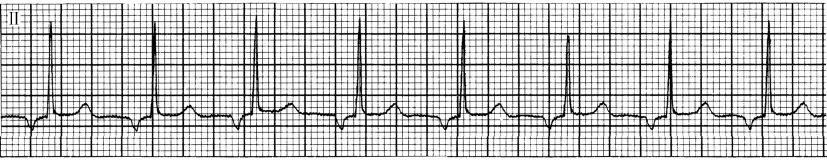
\includegraphics[width=5.58333in,height=1.07292in]{./images/Image00028.jpg}
 \captionsetup{justification=centering}
 \caption{加速的房性逸搏心律(起源于心房下部,其P\textsuperscript{-}}
 \label{fig1-22}
  \end{figure} 
-R间期0.14s,频率92次/min)

\begin{figure}[!htbp]
 \centering
 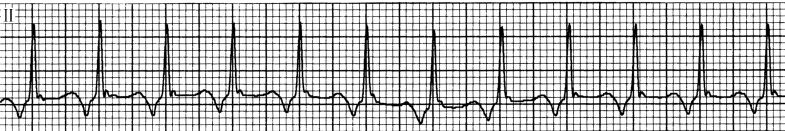
\includegraphics[width=5.30208in,height=0.88542in]{./images/Image00029.jpg}
 \captionsetup{justification=centering}
 \caption{男性患者发生心动过速半年余,提示持续性房室交接性心动过速(P\textsuperscript{-}}
 \label{fig1-23}
  \end{figure} 
-R间期0.10s,频率150次/min)

(3)若逆行P\textsuperscript{-}
波位于QRS波群之后,则根据R-P\textsuperscript{-}
间期的长短、QRS波形的特征来判断异位起搏点的位置:若R-P\textsuperscript{-}
间期≤0.16s,QRS波形正常,则起源于房室交接区;若R-P\textsuperscript{-}
间期>0.16s,QRS波群宽大畸形,则起源于心室。

\protect\hypertarget{text00007.htmlux5cux23subid21}{}{}

\subsection{正相逆行P\textsuperscript{-} 波}

1.基本概念

起源于房室交接区或心室异位激动逆传心房时所产生的逆行P\textsuperscript{-}
波,在Ⅱ、Ⅲ、aVF导联呈直立P波,称为正相逆行P\textsuperscript{-} 波。

2.心电图特征

(1)房室交接性心律伴正相逆行心房夺获。

(2)房室交接性或室性心律不齐时,在其QRS波群后面始终跟随与R波有固定关系的正相P波。

(3)与P-R间期延长到某临界值相关联的提早出现的正相P波或(和)反复性心动过速(图\ref{fig1-24})
。

(4)预激综合征时,出现正相P波的反复性心动过速。

\begin{figure}[!htbp]
 \centering
 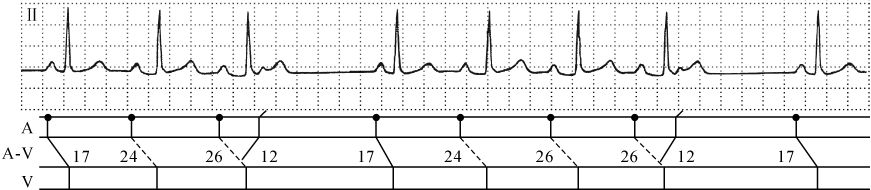
\includegraphics[width=5.88542in,height=1.28125in]{./images/Image00030.jpg}
 \captionsetup{justification=centering}
 \caption{房室结双径路传导伴慢径路文氏现象及正相逆行P\textsuperscript{-}}
 \label{fig1-24}
  \end{figure} 
波(引自郑莹)

3.发生机制

心房内的特殊传导纤维,如结间束、James束(大部分由后结间束组成,少部分由前、中结间束组成)及Kent束的存在为正相逆行P\textsuperscript{-}
波的解释提供了解剖学基础。当起源于房室交接区或心室异位激动经房室正道逆传受阻时,可从James束或从出口处位于心房上部的Kent束逆传,使心房除极顺序与窦性激动相似而出现直立P波,或房室交接区激动优先通过前结间束快速逆行到房间束和窦房交接区先激动心房上部,使心房除极顺序与窦性激动相似,也可出现直立P波。

\protect\hypertarget{text00007.htmlux5cux23subid22}{}{}

\subsection{房性早搏}

1.心电图特征

(1)提早出现的P′波形态与窦性P波不一致,有时P′波重叠在T波上使T波变形。不论其后是否跟随QRS-T波群,均可作出房性早搏的诊断。

(2)多呈不完全性代偿间歇,舒张晚期的房性早搏可出现完全性代偿间歇。

(3)发生在收缩中、晚期及少数舒张早期的房性早搏,将出现各种房室干扰现象,如呈阻滞型、房室结内隐匿性传导、干扰性P′-R间期延长及心室内差异性传导,其中前两者称为房性早搏未下传(图\ref{fig1-25})。

(4)若P′波形态不一致而偶联间期相等,则为多形性房性早搏;若P′波形态及偶联间期均不相同,则为多源性房性早搏。

\begin{figure}[!htbp]
 \centering
 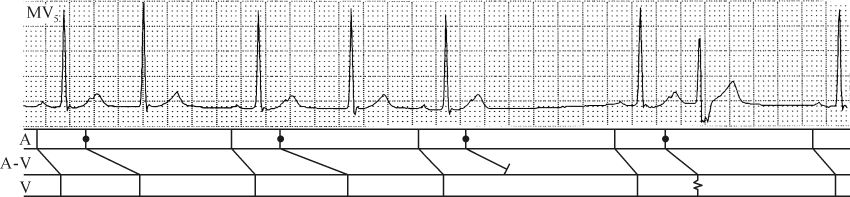
\includegraphics[width=5.73958in,height=1.32292in]{./images/Image00031.jpg}
 \captionsetup{justification=centering}
 \caption{房性早搏二联律伴房室干扰现象(P′波未下传、干扰性P′-R间期延长及心室内差异性传导),其中最后1个房性早搏下传的P′-R间期明显缩短,可能与房室结2相超常期传导有关}
 \label{fig1-25}
  \end{figure} 

2.临床意义

(1)功能性房性早搏:由心外因素所致。

(2)器质性房性早搏:由器质性心脏病所致。

(3)药物性房性早搏:由各种药物过量或毒副作用所致。

\protect\hypertarget{text00007.htmlux5cux23subid23}{}{}

\subsection{房性逸搏}

1.心电图特征

(1)在两阵窦性心律或两阵异位心律之间,延迟出现1~2次P′波或P′-QRS-T波群,P′波形态与窦性P波不同。若P′波形态一致,则为单源性房性逸搏;若P′波呈两种形态,则为双源性房性逸搏(图\ref{fig1-26});若P′波呈3种或3种以上形态,则称为多源性房性逸搏。

\begin{figure}[!htbp]
 \centering
 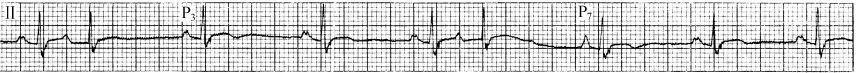
\includegraphics[width=5.78125in,height=0.48958in]{./images/Image00032.jpg}
 \captionsetup{justification=centering}
 \caption{折返型房性早搏后出现双源性房性逸搏(P\textsubscript{3}}
 \label{fig1-26}
  \end{figure} 
、P\textsubscript{7} ),但不能排除窦性P波伴非时相性心房内差异性传导

(2)若逸搏周期1.0~1.20s,频率50~60次/min,则称为房性逸搏;若逸搏周期>1.20s,频率<50次/min,则称为过缓的房性逸搏;若逸搏周期0.60~1.0s,频率61~100次/min,则称为加速的房性逸搏。

(3)P′-R间期、QRS波形与窦性一致。有时房性逸搏P′波刚出现时,又发生了房室交接性逸搏或室性逸搏,则P′-R间期<0.12s,P′波被干扰而未能下传。

(4)有时可见延迟出现的P′波与窦性P波相融合,而成为房性融合波。

2.房性逸搏的定位诊断(见第十一章第四节房性早搏的定位诊断)

3.临床意义

房性逸搏及其逸搏心律的出现,表明心脏有潜在的起搏能力,它本身并无重要临床意义,主要取决于原发性心律失常。而加速的房性逸搏及其逸搏心律的出现,若不伴有窦性节律竞争,则说明窦房结自律性降低,部分见于器质性心脏病,如冠心病、病窦综合征等,部分则无器质性心脏病。若伴有窦房结-心房节律竞争,则见于心肌炎、急性心肌梗死、洋地黄中毒、心脏手术等。

\protect\hypertarget{text00007.htmlux5cux23subid24}{}{}

\section{房性融合波}

1.基本概念

发自心脏两个节律点的冲动从不同方向同时进入心房,且各自激动了心房的一部分,此时所形成的P波称为房性融合波。房性融合波是心房内绝对干扰所致。

2.心电图特征

(1)房性融合波的形态介于其他两种P波之间,视融合程度不同,其形态可以多变。

(2)房性融合波出现的时间必须是两个节律点冲动同时或几乎同时出现的时间。

3.房性融合波的类型

(1)窦性P波与房性P′波之间的融合:该P′波可以是舒张晚期房性早搏、房性逸搏或人工心房起搏搏动等。

(2)窦性P波与逆行P\textsuperscript{-}
波之间的融合:该逆行P\textsuperscript{-}
波可以是起源于心房下部、房室交接区或心室异位搏动逆传心房时产生(图\ref{fig1-27})。

\begin{figure}[!htbp]
 \centering
 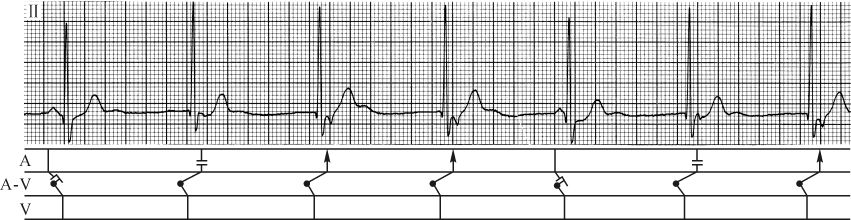
\includegraphics[width=5.75in,height=1.47917in]{./images/Image00033.jpg}
 \captionsetup{justification=centering}
 \caption{窦性心动过缓、房室交接性逸搏心律及房性融合波}
 \label{fig1-27}
  \end{figure} 

(3)心房内两个异位P′波之间的融合:心房内有两个异位起搏点几乎同时发放冲动,各自激动了心房的一部分。见于双重性房性并行心律、多源性房性早搏、多源性房性心动过速等。

(4)房性异位P′波与逆行P\textsuperscript{-} 波之间的融合。

4.鉴别诊断

主要与心房分离时所出现的重叠波相鉴别,即心房分离时所产生的低小P′波重叠在主导节律所产生的P波不同部位上。两者是重叠而不是融合(详见第十九章第三节局限性完全性心房内传导阻滞)。

\protect\hypertarget{text00007.htmlux5cux23subid25}{}{}

\section{心房内差异性传导}

\protect\hypertarget{text00007.htmlux5cux23subid26}{}{}

\subsection{时相性心房内差异性传导}

1.心电图特征

(1)提早出现变形的P、P′或P\textsuperscript{-}
波,不能用其他原因解释者。

(2)窦性早搏伴心房内差异性传导:窦性早搏的P波形态与其他窦性P波形态不同。

(3)房性早搏伴心房内差异性传导:房性早搏的P′波形态明显畸形,可呈肺型P波或二尖瓣型P波特点(图\ref{fig1-28})。

\begin{figure}[!htbp]
 \centering
 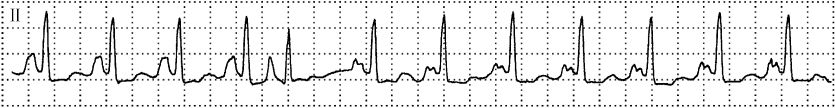
\includegraphics[width=5.64583in,height=0.72917in]{./images/Image00034.jpg}
 \captionsetup{justification=centering}
 \caption{房性早搏伴心房内差异性传导、间歇性不完全性左右心房内传导阻滞、ST段改变}
 \label{fig1-28}
  \end{figure} 

(4)房室交接性早搏或室性早搏逆传心房时伴心房内差异性传导:逆行P\textsuperscript{-}
波形态明显畸形,通常是P\textsuperscript{-}
波倒置加深或增宽呈反向“二尖瓣型P波” 。

2.发生机制

时相性心房内差异性传导(简称心房内差异性传导)系心房内相对干扰所致,主要与冲动过早出现遇及心房内传导组织(如结间束、Bachmann束)和心房肌相对不应期有关。

3.临床意义

因心房内传导组织、心房肌不应期均较短,一般情况下极少发生心房内差异性传导。一旦出现,则意味着心房有病变,多见于器质性心脏病患者。

\protect\hypertarget{text00007.htmlux5cux23subid27}{}{}

\subsection{非时相性心房内差异性传导}

1.心电图表现

(1)房性早搏、短阵性房性心动过速或能逆传心房的房室交接性早搏、室性早搏代偿间歇之后,出现1个或连续数个窦性P波形态发生改变。

(2)变形的P波又是窦性P波应出现的位置,且多次重复出现(图\ref{fig1-29})。

\begin{figure}[!htbp]
 \centering
 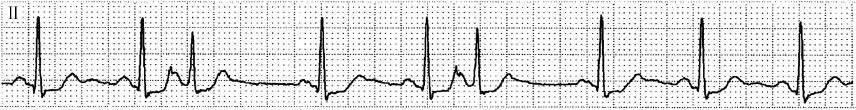
\includegraphics[width=5.78125in,height=0.73958in]{./images/Image00035.jpg}
 \captionsetup{justification=centering}
 \caption{折返型房性早搏后出现非时相性心房内差异性传导、轻度ST段改变}
 \label{fig1-29}
  \end{figure} 

2.发生机制

(1)早搏在心房传导组织内发生隐匿性传导:由于结间束、房间束的不应期不一致,早搏在逆传窦房结时,可在窦房交接区内产生隐匿性折返,并隐匿性地激动了结间束、房间束,使其产生新的不应期,影响下一个窦性激动的正常除极,导致P波形态改变。

(2)心房内4相性传导阻滞:早搏产生较长的代偿间歇,结间束或房间束发生4相性传导阻滞。

3.鉴别诊断

应注意与窦房结内游走节律、窦房结至心房内游走节律、房性逸搏及房性融合波相鉴别。

4.临床意义

见于器质性心脏病患者。常出现在心力衰竭患者,具有病理意义。

\protect\hypertarget{text00008.html}{}{}

\protect\hypertarget{text00008.htmlux5cux23chapter8}{}{}

\chapter{PR段偏移和P-R间期异常及P-J间期}

\protect\hypertarget{text00008.htmlux5cux23subid28}{}{}

\section{PR段偏移}

心房除极结束后至心室开始除极前,有一段无电位差的等电位线,称为PR段,通常以TP段的延长线作为基线。PR段常受Ta波的影响,可呈下斜型压低(≤0.08~0.1mV)或抬高(≤0.05mV)。

1.心电图特征

在P波明显的导联出现PR段压低(>0.08~0.1mV)或抬高(>0.05mV),特别是呈水平型压低时,则属异常改变,对心房梗死、急性心包炎、心房损伤等有较大的诊断价值(图\ref{fig2-1})。

\begin{figure}[!htbp]
 \centering
 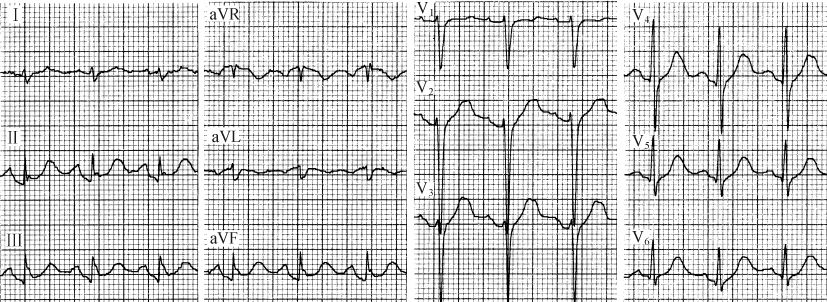
\includegraphics[width=5.58333in,height=2.04167in]{./images/Image00036.jpg}
 \captionsetup{justification=centering}
 \caption{急性心包炎患者出现窦性心动过速、肢体导联QRS波群低电压倾向、PR段压低}
 \label{fig2-1}
  \end{figure} 

2.临床意义

(1)心房梗死:单纯性心房梗死罕见,多与心室梗死并存,常伴发快速性房性心律失常。

(2)急性心包炎:PR段偏移可能是急性心包炎最早出现的心电图异常,甚至是唯一可见的心电图改变,具有较高的特异性。

(3)心房肌劳损、心房外伤。

(4)心房肥大或扩大。

\protect\hypertarget{text00008.htmlux5cux23subid29}{}{}

\section{P-R间期异常改变}

\protect\hypertarget{text00008.htmlux5cux23subid30}{}{}

\subsection{P-R间期测量方法}

12导联同步记录时,以最早的P波起点至最早的QRS波群起点的间距作为P-R间期。若是3导联同步记录或单导联记录时,则选取2~3个P波最清晰、最宽大且有明显Q波(或q波)的“半正交”导联,如Ⅱ、Ⅲ、V\textsubscript{1}
(V\textsubscript{5} )或Ⅰ(aVL)、aVF、V\textsubscript{2}
(V\textsubscript{5}
)(P波电轴左偏时),按P-R间期最长者计算。其正常值为0.12~0.20s。

\protect\hypertarget{text00008.htmlux5cux23subid31}{}{}

\subsection{P-R间期缩短}

1.基本概念

P-R间期缩短仅指窦性P波、直立的房性异位P′波的P(P′)-R间期≤以下最低值:3岁以下0.08s,4~16岁0.10s,16岁以上0.11s。多表现为PR段缩短。

2.常见原因

(1)L-G-L综合征。

(2)W-P-W综合征。

(3)测量误差和年龄因素:少年儿童的房室结发育尚未完全,具有较快的传导功能。

(4)交感神经张力增高和心率增快:如发烧、运动、甲状腺功能亢进等因素可导致房室结的不应期缩短,传导速度加快。

(5)药物影响:如阿托品、肾上腺素、异丙基肾上腺素、洋地黄、糖皮质激素等均可加速房室传导。

(6)房室结加速传导现象:解剖学上较小的房室结、房室结发育不良、房室结内残存具有较快传导功能的特殊组织。

(7)正常的个体差异:成人短P-R间期并不一定反映传导异常。有报告显示,正常人群中P-R≤0.11s和≥0.21s者各占2\%,≤0.09s和≥0.24s者各占0.6\%、0.8\%。

(8)部分孕妇常出现短P-R间期(图\ref{fig2-2})。

\begin{figure}[!htbp]
 \centering
 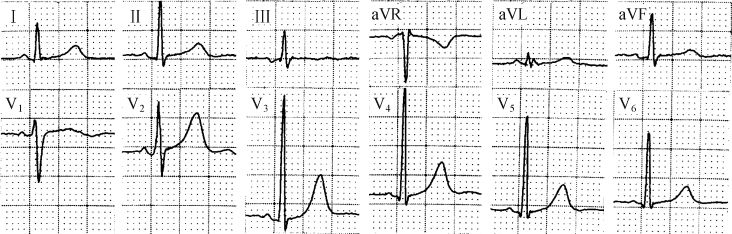
\includegraphics[width=4.94792in,height=1.57292in]{./images/Image00037.jpg}
 \captionsetup{justification=centering}
 \caption{孕妇(妊娠34周)出现短P-R间期}
 \label{fig2-2}
  \end{figure} 

(9)等频性干扰性房室分离时出现钩拢现象,常引起假性的短P-R间期(图\ref{fig2-3})。

\begin{figure}[!htbp]
 \centering
 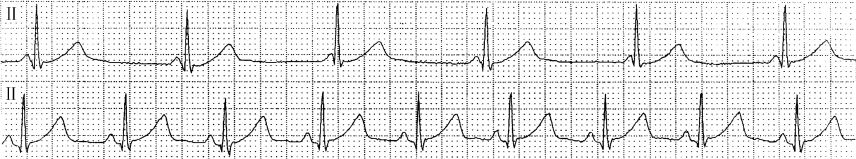
\includegraphics[width=5.78125in,height=1.07292in]{./images/Image00038.jpg}
 \captionsetup{justification=centering}
 \caption{上行显示窦性心动过缓、房室交接性逸搏心律、等频性干扰性房室分离引起房室钩拢现象及伪短P-R间期(下行系活动后记录)}
 \label{fig2-3}
  \end{figure} 

(10)部分室性融合波:室性异位搏动与窦性搏动在心室内融合出现1个或数个较短的P-R间期。

3.L-G-L综合征

窦性激动通过James束下传心室,又称为房-结旁道或房-束(希氏束)旁道或短P-R间期综合征,无房室交接区生理性0.05~0.10s延搁。其特征:①P-R间期≤0.11s;②无“δ”波,QRS波形、时间均正常或呈束支阻滞型;③有反复发作心动过速史。若仅有P-R间期缩短、QRS波形正常,临床上无反复发作心动过速史,则不宜诊断为L-G-L综合征,而应诊断为短P-R间期(图\ref{fig2-4})。

\begin{figure}[!htbp]
 \centering
 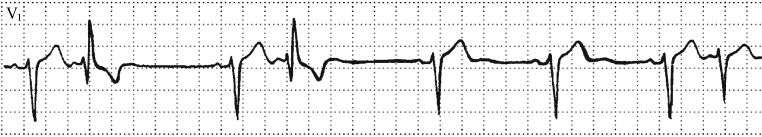
\includegraphics[width=5.14583in,height=0.91667in]{./images/Image00039.jpg}
 \captionsetup{justification=centering}
 \caption{特发性心房颤动患者出现房性早搏经James束下传(窦性P-R间期0.14s、房早P′-R间期0.08~0.10s)伴心室内差异性传导、James束内4相阻滞}
 \label{fig2-4}
  \end{figure} 

4.W-P-W综合征

窦性或房性激动通过Kent束下传心室,称为W-P-W综合征,又称为房-室旁道或典型预激综合征,属同源性室性融合波。其心电图特征:①P-R间期多为0.08~0.11s;②有“δ”波;③QRS波群时间≥0.11s;④P-J间期正常(≤0.27s);⑤有继发性ST-T改变。根据胸前导联QRS主波方向,W-P-W综合征分为A、B、C三型(图\ref{fig2-5}、图\ref{fig2-6})。

\begin{figure}[!htbp]
 \centering
 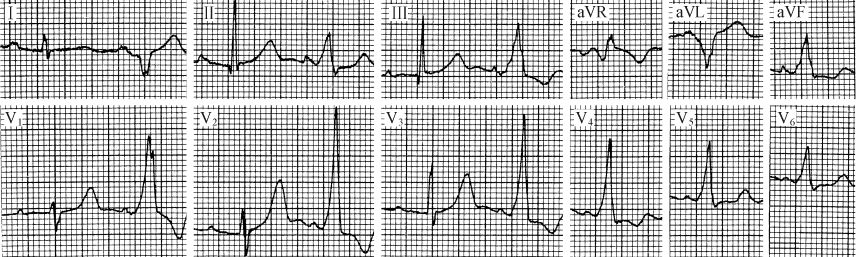
\includegraphics[width=5.78125in,height=1.72917in]{./images/Image00040.jpg}
 \captionsetup{justification=centering}
 \caption{交替性A型预激综合征、一度房室传导阻滞(P-R间期0.24s)}
 \label{fig2-5}
  \end{figure} 

\begin{figure}[!htbp]
 \centering
 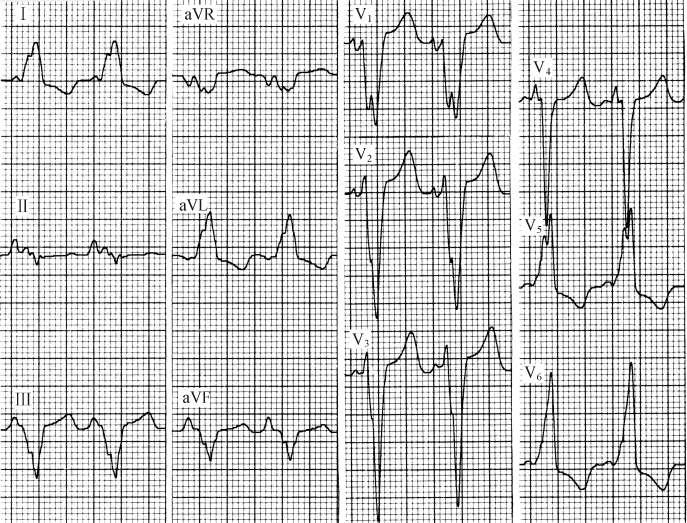
\includegraphics[width=4.64583in,height=3.53125in]{./images/Image00041.jpg}
 \captionsetup{justification=centering}
 \caption{扩张型心肌病患者出现右心房肥大(Ⅱ、aVF导联P波电压0.25~0.3mV)、B型预激综合征}
 \label{fig2-6}
  \end{figure} 

\protect\hypertarget{text00008.htmlux5cux23subid32}{}{}

\subsection{P-R间期延长}

(一)引起P-R间期延长的常见原因

正常P-R间期0.12~0.20s,当P-R间期≥0.21s时,便称为P-R间期延长,见于下列6种情况。

1.房室传导延缓

在一般情况下,同一患者在心率相近时,前后两次心电图相互比较,出现P-R间期互差≥0.04~0.05s时,便认为已发生一度房室传导阻滞。既然P-R间期正常最高值为0.20s,似应将P-R间期≥0.24s诊断为一度房室传导阻滞,0.21~0.23s诊断为房室传导延缓更为恰当。

2.一度房室传导阻滞

(1)心电图特征:①P-R间期≥0.24s(儿童≥0.21s);②同一患者在心率基本相近时,其P-R间期有动态变化且≥0.04~0.05s时,即使延长后的P-R间期在正常范围内,也应诊断为一度房室传导阻滞。实际上动态变化的P-R间期延长,其临床意义更大。

(2)阻滞类型:①一度Ⅰ型房室传导阻滞:其P-R间期逐搏延长或逐搏缩短,但未出现心室漏搏(图\ref{fig2-7});②一度Ⅱ型房室传导阻滞:其P-R间期固定地延长,即通常所说的一度房室传导阻滞;③一度Ⅲ型房室传导阻滞:延长的P-R间期长短不一,与迷走神经张力波动有关;④3相性一度房室传导阻滞:心率增快时出现P-R间期延长,而心率减慢或长间歇后P-R间期恢复正常(图\ref{fig2-8});⑤4相性一度房室传导阻滞:心率减慢或长间歇后出现P-R间期延长,而心率增快时P-R间期恢复正常(图\ref{fig2-9});⑥间歇性一度房室传导阻滞:P-R间期延长与心率快、慢无关,可能存在房室结内双径路传导。

\begin{figure}[!htbp]
 \centering
 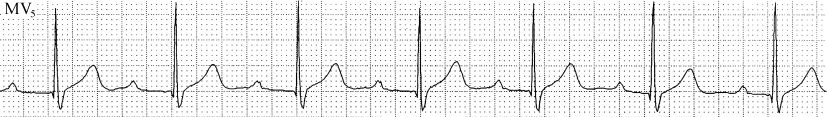
\includegraphics[width=5.58333in,height=0.78125in]{./images/Image00042.jpg}
 \captionsetup{justification=centering}
 \caption{反向一度Ⅰ型房室传导阻滞(P-R间期由0.38s缩短至0.30s)}
 \label{fig2-7}
  \end{figure} 

\begin{figure}[!htbp]
 \centering
 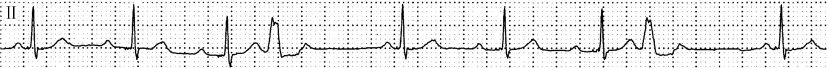
\includegraphics[width=5.58333in,height=0.45833in]{./images/Image00043.jpg}
 \captionsetup{justification=centering}
 \caption{室性早搏、3相性一度房室传导阻滞(代偿间歇后P-R间期由0.26s缩短至0.15s,但不能排除房室结内双径路传导)}
 \label{fig2-8}
  \end{figure} 

\begin{figure}[!htbp]
 \centering
 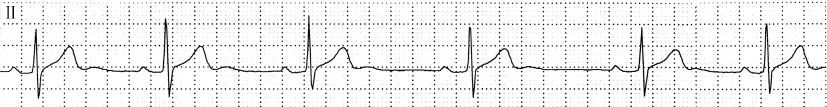
\includegraphics[width=5.58333in,height=0.71875in]{./images/Image00044.jpg}
 \captionsetup{justification=centering}
 \caption{窦性心动过缓伴不齐、4相性一度房室传导阻滞(P-R间期有0.20s、0.25s两种)}
 \label{fig2-9}
  \end{figure} 

(3)阻滞部位:一度房室传导阻滞部位可发生在心房内、房-结区、结区、结-希区、希氏束、双束支或三分支水平,其中以房室结内阻滞最为常见,约占90\%。希氏束电图能准确地判断房室传导阻滞的部位。体表心电图亦能初步诊断:①若P-R间期延长是由于P波时间明显增宽所致,且PR段时间正常,则阻滞部位多发生在心房或房-结区部位;②若仅PR段明显延长,则阻滞部位多发生在房室结内;③若P-R间期延长合并左束支阻滞,则阻滞部位绝大多数在双束支水平;④若P-R间期延长合并右束支阻滞,则阻滞部位在房室结内或双束支水平,各占50\%左右。

3.二度Ⅰ型、Ⅱ型房室传导阻滞

(1)典型的二度Ⅰ型房室传导阻滞:又称为房室文氏型阻滞或文氏现象,其P-R间期逐搏延长,直至P波受阻、QRS波群脱落,但每搏延长的增量逐渐缩短;R-R间期逐搏缩短,直至出现一个长R-R间期;长R-R间期小于任何短R-R间期的2倍(图\ref{fig2-10})。

(2)二度Ⅱ型房室传导阻滞:P-R间期固定(正常或延长),直至P波受阻、QRS波群脱落。

\begin{figure}[!htbp]
 \centering
 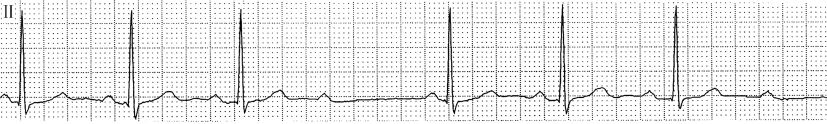
\includegraphics[width=5.58333in,height=0.83333in]{./images/Image00045.jpg}
 \captionsetup{justification=centering}
 \caption{二度Ⅰ型房室传导阻滞、房室呈4:3传导}
 \label{fig2-10}
  \end{figure} 

4.房室结内双径路传导

当快径路前向阻滞时,窦性激动沿着慢径路下传,出现P-R间期延长。诊断房室结内双径路传导,则要求P-P间期基本规则,出现长、短两种P-R间期且互差≥0.06s(图\ref{fig2-11})。

\begin{figure}[!htbp]
 \centering
 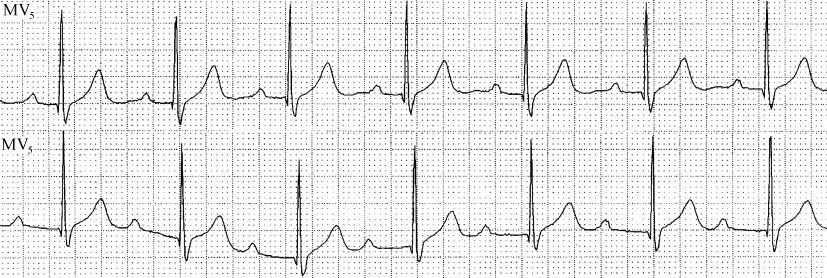
\includegraphics[width=5.58333in,height=1.875in]{./images/Image00046.jpg}
 \captionsetup{justification=centering}
 \caption{上、下两行系MV\textsubscript{5}}
 \label{fig2-11}
  \end{figure} 
导联同时不连续记录,显示一度房室传导阻滞、房室结内双径路传导(P-P间期规则时,其P-R间期有0.24s、0.38s两种)

5.干扰性P-R间期延长

(1)窦性早搏、房性早搏、干扰性房室分离时的窦性夺获、间位型室性早搏后第1个窦性搏动落在T波上,下传的P(P′)-R间期较长,且其P(P′)-R间期与R-P(P′)间期呈反比关系,即P(P′)-R间期长,其R-P(P′)间期短;反之,P(P′)-R间期短,其R-P(P′)间期长。若P(P′)波分别落在ST段、T波及TP段上,其下传的P(P′)-R间期呈固定地延长,则应考虑房室结内慢径路下传。

(2)窦性搏动遇及房室交接区隐匿性早搏的相对不应期,将引起个别心搏的P-R间期突然延长,但需有显性房室交接性早搏出现作为佐证。多见于房室交接区并行心律。

6.高度~几乎完全性房室传导阻滞时,出现超常期传导可引起P-R间期显著延长。

(二)临床意义

(1)P-R间期延长可见于心外因素,如抗心律失常药物、电解质紊乱(低钾、高钾血症)、迷走神经张力过高、颅脑损伤等,但更多见于急性心肌炎、心肌缺血、扩张型心肌病等器质性心脏病或功能性改变,如房室结内双径路传导等。大部分预后良好,可终身不变。

(2)突然发生或新发生的一度房室传导阻滞,需进一步查明原因和随访,警惕发展为高度或三度房室传导阻滞。

(3)P-R间期过度延长时(>0.35s),可发生P-R间期过度延长综合征。此时心室舒张期及有效充盈期均显著缩短而引起二尖瓣返流及心功能不全,可置入双腔起搏器;若由房室结慢径路下传者,可行射频消融术。

\protect\hypertarget{text00008.htmlux5cux23subid33}{}{}

\subsection{P-R间期长、短交替}

窦性心律时,出现P-R间期长、短交替,见于下列5种情况:

(1)房室交接区快、慢径路交替性传导:当P-P间期基本规则时,P-R间期呈长、短交替出现,且两者互差≥0.06s。

(2)交替性预激:短P-R间期者,QRS波群起始部有“δ”波,QRS波群时间增宽,ST-T呈继发性改变,其P-J间期与正常P-R间期、正常QRS波群的P-J间期相等。系房室旁道呈2:1阻滞所致(图\ref{fig2-12})。

\begin{figure}[!htbp]
 \centering
 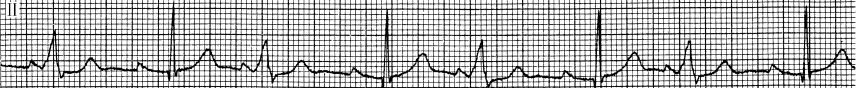
\includegraphics[width=5.78125in,height=0.59375in]{./images/Image00047.jpg}
 \captionsetup{justification=centering}
 \caption{一度房室传导阻滞、交替性A型预激综合征引起P-R间期长、短交替(与图\ref{fig2-5}系同一病例)}
 \label{fig2-12}
  \end{figure} 

(3)3:2房室文氏现象:文氏周期中,第2个搏动的P-R间期较第1个长,第3个搏动P波下传受阻,导致P-R间期长、短交替出现。

(4)房室结快、慢径路均呈3:1传导:第1个搏动由快径路下传,第2个搏动由慢径路下传,第3个搏动快、慢径路下传均受阻,导致P-R间期长、短交替出现(图\ref{fig2-13})。

\begin{figure}[!htbp]
 \centering
 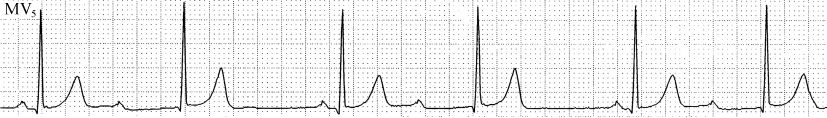
\includegraphics[width=5.58333in,height=0.79167in]{./images/Image00048.jpg}
 \captionsetup{justification=centering}
 \caption{房室结快、慢径路均呈3:1传导,引起P-R间期长、短交替(0.17s、0.47~0.53s)}
 \label{fig2-13}
  \end{figure} 

(5)舒张晚期室性早搏二联律:短P-R间期者,QRS波群宽大畸形,ST-T呈继发性改变,其P-J间期与正常P-R间期、正常QRS波群的P-J间期不等。

\protect\hypertarget{text00008.htmlux5cux23subid34}{}{}

\section{P-J间期}

P-J间期是指P波开始到J点结束,代表心房开始除极到心室除极结束所需的时间,包括P-R间期和QRS波群时间,正常值≤0.27s。当发生一度房室传导阻滞、束支阻滞、不定型心室内传导阻滞等心室除极时间延长时,则P-J间期>0.27s。P-J间期在预激综合征诊断和鉴别诊断中具有重要意义。

(1)间歇性预激综合征(不完全性预激)与舒张晚期室性早搏的鉴别:两者P-R间期均缩短,QRS波群时间均增宽,但前者的P-J间期与正常QRS波群的P-J间期相等,而后者则不相等。

(2)预激综合征P-J间期>0.27s时,多数合并束支阻滞,少数可能合并房室旁道一度阻滞或同时伴有正道一度、三度阻滞。P-J间期包括P-R间期与QRS波群时间,绝大多数预激综合征的P-J间期正常(≤0.27s)。因束支阻滞的P-J间期等于房室结传导时间+希浦系传导时间+束支阻滞部位的心室终末除极时间,故一般均>0.27s;而预激综合征合并束支阻滞的P-J间期等于房室旁道传导时间+希浦系传导时间+束支阻滞部位的心室终末除极时间。两者相比,后者的P-J间期较前者略短。当房室旁道下传时间与心室间及心室内传导时间的总和≥房室结传导时间与心室间及心室内传导时间的总和时,束支阻滞图形不会被掩盖,此时P-J间期延长(>0.27s)。房室旁道一度阻滞或同时伴有正道一度、三度阻滞,也将导致P-J间期>0.27s。

(3)不同部位预激综合征对P-J间期的影响:大多数预激综合征的P-J间期正常(≤0.27s),少数预激综合征(右后、右后间隔旁道)的P-J间期明显短于正常QRS波群的P-J间期,因P-J间期包括冲动从正道下传的房室传导时间和心室除极时间,旁道传导不影响冲动从正道下传的房室传导时间,但可缩短心室除极时间,故可引起P-J间期缩短,尤其是房室旁道位置靠近心室最后除极部位(心室后基底部)及δ波较大者。

\protect\hypertarget{text00009.html}{}{}

\protect\hypertarget{text00009.htmlux5cux23chapter9}{}{}

\chapter{正常QRS波群及其异常改变}

\protect\hypertarget{text00009.htmlux5cux23subid35}{}{}

\section{正常QRS波群}

\protect\hypertarget{text00009.htmlux5cux23subid36}{}{}

\subsection{QRS波群的命名}

QRS波群是室间隔、右心室和左心室电激动过程中所产生的除极波。第1个向下的波称为Q(q)波,最初1个向上的波称为R(r)波,R(r)波之后向下的波称为S(s)波,有时S波之后又出现1个向上的波,则称为R′(r′)波,之后再出现一个向下的波,称为S′(s′)波;若只有向下的波,而没有向上的波,称为QS波。当波幅≥0.5mV时,用Q、R、S表示;当波幅<0.5mV时,用q、r、s表示。

\protect\hypertarget{text00009.htmlux5cux23subid37}{}{}

\subsection{各波的正常值}

1.Q(q)波

正常q波时间<0.04s,深度<$\frac{1}{4}$
R。若其时间≥0.04s或(和)深度≥$\frac{1}{4}$
R,则称为异常Q波。

2.R波振幅

(1)肢体导联:①心脏呈横位型时,R\textsubscript{I} +S\textsubscript{Ⅲ}
<2.5mV,R\textsubscript{I} <1.5mV,R\textsubscript{aVL}
<1.2mV;②心脏呈悬位型时,R\textsubscript{Ⅱ、Ⅲ、aVF}
<2.0mV;③aVR导联Q/R>1,R<0.5mV;④所有肢体导联R+S>0.5mV。

(2)胸前导联:①R\textsubscript{V\textsubscript{1}}
<1.0mV,R\textsubscript{V\textsubscript{1}}
+S\textsubscript{V\textsubscript{5}} <1.2mV,V\textsubscript{1}
导联R/S<1.②建议国人采用男性R\textsubscript{V\textsubscript{5}}
、\textsubscript{V\textsubscript{6}}
<3.0mV、R\textsubscript{V\textsubscript{5}}
+S\textsubscript{V\textsubscript{1}}
<4.5mV;女性R\textsubscript{V\textsubscript{5}}
、\textsubscript{V\textsubscript{6}}
<2.8mV、R\textsubscript{V\textsubscript{6}}
+S\textsubscript{V\textsubscript{1}} <4.0mV,V\textsubscript{5}
、V\textsubscript{6} 导联R/S>1.③V\textsubscript{3}
导联R+S<6.0mV。④所有胸前导联R+S>1.0mV。

3.QRS波群时间

<4岁的儿童,QRS波群时间<0.09s;4~16岁者,QRS波群时间<0.10s;成年男性,QRS波群时间≤0.11s。“心电图标准化与解析的建议------2009年国际指南”(以下简称“2009年国际指南”)推荐≥16岁者,QRS波群时间>0.11s为异常。

\protect\hypertarget{text00009.htmlux5cux23subid38}{}{}

\section{QRS波群振幅异常改变}

\protect\hypertarget{text00009.htmlux5cux23subid39}{}{}

\subsection{低电压}

1.心电图特征

所有肢体导联R+S<0.5mV或胸前导联R+S<1.0mV。

2.临床意义

(1)心外因素:见于肺气肿、胸腔积液或积气、心包积液、过度肥胖、甲状腺功能减退等。

(2)心内因素:①心肌梗死:大面积心肌梗死者,出现低电压,提示预后不良;②扩张型心肌病;③心力衰竭。

(3)正常人群:约有1\%的正常人可出现低电压。

\protect\hypertarget{text00009.htmlux5cux23subid40}{}{}

\subsection{高电压}

1.右胸导联高电压

(1)右心室肥大。

(2)右束支阻滞:①V\textsubscript{1}
导联QRS波群呈rsR′型或M型;②其他导联终末S波或R波宽钝错折;③QRS波群时间>0.11s。

(3)Ⅱ型左中隔支阻滞:①V\textsubscript{1} 、V\textsubscript{2}
导联QRS波群呈Rs型,R/s>1;②V\textsubscript{5} 、V\textsubscript{6}
导联QRS波群呈Rs型或qRs型,其q波很小,时间<0.01s,深度<0.1mV;③R\textsubscript{V\textsubscript{2}}
>R\textsubscript{V\textsubscript{6}}
;④QRS波群时间正常(合并束支阻滞时除外);⑤多见于老年冠心病患者;⑥需排除右心室肥大、逆钟向转位、A型预激综合征、后壁心肌梗死等(图\ref{fig3-1})。

\begin{figure}[!htbp]
 \centering
 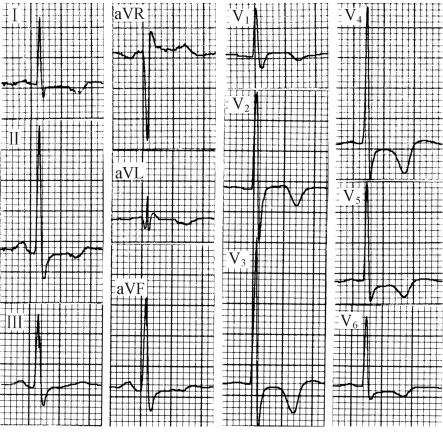
\includegraphics[width=2.98958in,height=2.91667in]{./images/Image00050.jpg}
 \captionsetup{justification=centering}
 \caption{V\textsubscript{1} ~V\textsubscript{6}}
 \label{fig3-1}
  \end{figure} 
导联定准电压为0.5mV,高血压病患者出现Ⅱ型左中隔支阻滞、左心室肥大伴劳损

(4)A、C型预激综合征(图\ref{fig3-2})。

\begin{figure}[!htbp]
 \centering
 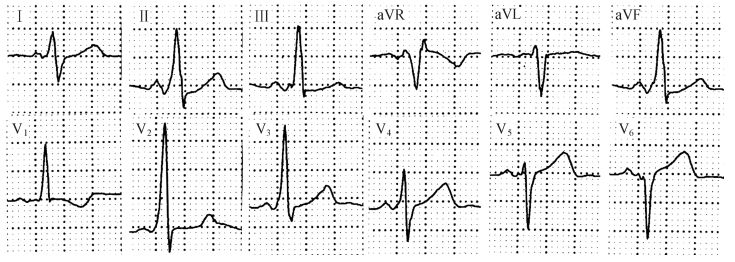
\includegraphics[width=4.96875in,height=1.77083in]{./images/Image00051.jpg}
 \captionsetup{justification=centering}
 \caption{心动过速患者体检时发现C型预激综合征}
 \label{fig3-2}
  \end{figure} 

(5)后壁心肌梗死:①V\textsubscript{3} R、V\textsubscript{1}
、V\textsubscript{2}
导联R波增高,呈Rs型伴ST段压低、T波高耸;②V\textsubscript{7}
、V\textsubscript{8}
导联出现异常Q波,呈QR、Qr、QS型伴ST段抬高、T波倒置。

(6)逆钟向转位:①V\textsubscript{1} ~V\textsubscript{3}
导联呈Rs型或RS型,R/S>1;②V\textsubscript{5} 、V\textsubscript{6}
呈qR、Rs型。

(7)右心室电压占优势:①见于婴幼儿、儿童;②心脏无病理性杂音;③电轴右偏;④V\textsubscript{1}
、V\textsubscript{2} 导联呈Rs型,R/s>1。

2.左胸导联、肢体导联高电压

(1)左心室高电压:①R\textsubscript{Ⅰ} +S\textsubscript{Ⅲ}
>2.5mV,R\textsubscript{aVL}
>1.2mV,见于横位型心脏、肥胖者;②R\textsubscript{Ⅱ、Ⅲ、aVF}
>2.0mV,见于悬位型心脏、瘦长型者;③男性R\textsubscript{V\textsubscript{5}}
+S\textsubscript{V\textsubscript{1}}
>4.5mV、女性R\textsubscript{V\textsubscript{5}}
+S\textsubscript{V\textsubscript{1}}
>4.0mV;④男性R\textsubscript{V\textsubscript{5}}
、\textsubscript{V\textsubscript{6}}
>3.0mV、女性R\textsubscript{V\textsubscript{5}}
、\textsubscript{V\textsubscript{6}} >2.8mV;⑤男性R\textsubscript{aVL}
+S\textsubscript{V\textsubscript{3}} >2.8mV、女性R\textsubscript{aVL}
+S\textsubscript{V\textsubscript{3}} >2.0mV。

(2)左心室肥大。

3.左、右胸导联均为高电压

(1)A型预激综合征。

(2)双心室肥大。

(3)左心室肥大伴逆钟向转位。

(4)左心室肥大合并Ⅱ型左中隔支阻滞(图\ref{fig3-1})。

\protect\hypertarget{text00009.htmlux5cux23subid41}{}{}

\subsection{右心室肥大}

在正常情况下,左心室壁较右心室壁约厚3倍。轻度右心室肥大所增加的向右前向量往往被左心室除极向量所抵消,其肥大的图形被掩盖。只有右心室显著肥大,且其心室壁厚度大于左心室时,才表现出右心室肥大的心电图特征。

1.心电图特征

(1)电轴右偏>+110°,R\textsubscript{Ⅲ} >R\textsubscript{aVF} 。

(2)aVR导联呈QR型,Q/R<1,R波幅>0.5mV。

(3)V\textsubscript{1} 导联呈qR、qRs、R、Rs、rsR′(R′波不宽钝)型。

(4)V\textsubscript{5} 、V\textsubscript{6} 导联呈RS型,R/S<1.

(5)出现肺型P波及V\textsubscript{1} ~V\textsubscript{6}
导联均呈rS型,r/S<1,多见于肺心病。

(6)V\textsubscript{1} ~V\textsubscript{3}
导联可有ST段压低,T波呈负正双向或倒置(图\ref{fig3-3})。

\begin{figure}[!htbp]
 \centering
 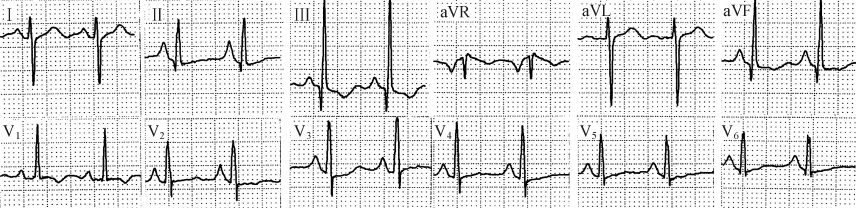
\includegraphics[width=5.78125in,height=1.40625in]{./images/Image00052.jpg}
 \captionsetup{justification=centering}
 \caption{法洛四联症患者出现右心房、右心室肥大、下壁及前侧壁轻度T波改变}
 \label{fig3-3}
  \end{figure} 

2.根据心电图特征分型

(1)轻度肥大:电轴轻度右偏、V\textsubscript{1}
导联呈rsR′型,V\textsubscript{2} ~V\textsubscript{6}
导联均呈rS型。多见于房间隔缺损、肺源性心脏病等。

(2)中度肥大:电轴中度右偏、V\textsubscript{1}
导联呈Rs或RS型、V\textsubscript{5} 、V\textsubscript{6}
呈RS或rS型。多见于室间隔缺损、风心病二尖瓣狭窄等。

(3)重度肥大:电轴重度右偏,V\textsubscript{1}
导联呈qR、qRs、R型,V\textsubscript{5} 、V\textsubscript{6}
导联呈rS型。多见于法洛四联症、肺动脉瓣狭窄等。

3.根据右心室负荷过重情况分型

(1)收缩期负荷过重型:系右心室射血时阻力增加,心肌发生代偿性肥厚所致。V\textsubscript{1}
导联QRS波群呈qR、qRs、R、Rs型;V\textsubscript{1} ~V\textsubscript{3}
导联ST段压低、T波倒置。多见于法洛四联症、肺动脉瓣狭窄。

(2)舒张期负荷过重型:右心室回心血量增多,使右心室舒张期负荷增加而扩张。V\textsubscript{1}
导联QRS波群呈rsR′型。多见于房间隔缺损等。

4.右心室肥大合并右束支阻滞

右心室压力增高导致右心室肥大,易伤及右束支使其阻滞。表现为QRS波群时间≥0.12s,电轴右偏,aVR导联R波增宽、增高,Ⅰ、aVL、V\textsubscript{5}
、V\textsubscript{6} 导联S波增宽。

\protect\hypertarget{text00009.htmlux5cux23subid42}{}{}

\subsection{左心室肥大}

1.心电图特征

(1)有左心室高电压的心电图表现。

(2)QRS波群时间轻度增宽(0.10~0.12s)。

(3)电轴轻、中度左偏(+30°~-30°)。

(4)以R波为主导联出现轻度ST段压低(<0.1mV)、T波低平,系继发性ST-T改变。

(5)有引起左心室肥大的临床依据。

2.根据心肌肥厚部位、心腔大小分型

(1)向心性肥厚:心室壁增厚,心腔不扩大。

(2)离心性肥厚:心腔扩大,心室腔与心室壁的比值不增加。

(3)扩张型心室肥厚:心腔不成比例增大,心室壁与心室腔比值缩小,心脏重量增加。

(4)非对称性流出道狭窄。

3.根据左心室负荷过重分型

(1)收缩期负荷过重型:系左心室射血时阻力增加,心肌发生代偿性向心性肥厚。左胸导联R波振幅增高伴ST段压低、T波低平或倒置。多见于高血压病、主动脉瓣狭窄及梗阻型肥厚性心肌病等。

(2)舒张期负荷过重型:系左心室回心血量增多,使左心室舒张期负荷增加而扩张,为离心性或扩张型心室肥厚。左胸导联R波振幅增高伴ST段抬高、T波高耸。多见于二尖瓣关闭不全、主动脉瓣关闭不全等。

4.左心室肥大伴劳损

有左心室肥大的心电图特征,同时伴有原发性ST-T改变,即ST段呈下斜型、水平型压低(≥0.1mV),T波倒置或负正双向以负为主,可伴有U波倒置(图\ref{fig3-4})。“2009年国际指南”指出不再应用“劳损”,而改称为“继发性ST-T改变”,本人持有异议。

\begin{figure}[!htbp]
 \centering
 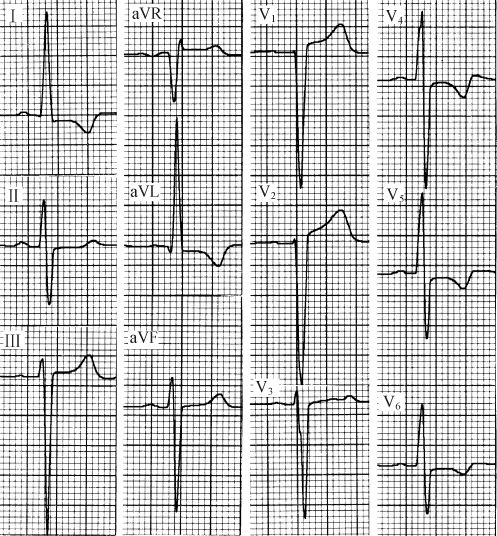
\includegraphics[width=3.35417in,height=3.625in]{./images/Image00053.jpg}
 \captionsetup{justification=centering}
 \caption{主动脉瓣狭窄患者出现左心室肥大伴劳损、左前分支阻滞(定准电压均为0.5mV)}
 \label{fig3-4}
  \end{figure} 

5.左心室劳损

有左心室肥大的临床依据,但心电图QRS波群振幅正常,仅出现原发性ST-T改变者,可伴有U波倒置,称为左心室劳损。

\protect\hypertarget{text00009.htmlux5cux23subid43}{}{}

\subsection{双心室肥大}

1.双心室肥大的心电图表现形式

(1)心电图正常或大致正常。

(2)仅有QRS波群时间轻度增宽及轻度ST-T改变。

(3)仅显示左心室肥大的心电图改变,此时右心室呈轻、中度肥大。

(4)仅显示右心室肥大的心电图改变,此时右心室显著肥大。

(5)同时显示双心室肥大的心电图改变,左、右胸导联R波振幅均增高。

2.有明确的左心室肥大的心电图特征,同时伴有下列一项或几项改变者,应提示双心室肥大

(1)电轴右偏(>+110°,图\ref{fig3-5})。

\begin{figure}[!htbp]
 \centering
 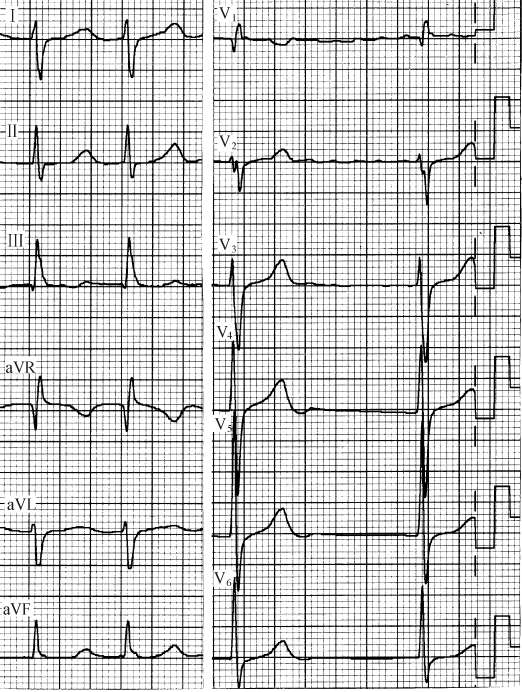
\includegraphics[width=3.52083in,height=4.67708in]{./images/Image00054.jpg}
 \captionsetup{justification=centering}
 \caption{风心病、二尖瓣狭窄伴关闭不全,定准电压均为0.5mV。显示心房颤动、左心室肥大(R\textsubscript{V\textsubscript{5}}}
 \label{fig3-5}
  \end{figure} 
电压4.0mV)、电轴右偏(+120°)(提示双心室肥大)、不完全性右束支阻滞

(2)aVR导联Q/R<1,R>0.5mV。

(3)V\textsubscript{1} 导联呈Rs型,R/s>1或呈R型。

(4)显著的顺钟向转位,V\textsubscript{5} 、V\textsubscript{6}
导联有深的S波。

(5)出现肺型P波,系右心房肥大所致(图\ref{fig3-6})。

\begin{figure}[!htbp]
 \centering
 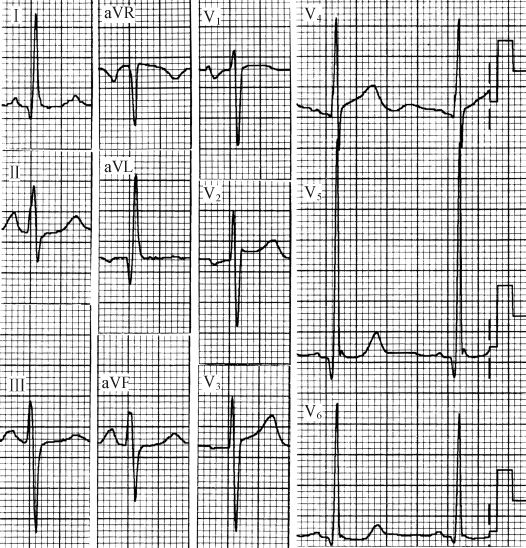
\includegraphics[width=3.55208in,height=3.69792in]{./images/Image00055.jpg}
 \captionsetup{justification=centering}
 \caption{风心病、双瓣膜病变患者心电图出现左心室、右心房肥大(定准电压均为0.5mV,心脏超声波、胸片均显示全心扩大)}
 \label{fig3-6}
  \end{figure} 

3.有明确的右心室肥大的心电图特征,同时伴有下列一项或几项改变者,应提示双心室肥大

(1)电轴左偏。

(2)V\textsubscript{5} 、V\textsubscript{6}
导联R波振幅>2.5mV伴ST-T改变。

(3)V\textsubscript{3} 导联R+S>6.0mV,R/S≈1.

(4)男性R\textsubscript{aVL} +S\textsubscript{V\textsubscript{3}}
>2.8mV、女性R\textsubscript{aVL} +S\textsubscript{V\textsubscript{3}}
>2.0mV。

(5)R\textsubscript{Ⅰ} +S\textsubscript{Ⅲ}
>2.5mV,R\textsubscript{aVL} >1.2mV。

\protect\hypertarget{text00009.htmlux5cux23subid44}{}{}

\subsection{心室肥厚、扩大、肥大的区别}

1.心室肥厚:主要指心肌细胞增粗、增长所致心室壁厚度增加、重量增加,但心室腔容积不增大。

2.心室扩大:主要指心室腔的容积增大,可伴有轻度心室壁增厚。

3.心室肥大:肥厚与扩大均兼有之。病程较久的病例,无论是收缩期负荷过重,还是舒张期负荷过重,往往存在着不同程度的心室壁增厚和心腔容积增大,故本人主张用“心室肥大”一词。

\protect\hypertarget{text00009.htmlux5cux23subid45}{}{}

\subsection{异常Q波}

1.异常Q波

(1)Q波时间≥0.04s。

(2)Q波深度≥$\frac{1}{4}$ R。

(3)呈QS型,起始部错折或呈QrS、Qrs或qrS型(该r波又称为胚胎型r波)。

2.等位性Q波(属异常Q波范畴)

(1)原无q波的导联上突然出现了q波伴ST段损伤型抬高。

(2)以R波为主导联,其R波振幅较原来显著降低伴ST段损伤型抬高。

(3)V\textsubscript{1} ~V\textsubscript{4}
导联r(R)波振幅逐渐降低,呈逆递增现象。

(4)V\textsubscript{1} ~V\textsubscript{4}
导联r(R)波振幅递增不良:相邻两个导联的r(R)波振幅递增量<0.1mV。

(5)不应该出现Q(q)波的导联出现了Q(q)波,如V\textsubscript{1}
、V\textsubscript{2} 导联呈qrS型,或V\textsubscript{3}
、V\textsubscript{4} 导联出现q波而V\textsubscript{5}
、V\textsubscript{6} 导联无q波,或V\textsubscript{3}
、V\textsubscript{4} 导联q波深度>V\textsubscript{5}
、V\textsubscript{6} 导联q波深度。

(6)镜像改变,如V\textsubscript{1} 、V\textsubscript{2}
导联R波振幅增高,而V\textsubscript{7} 、V\textsubscript{8}
导联出现异常Q波。

(7)左束支阻滞时,Ⅰ、aVL、V\textsubscript{5} 、V\textsubscript{6}
导联呈qR型。

3.引起异常Q波的常见原因

(1)急性心肌梗死引起心肌细胞组织学上坏死或电学上的电静止。

(2)陈旧性心肌梗死或心肌病患者出现心肌纤维化。

(3)显著右心室肥大导致心脏顺钟向转位,使Ⅰ、aVL导联或V\textsubscript{1}
、V\textsubscript{2} 导联呈QS型、qR型。

(4)Ⅰ型左中隔支阻滞导致V\textsubscript{1} 、V\textsubscript{2}
导联呈qR、QR、qrS或QS型。只有间歇性出现时,方能诊断(图\ref{fig21-9})。

(5)预激综合征时“δ”波呈负相时,可使不同导联出现异常Q波。

4.高侧壁(Ⅰ、aVL导联)出现异常Q波

(1)高侧壁或广泛前壁心肌梗死。

(2)预激向量指向右下方的预激综合征。

(3)显著的右心室肥大。

(4)右位心。

5.下壁(Ⅱ、Ⅲ、aVF导联)出现异常Q波

(1)下壁心肌梗死。

(2)左束支阻滞合并显著的电轴左偏:Ⅱ、Ⅲ、aVF导联可呈QS型,Ⅲ导联QS波深度大于Ⅱ导联QS波深度。

(3)预激向量指向左上方的预激综合征。

(4)二尖瓣脱垂:①Ⅱ、Ⅲ、aVF导联可呈QS型,且出现ST段压低、T波倒置;②听诊有喀喇音;③超声心动图显示二尖瓣脱垂的特征性改变。

6.右胸导联(V\textsubscript{1} 、V\textsubscript{2} 导联)出现异常Q波

(1)前间壁心肌梗死。

(2)室间隔肥厚性心肌病导致心肌纤维化。

(3)左束支阻滞。

(4)Ⅰ型左中隔支阻滞:V\textsubscript{1} 、V\textsubscript{2}
导联呈qR、QR、qrS或QS型,需排除右心室肥大、前间壁心肌梗死、前间壁心肌纤维化及B型预激综合征。间歇性出现上述波形时,能明确诊断。

(5)肺气肿、肺心病。

(6)显著的右心室肥大。

(7)B型预激综合征。

(8)部分左心室肥大伴劳损。

(9)左前分支阻滞。

7.左胸导联(V\textsubscript{4} 、V\textsubscript{5} 、V\textsubscript{6}
导联)出现异常Q波

(1)前壁或前侧壁心肌梗死。

(2)肥厚性梗阻型心肌病出现深而窄的Q波。

(3)左心室舒张期负荷过重导致左心室肥大时,可出现深而窄的Q波。

(4)C型预激综合征。

(5)右位心。

\protect\hypertarget{text00009.htmlux5cux23subid46}{}{}

\subsection{QRS波群电交替、电阶梯现象}

1.基本概念

(1)QRS波群电交替现象:系指源自同一起搏点的心搏(多为窦性节律),在排除2:1分支阻滞及心外因素影响下,其QRS波群时间不变,仅波形或(和)波幅每搏呈交替性改变。可同时伴有其他波、段的电交替。

(2)QRS波群电阶梯现象:系一种特殊的电交替现象,指源自同一起搏点的心搏(多为窦性节律),在排除心外因素影响及分支内文氏现象下,其QRS波群时间不变,仅波形或(和)波幅由浅→深→浅或由低→高→低,周而复始,有规律地演变。可同时伴有ST段、T波的电阶梯现象。

2.心电图特征

(1)QRS波群电交替现象:①心搏来源恒一,多为窦性节律;②QRS波群时间固定不变;③任何导联上QRS波幅相差≥0.1mV,以胸前导联为多见,尤以V\textsubscript{2}
、V\textsubscript{3}
导联最常见;④心率增快时(>100次/min),尤其是阵发性心动过速时更易出现,为快频率依赖性电交替;⑤与束支、分支阻滞无关,与心外因素无关,如呼吸、体位、胸腔积液等;⑥若同时伴有≥2个其他波、段的电交替,则称为完全性电交替现象(图\ref{fig3-7}、图\ref{fig3-8})。

\begin{figure}[!htbp]
 \centering
 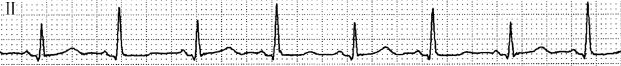
\includegraphics[width=4.19792in,height=0.4375in]{./images/Image00056.jpg}
 \captionsetup{justification=centering}
 \caption{QRS波群、T波电交替现象}
 \label{fig3-7}
  \end{figure} 

\begin{figure}[!htbp]
 \centering
 \includegraphics[width=5.78125in,height=1.17708in]{./images/Image00057.jpg}
 \captionsetup{justification=centering}
 \caption{阵发性室上性心动过速出现QRS波群、T波电交替现象}
 \label{fig3-8}
  \end{figure} 

(2)QRS波群电阶梯现象:①心搏来源恒一,多为窦性节律;②QRS波群时间固定不变;③任何导联上QRS波形或(和)波幅由浅→深→浅或由低→高→低,振幅相差≥0.1mV,周而复始,有规律地演变;④与束支、分支阻滞无关,与心外因素无关,如呼吸、体位、胸腔积液等;⑤可同时伴有ST段、T波的电阶梯现象(图\ref{fig3-9})。

\begin{figure}[!htbp]
 \centering
 \includegraphics[width=5.78125in,height=0.51042in]{./images/Image00058.jpg}
 \captionsetup{justification=centering}
 \caption{加速的房性逸搏心律伴James束下传(P-R间期0.08s)、QRS波群电阶梯现象}
 \label{fig3-9}
  \end{figure} 

3.发生机制

(1)多与心肌、传导组织不同程度的缺血、缺氧引起不应期延长,导致心肌细胞除极、复极不完全有关,尤其是心室率过快导致心室舒张期明显缩短时。

(2)顺向型房室折返性心动过速时,其QRS波群电交替发生率较高,这与冲动在传导组织内发生交替性功能性传导延缓有关。

4.临床意义

(1)QRS波群电交替可见于大量心包积液或心包填塞、严重的心肌病变,如冠心病、心肌梗死、扩张型心肌病等。若发生在心率缓慢时,则提示心肌病变严重,预后较差;若发生在心动过速时,则无特别临床意义,随着心动过速的终止,QRS波群电交替自行消失。

(2)窄QRS心动过速伴有QRS波群电交替,对判断顺向型房室折返性心动过速具有高度的特异性(96\%)。

(3)宽QRS心动过速伴QRS波群电交替者,多有合并房室旁道传导。

(4)QRS波群电阶梯现象多见于严重的器质性心脏病、高钾血症等,提示心肌病变严重而广泛,预后较差,但与原发病有关。

\protect\hypertarget{text00009.htmlux5cux23subid47}{}{}

\section{QRS波群电轴偏移}

\protect\hypertarget{text00009.htmlux5cux23subid48}{}{}

\subsection{电轴测量方法及其分类标准}

1.电轴测量方法

通常测量额面心电轴。根据肢体六个导联QRS波群振幅的高低,可用目测法进行初步评估电轴是左偏、右偏还是不偏;而用振幅查表法,则能较准确地求出电轴偏移的度数。

(1)粗略的目测法:根据Ⅰ、Ⅲ(或aVF)导联QRS主波方向加以判断,因Ⅰ、aVF导联轴的夹角为90°,故以Ⅰ、aVF导联目测心电轴较为恰当:①Ⅰ、Ⅲ(或aVF)导联QRS主波均向上,电轴正常;②Ⅰ导联QRS主波向上,Ⅲ(或aVF)导联QRS主波向下(又称为背道而驰),电轴左偏;③Ⅰ导联QRS主波向下,Ⅲ(或aVF)导联QRS主波向上(又称为针锋相对),电轴右偏;④Ⅰ、Ⅲ(或aVF)导联QRS主波均向下,电轴极度右偏(又称为无人区电轴)。

(2)较为精确的目测法:要求熟悉六轴系统各个导联轴所在的位置与角度。找出R波振幅最高和次高的导联,则电轴就位于这两个导联轴之间,且偏向波幅最高的导联轴。若最高和次高导联QRS波幅相等时,则电轴就位于这两个导联轴的中间。这种方法一般误差在5°以内。例如,Ⅱ导联(+60°)R波振幅最高,aVF导联(+90°)次高,则电轴位于+60°~+90°之间偏向+60°,约在+65°~+70°;若Ⅱ、aVF导联R波振幅最高,且相等时,则电轴位于+60°~+90°中间,即+75°左右。

(3)查表法:根据Ⅰ和Ⅲ导联QRS波幅的代数和进行查表,有2种方法:①计算QRS波群正相波振幅最高与负相波最深的代数和,如R-S或R-Q,其方法简便,也更为精确;②计算QRS波群所有向上和向下各波幅的代数和,如(R+R′)-(Q+S)。

2.分类标准

(1)目前国内常用标准:①+30°~+90°,电轴正常;②+30°~0°,电轴轻度左偏;③0°~-30°,电轴中度左偏;④-30°~-90°,电轴重度左偏;⑤+90°~+120°,电轴轻度右偏;⑥+120°~+180°,电轴中度右偏;⑦+180°~-90°,电轴重度右偏。

(2)世界卫生组织推荐的标准:①-30°~+90°,电轴正常;②-30°~-90°,电轴左偏;③+90°~+180°,电轴右偏;④-90°~+180°,电轴不确定。

(3)“2009年国际指南”的标准:①-30°~+90°,电轴正常;②-30°~-45°,中度左偏;③-45°~-90°,显著左偏;④+90°~+120°,中度右偏;⑤+120°~+180°,显著右偏。

\protect\hypertarget{text00009.htmlux5cux23subid49}{}{}

\subsection{电轴偏离的临床意义}

(1)电轴轻度左偏、右偏:多属于正常变异。

(2)电轴中、重度左偏:见于左前分支阻滞、左心室肥大、原发孔型房间隔缺损、预激综合征、横位型心脏等。

(3)电轴中度右偏:见于左后分支阻滞、右心室肥大、高侧壁心肌梗死等。

(4)电轴重度右偏或不确定者:又称为假性电轴左偏或无人区电轴。窦性心律时见于重度右心室肥大、S\textsubscript{Ⅰ}
S\textsubscript{Ⅱ} S\textsubscript{Ⅲ}
综合征、右心室内传导延缓等;宽QRS波群时见于室性早搏、室性心动过速,具有很高的特异性。

\protect\hypertarget{text00009.htmlux5cux23subid50}{}{}

\subsection{真性、假性电轴左偏的鉴别}

假性电轴左偏与真性电轴左偏的鉴别,见表3-1所示。

\begin{table}[htbp]
\centering
\caption{假性电轴左偏与真性电轴左偏的鉴别}
\label{tab3-1}
\includegraphics[width=5.46875in,height=1.51042in]{./images/Image00059.jpg}
\end{table}

\protect\hypertarget{text00009.htmlux5cux23subid51}{}{}

\subsection{S\textsubscript{Ⅰ} S\textsubscript{Ⅱ} S\textsubscript{Ⅲ} 综合征}

1.基本概念

S\textsubscript{Ⅰ} S\textsubscript{Ⅱ} S\textsubscript{Ⅲ}
综合征是指Ⅰ、Ⅱ、Ⅲ导联QRS波群同时存在明显的S波,其深度>0.3mV,且S\textsubscript{Ⅱ}
>S\textsubscript{Ⅲ} ,又称为3S综合征。

2.心电图特征

(1)Ⅰ、Ⅱ、Ⅲ导联QRS波群中均有明显的S波。

(2)S波振幅>0.3mV。

(3)S\textsubscript{Ⅱ} >S\textsubscript{Ⅲ} 。

(4)aVR导联Q/R<1,R>0.5mV。

(5)V\textsubscript{5} 、V\textsubscript{6}
导联呈RS型,R/S<1或S>$\frac{1}{2}$
R,呈高度顺钟向转位。

(6)上述心电图一旦出现,常持续存在(图\ref{fig3-10})。

\begin{figure}[!htbp]
 \centering
 \includegraphics[width=5.1875in,height=2.14583in]{./images/Image00060.jpg}
 \captionsetup{justification=centering}
 \caption{S\textsubscript{Ⅰ} S\textsubscript{Ⅱ} S\textsubscript{Ⅲ}}
 \label{fig3-10}
  \end{figure} 
综合征、顺钟向转位

3.临床意义

(1)正常变异:可见于少数正常人,尤其是瘦长无力型的人群中,与右心室传导延缓有关。

(2)右心室肥大:各种病因引起的严重右心室肥大,特别是右心室漏斗部、右心室流出道肥厚出现右心室电势占优势时,容易出现典型的S\textsubscript{Ⅰ}
S\textsubscript{Ⅱ} S\textsubscript{Ⅲ} 综合征。

(3)心肌梗死:各部位的心肌梗死,尤其是心尖部梗死更易出现典型的S\textsubscript{Ⅰ}
S\textsubscript{Ⅱ} S\textsubscript{Ⅲ} 综合征。

(4)脊柱畸形:多见于直背综合征患者。

\protect\hypertarget{text00009.htmlux5cux23subid52}{}{}

\subsection{左前分支阻滞}

1.心电图特征

(1)Ⅰ、aVL导联QRS波群呈qR型,R\textsubscript{aVL}
>R\textsubscript{Ⅰ、aVR} ,Ⅱ、Ⅲ、aVF导联呈rS型,S\textsubscript{Ⅲ}
>S\textsubscript{Ⅱ} >r\textsubscript{Ⅱ} 。

(2)心电轴左偏>-45°,有的学者认为心电轴左偏>-30°,即可诊断。

(3)V\textsubscript{1} ~V\textsubscript{6}
导联R波振幅降低,V\textsubscript{3} ~V\textsubscript{6}
导联S波加深呈RS型,有时V\textsubscript{1} 、V\textsubscript{2}
导联出现q波,呈qrS型。

(4)QRS波群时间正常(图\ref{fig3-11})。

\begin{figure}[!htbp]
 \centering
 \includegraphics[width=3.84375in,height=1.8125in]{./images/Image00061.jpg}
 \captionsetup{justification=centering}
 \caption{左前分支阻滞及V\textsubscript{5} 、V\textsubscript{6}}
 \label{fig3-11}
  \end{figure} 
导联S波加深

2.临床意义

左前分支阻滞约85\%由冠心病引起。此外,左心室肥大常合并左前分支阻滞。

\protect\hypertarget{text00009.htmlux5cux23subid53}{}{}

\subsection{左后分支阻滞}

1.心电图特征

(1)Ⅰ、aVL导联QRS波群呈rS型,S\textsubscript{aVL} >S\textsubscript{Ⅰ}
,Ⅱ、Ⅲ、aVF导联呈qR型,RⅢ>R\textsubscript{Ⅱ} 。

(2)心电轴右偏>+110°。若出现交替性或间歇性电轴右偏,又具有左后分支阻滞特征,即使未达到+110°,亦可诊断为左后分支阻滞。

(3)QRS波群时间正常。

(4)需排除右心室肥大、侧壁心肌梗死、悬位型心脏等。

2.临床意义

左后分支阻滞的发生率远低于左前分支阻滞。但一旦出现,则提示病变较广泛而严重。

\protect\hypertarget{text00009.htmlux5cux23subid54}{}{}

\section{QRS波群时间、形态异常改变}

\protect\hypertarget{text00009.htmlux5cux23subid55}{}{}

\subsection{左束支传导阻滞}

1.心电图特征

(1)V\textsubscript{1} 、V\textsubscript{2}
导联QRS波群呈rS型或QS型,V\textsubscript{5} 、V\textsubscript{6}
导联呈R型,R波平顶、挫折。

(2)Ⅰ、aVL导联QRS波群可呈R型或rS型,Ⅱ、Ⅲ、aVF导联可呈rS型或R型、qR型,心电轴可正常、左偏或右偏。

(3)QRS波群时间≥0.12s,多数达0.16s左右。

(4)ST-T方向多数与QRS主波方向相反,呈继发性改变。

(5)若QRS波群时间≥0.12s,则为完全性左束支传导阻滞;若QRS波群时间0.10~0.11s,则为不完全性左束支传导阻滞,但较罕见(图\ref{fig3-12})。

\begin{figure}[!htbp]
 \centering
 \includegraphics[width=5.58333in,height=2.29167in]{./images/Image00062.jpg}
 \captionsetup{justification=centering}
 \caption{不完全性左束支传导阻滞(QRS波群时间0.11~0.12s)}
 \label{fig3-12}
  \end{figure} 

2.临床意义

(1)绝大多数左束支传导阻滞见于器质性心脏病,如冠心病、心肌梗死、扩张型心肌病、高血压性心脏病等。

(2)常掩盖心肌梗死、心肌缺血、左心室肥大的心电图特征,易漏诊之。

(3)45岁以上发生左束支传导阻滞,其猝死的发生率为无束支传导阻滞者的10倍。

(4)若同时伴有一度、二度房室传导阻滞,则预后多严重,应及时安装人工起搏器。

\protect\hypertarget{text00009.htmlux5cux23subid56}{}{}

\subsection{右束支传导阻滞}

1.心电图特征

(1)V\textsubscript{1} 导联QRS波群多呈rS(s)R′型,ST段压低,T波倒置。

(2)其他导联QRS终末波宽钝、错折。

(3)QRS波群时间≥0.10s,电轴正常。若QRS波群时间≥0.12s,则为完全性右束支传导阻滞;若QRS波群时间0.10~0.11s,则为不完全性右束支传导阻滞。

(4)部分患者V\textsubscript{1}
导联QRS波群可出现以下变异:①呈R型或M型;②呈qR型,多见于合并前间壁、广泛前壁心肌梗死及重度右心室肥大时;③呈rS型,而V\textsubscript{2}
呈rS(s)R′型,见于右位心合并右束支传导阻滞;④呈rS或RS型,S波错折,加做V\textsubscript{3}
R导联呈rS(s)R′或rS(s)r′型,见于逆钟向转位、隐匿性不完全性右束支传导阻滞。

2.V\textsubscript{1} 导联QRS波群呈rS(s)R′(r′)型的常见原因

V\textsubscript{1}
导联QRS波群呈rS(s)R′(r′)型,时间≤0.11s,见于下列情况:

(1)正常变异:r′波系右心室流出道,尤其是室上嵴部位除极所致,r′<r波,当低一肋记录时,r′波可消失。Troudfit提出V\textsubscript{1}
导联r波幅<0.8mV,r′波幅<0.6mV,r′/S<1,属正常变异。

(2)右心室肥大:常见于房间隔缺损、室间隔缺损等右心室舒张期负荷过重患者,与中度右心室肥大有关。R′(r′)波及其他导联终末波无明显宽钝。

(3)不完全性右束支传导阻滞:R′(r′)波及其他导联终末波宽钝、错折。

(4)右心室肥大合并不完全性右束支传导阻滞:R′波及其他导联终末波宽钝、错折,R′>1.0mV,伴电轴右偏,V\textsubscript{5}
、V\textsubscript{6} 导联R/S<1或出现肺型P波。

(5)急性右心室扩张:急性肺栓塞时导致右心室扩张,心电图一过性出现V\textsubscript{1}
导联呈rS(s)R′(r′)型,肢体导联呈S\textsubscript{I} Q\textsubscript{Ⅲ}
、肺型P波和T波倒置。

(6)后壁心肌梗死:多数V\textsubscript{1}
导联QRS波群呈R型伴T波高耸,偶尔亦呈rS(s)r′型伴T波高耸。

3.临床意义

(1)传统的观点认为右束支传导阻滞多无重要临床意义,现发现多数右束支传导阻滞是有病因可寻的,往往是心脏疾病的早期表现。

(2)引起右束支传导阻滞最常见的病因有冠心病、心肌炎、心肌病、先天性心脏病等。

\protect\hypertarget{text00009.htmlux5cux23subid57}{}{}

\subsection{不定型心室内传导阻滞}

1.心电图特征

(1)QRS波形不符合左、右束支传导阻滞图形的特征。

(2)QRS波群时间≥0.12s。若QRS波群时间≥0.16s,则称为特宽型QRS波群(图\ref{fig3-13})。

\begin{figure}[!htbp]
 \centering
 \includegraphics[width=2.71875in,height=4.53125in]{./images/Image00063.jpg}
 \captionsetup{justification=centering}
 \caption{扩张型心肌病、全心扩大患者出现左前分支传导阻滞、不定型心室内传导阻滞、前壁r波振幅逆递增}
 \label{fig3-13}
  \end{figure} 

2.临床意义

多见于冠心病、扩张型心肌病、高钾血症、心力衰竭、药物中毒等。阻滞部位在浦肯野纤维、心室肌内。QRS波群愈宽,则提示心肌病变愈广泛和严重,预后愈差。

\protect\hypertarget{text00009.htmlux5cux23subid58}{}{}

\subsection{预激综合征}

1.典型预激综合征(W-P-W综合征)

P-R间期缩短,有“δ”波,QRS波群时间增宽,P-J间期≤0.27s及继发性ST-T改变。

2.变异型预激综合征(传统的Mahaim纤维预激综合征)

传统的Mahaim纤维又称为结-室旁道、束-室旁道。多位于右心室,QRS波形呈左束支阻滞图形。心电图特征:①P-R间期正常或延长(合并一度房室传导阻滞时);②有“δ”波;③QRS波群呈左束支阻滞图形,时间增宽,但<0.15s;④Ⅰ导联QRS波群呈R型,Ⅲ导联呈rS型,电轴左偏(0~-75°);⑤胸前导联QRS主波由向下转为向上的过渡区在V\textsubscript{4}
导联之后;⑥有继发性ST-T改变。

\protect\hypertarget{text00009.htmlux5cux23subid59}{}{}

\subsection{心室内差异性传导}

(一)时相性心室内差异性传导

它的发生与冲动提早出现有关,即通常所说的心室内差异性传导。

1.心电图特征

(1)提早出现室上性冲动,其下传QRS波群宽大畸形,时间<0.14s。其心电图特征:①室上性冲动指窦性早搏、窦房交接性早搏、房性早搏、房室交接性早搏、房室分离时窦性夺获、各类反复搏动、心房扑动、心房颤动、房性心动过速、房室交接性心动过速等;②宽大畸形QRS波群可呈右束支传导阻滞型(75\%~85\%)、左束支传导阻滞型(20\%~40\%)、右束支传导阻滞型加左前分支传导阻滞型(约18\%)、右束支传导阻滞型加左后分支传导阻滞型(约10\%)、单纯左前分支传导阻滞型(约33\%)、单纯左后分支传导阻滞型(约19\%)、左中隔支传导阻滞型及不定型心室内传导阻滞型。后两者少见。

(2)QRS波形易变性大,可呈完全性或不完全性束支、分支传导阻滞型。

(3)长-短周期后易出现心室内差异性传导,称为Ashman现象。

(4)偶见室性早搏伴心室内差异性传导,多发生在收缩中、晚期的同源性室性早搏,少数可发生在舒张早期。因遇及浦肯野纤维或心室肌的相对不应期而出现心室内差异性传导,其QRS波形较舒张期出现的室性早搏宽大畸形(图\ref{fig11-22})。

2.发生机制

(1)提早出现的室上性冲动下传心室时,束支、分支等传导组织生理性不应期尚未完全恢复正常,导致冲动在左、右束支内的传导时间互差>0.025~0.04s,左前分支与左后分支的传导时间互差>0.02s,便会出现功能性束支或(和)分支传导阻滞图形。

(2)束支、分支的不应期有病理性延长:出现在T波后面的舒张早期室上性冲动遇及束支、分支病理性延长的不应期,便会出现束支、分支阻滞图形,常称为3相性或快频率依赖性束支、分支阻滞。

(3)束支、分支间隐匿性传导引起的蝉联现象:室上性冲动通过室间隔隐匿激动对侧束支、分支,使其不应期后延,提早出现室上性冲动下传心室时,遇及该束支、分支不应期而出现功能性传导阻滞,引起宽大畸形QRS-T波群。心电图表现为:①房性早搏二联律时,出现交替性左、右束支传导阻滞图形(图\ref{fig3-14});②房性心动过速、心房扑动、心房颤动时,出现连续3次以上的心室内差异性传导(图\ref{fig3-15})。

\begin{figure}[!htbp]
 \centering
 \includegraphics[width=5.77083in,height=1.84375in]{./images/Image00064.jpg}
 \captionsetup{justification=centering}
 \caption{房性早搏二联律伴交替性左、右束支传导阻滞型的心室内差异性传导}
 \label{fig3-14}
  \end{figure} 

\begin{figure}[!htbp]
 \centering
 \includegraphics[width=5.58333in,height=1.46875in]{./images/Image00065.jpg}
 \captionsetup{justification=centering}
 \caption{短阵性房性心动过速伴连续的心室内差异性传导、房室呈1:1~3:2文氏现象}
 \label{fig3-15}
  \end{figure} 

(二)非时相性心室内差异性传导

它的发生与冲动出现的时相无明显关系,主要与异位起搏点的位置及下传途径有关。仅见于房室交接性逸搏、早搏。

1.心电图特征

(1)延迟或提早出现QRS波形与窦性略异,时间正常或略增宽,但<0.11s,为房室交接性逸搏或早搏伴非时相性心室内差异性传导(图\ref{fig3-16})。

\begin{figure}[!htbp]
 \centering
 \includegraphics[width=5.58333in,height=0.66667in]{./images/Image00066.jpg}
 \captionsetup{justification=centering}
 \caption{间位型房室交接性早搏伴非时相性心室内差异性传导、T波改变}
 \label{fig3-16}
  \end{figure} 

(2)可与窦性、室性激动形成交-窦、交-室的室性融合波。

2.发生机制

(1)异位起搏点位于房室束(希氏束)分叉部的近端。

(2)异位起搏点来源于心室分支部位。

(3)异位起搏点位于房室交接区的边缘区或下部,激动沿着房室交接区、希氏束内解剖上或功能上纵向分离的径路下传。激动首先通过希氏束的一部分传导纤维到达心室肌的特定部位使其提早除极,尔后再通过浦肯野纤维的快速传导径路到达心室的其他部分,导致逸搏QRS波形与窦性搏动不一致,但时间仍在正常范围。

(4)异位起搏点的激动通过异常传导径路下传心室,如Mahaim纤维传导。

\protect\hypertarget{text00009.htmlux5cux23subid60}{}{}

\subsection{室性异位搏动}

1.室性早搏

(1)提早出现宽大畸形QRS-T波群,时间≥0.12s;T波宽大,其方向与QRS主波方向相反。

(2)其前无相关的P波,其后偶有P\textsuperscript{-}
波,R-P\textsuperscript{-} 间期<0.20s。

(3)大多数代偿间歇完全,若伴有P\textsuperscript{-}
波,可出现不完全性代偿间歇。

2.室性逸搏

(1)延迟出现1~2次宽大畸形QRS-T波群,时间≥0.12s;T波与QRS主波方向相反。若其形态一致,则为单源性室性逸搏;若呈两种形态,则为双源性室性逸搏;若形态有3种或3种以上,则为多源性室性逸搏。

(2)其QRS波群前、中、后可有窦性P波,但P-R间期<0.12s,表明P波被干扰而不能下传;或QRS波群后面跟随逆行P\textsuperscript{-}
波,其R′-P\textsuperscript{-} 间期<0.20s。

(3)若逸搏周期1.5~3.0s,频率20~40次/min,称为室性逸搏;若逸搏周期>3.0s,频率<20次/min,称为过缓的室性逸搏;若逸搏周期0.60~1.50s,频率41~100次/min,则称为加速的室性逸搏。其逸搏周期可稍有不规则。

\protect\hypertarget{text00009.htmlux5cux23subid61}{}{}

\subsection{室性融合波}

1.基本概念

两个起搏点的冲动从不同方向同时或几乎同时各自激动一部分心室肌所产生的融合搏动,称为室性融合波。室性融合波是心室内绝对干扰所致。不完全性预激系同源性室性融合波。

2.心电图特征

(1)室性融合波的形态介于其他两种QRS波群之间,视融合程度不同,其形态多变。

(2)室性融合波出现的时间必须是两个起搏点冲动应同时或几乎同时出现的时间。

3.室性融合波的类型

(1)窦-室室性融合波:最常见。其心电图表现为:①室性融合波的QRS波群之前必有窦性P波;②其P-R间期较窦性P-R间期短0~0.06s;③其QRS波形、时间介于窦性QRS波群与室性QRS波群之间,且易变性较大。常见于窦性心律合并室性并行心律、加速的室性逸搏心律、舒张晚期室性早搏或心室人工起搏心律(图\ref{fig3-17})。

\begin{figure}[!htbp]
 \centering
 \includegraphics[width=5.78125in,height=1.15625in]{./images/Image00067.jpg}
 \captionsetup{justification=centering}
 \caption{房室交接性早搏(R\textsubscript{3} 、R\textsubscript{6}}
 \label{fig3-17}
  \end{figure} 
)及逸搏(R\textsubscript{7} )、加速的室性逸搏(R\textsubscript{1}
、R\textsubscript{8} )、室性融合波(R\textsubscript{4}
)及不完全性右束支阻滞(定准电压0.5mV)

(2)房-室室性融合波:房性异位心律,如房性逸搏心律、房性心动过速、心房扑动、心房颤动与室性异位搏动、心室人工起搏心律在心室内产生融合。

(3)交-室室性融合波:房室交接性逸搏心律、房室交接性心动过速与室性异位搏动、心室人工起搏心律在心室内产生融合(图\ref{fig3-18})。

\begin{figure}[!htbp]
 \centering
 \includegraphics[width=5.58333in,height=1.36458in]{./images/Image00068.jpg}
 \captionsetup{justification=centering}
 \caption{V\textsubscript{1}}
 \label{fig3-18}
  \end{figure} 
导联连续记录,定准电压0.5mV。显示窦性心动过缓伴不齐、完全性左束支阻滞、房室交接性逸搏(R\textsubscript{3}
、R\textsubscript{4} )、室性逸搏(R\textsubscript{8}
)及由两者逸搏所形成形态正常化的室性融合波(R\textsubscript{5}
~R\textsubscript{7} )

(4)室-室室性融合波:心室内至少有两个异位起搏点同时发放冲动引起心室共同除极。其心电图表现为:①至少有两种固定形态的纯室性QRS波群;②有介于两者之间的室性融合波,其形态多变,且往往“正常化”;③融合波出现的时间,刚好是两个异位起搏点应发放冲动的时间。见于室性逸搏心律合并室性并行心律、双源性室性逸搏心律、多源性室性早搏及心室人工起搏心律合并室性早搏、室性逸搏等(图\ref{fig3-19})。

\begin{figure}[!htbp]
 \centering
 \includegraphics[width=5.78125in,height=1.51042in]{./images/Image00069.jpg}
 \captionsetup{justification=centering}
 \caption{V\textsubscript{1}}
 \label{fig3-19}
  \end{figure} 
导联连续记录,定准电压0.5mV。显示三度房室传导阻滞、多源性室性逸搏心律、室性早搏二联律及室性融合波正常化(下行R\textsubscript{2}
)

(5)窦-交室性融合波:少见。窦性冲动与房室交接区异位冲动沿着不同径路下传共同激动心室。此时的房室交接区异位冲动必须伴有非时相性心室内差异性传导,才有可能产生和识别窦-交室性融合波。

(6)交-交室性融合波:罕见。起源于不同部位的房室交接区异位冲动沿着不同径路下传共同激动心室。此时有一源的房室交接区异位冲动必须伴有非时相性心室内差异性传导,才有可能产生和识别交-交室性融合波(图\ref{fig3-20})。

\begin{figure}[!htbp]
 \centering
 \includegraphics[width=5.58333in,height=0.90625in]{./images/Image00070.jpg}
 \captionsetup{justification=centering}
 \caption{V\textsubscript{1}}
 \label{fig3-20}
  \end{figure} 
导联连续记录,显示窦性心动过缓伴不齐、房性早搏(R\textsubscript{2}
)、双源性房室交接性逸搏心律(其中一源伴非时相性心室内差异性传导,如R\textsubscript{3}
、R\textsubscript{4} )及由两者形成的室性融合波(如R\textsubscript{5}
、R\textsubscript{6} )、不完全性干扰性房室分离

(7)起源于房室旁道的异位冲动与窦性、房性、房室交接区或室性冲动同时激动心室,产生特殊类型的室性融合波。

(8)同源性室性融合波:见于W-P-W综合征的不完全性预激、Mahaim纤维预激。

4.临床意义

(1)表明心脏有两个起搏点在发放冲动或房室间有两条传导径路。

(2)在宽QRS心动过速中,如能见到室性融合波,则提示为室性心动过速。

\protect\hypertarget{text00009.htmlux5cux23subid62}{}{}

\subsection{QRS波群时间、形态呈交替性改变}

(1)交替性预激综合征:P-P间期基本规则时,P-R间期呈长、短交替出现,相应的QRS波群时间、形态呈交替性改变,两者的P-J间期相等。

(2)交替性束支阻滞:①P-P间期、P-R间期规则时,出现QRS波群时间、形态呈交替性改变;②室上性心动过速时,R-R间期规则,出现QRS波群时间、形态呈交替性改变(图\ref{fig3-21})。

\begin{figure}[!htbp]
 \centering
 \includegraphics[width=5.58333in,height=1.11458in]{./images/Image00071.jpg}
 \captionsetup{justification=centering}
 \caption{交替性左束支阻滞(定准电压均为0.5mV)}
 \label{fig3-21}
  \end{figure} 

(3)舒张晚期室性早搏或(和)室性融合波,呈二联律:畸形QRS波群的P-R间期较正常QRS波群的P-R间期短,两者的P-J间期不相等。

(4)室上性早搏二联律伴心室内差异性传导:房性早搏、房室交接性早搏二联律时,若伴有心室内差异性传导,则可出现QRS波群时间、形态呈交替改变(图\ref{fig3-14})。

(5)室性早搏二联律。

\protect\hypertarget{text00009.htmlux5cux23subid63}{}{}

\section{R-R间期长、短交替}

\protect\hypertarget{text00009.htmlux5cux23subid64}{}{}

\subsection{窦性节律时出现R-R间期长、短交替}

(1)房室交接区快、慢径路交替性传导:当快、慢径路呈交替性传导时,由快径路下传,其P-R间期较短导致R-R间期较短;经慢径路下传,其P-R间期较长导致R-R间期较长。

(2)文氏型3:2房室传导阻滞:长R-R间期小于短R-R间期的2倍。

(3)莫氏型3:2房室传导阻滞:长R-R间期为短R-R间期的2倍。

(4)交替性预激综合征。

(5)舒张晚期室性早搏或(和)室性融合波,呈二联律。

(6)阻滞型房性早搏三联律:每隔2个窦性搏动出现1次阻滞型房性早搏(图\ref{fig3-22})。

\begin{figure}[!htbp]
 \centering
 \includegraphics[width=5.58333in,height=0.66667in]{./images/Image00072.jpg}
 \captionsetup{justification=centering}
 \caption{窦性心动过缓、阻滞型房性早搏三联律、轻度T波改变}
 \label{fig3-22}
  \end{figure} 

(7)窦性早搏二联律。

(8)文氏型3:2窦房传导阻滞。

(9)莫氏型3:2窦房传导阻滞(图\ref{fig3-23})。

\begin{figure}[!htbp]
 \centering
 \includegraphics[width=5.77083in,height=1.20833in]{./images/Image00073.jpg}
 \captionsetup{justification=centering}
 \caption{二度Ⅱ型3:2窦房传导阻滞、轻度ST段改变}
 \label{fig3-23}
  \end{figure} 

(10)窦房交接区快、慢径路呈交替性传导。

(11)交替性窦性停搏,即每发放2次窦性冲动出现1次窦性停搏。

第7~11条的心电图表现,请见第十一章第二节窦性早搏。

\protect\hypertarget{text00009.htmlux5cux23subid65}{}{}

\subsection{房室交接区节律时出现R-R间期长、短交替}

(1)顺向型房室折返性心动过速。

(2)房室交接性逸搏心律或加速的逸搏心律伴3:2外出阻滞。

(3)房室交接性逸搏或加速的逸搏伴房室交接性早搏二联律。

(4)房室交接性逸搏或加速的逸搏伴房室交接性反复搏动,呈逸搏-反复二联律(图\ref{fig3-24})。

\begin{figure}[!htbp]
 \centering
 \includegraphics[width=5.77083in,height=0.84375in]{./images/Image00074.jpg}
 \captionsetup{justification=centering}
 \caption{病窦综合征患者出现窦性停搏、缓慢的房室交接性逸搏伴反复搏动二联律}
 \label{fig3-24}
  \end{figure} 

(5)房室交接性逸搏或加速的逸搏伴窦性夺获二联律,呈逸搏-夺获二联律。

(6)阵发性房室交接性心动过速伴3:2外出阻滞(图\ref{fig3-25})。

\begin{figure}[!htbp]
 \centering
 \includegraphics[width=5.79167in,height=1.45833in]{./images/Image00075.jpg}
 \captionsetup{justification=centering}
 \caption{窦性停搏、阵发性房室交接性心动过速伴3:2外出阻滞(上行梯形图)或加速的房室交接性逸搏伴房室交接性早搏或反复搏动二联律(下行梯形图)}
 \label{fig3-25}
  \end{figure} 

\protect\hypertarget{text00010.html}{}{}

\protect\hypertarget{text00010.htmlux5cux23chapter10}{}{}

\chapter{J点、J波、Epsilon波、Brugada波及Lambda波(λ波)}

\protect\hypertarget{text00010.htmlux5cux23subid66}{}{}

\section{J点与J波}

\protect\hypertarget{text00010.htmlux5cux23subid67}{}{}

\subsection{J点}

QRS波群终点与ST段起点的结合点称为J点。J点一般多在等电位线上,上下偏移<0.1mV,可随ST段偏移而移位。早复极综合征时,以R波为主导联J点抬高0.1~0.4mV,与迷走神经张力过高有关。

\protect\hypertarget{text00010.htmlux5cux23subid68}{}{}

\subsection{J波}

1.基本概念

当心电图J点从基线明显偏移后,形成一定的幅度(≥0.2mV)和持续一定的时间(≥20ms),并呈圆顶状或驼峰状特殊形态,称为J波(或Osborn波)。属心室提前发生的复极波,是由于心室肌除极和复极过程同时减慢,但以除极速度减慢明显,使更多心肌除极尚未结束就已复极,导致心室除极和复极的重叠区增宽,从而形成了J波。

2.J波基本特征

(1)J波常起始于QRS波群的R波降肢部分,其前面尖峰状R波与其特有的圆顶状或驼峰状波形构成了尖峰-圆顶状特殊波形。

(2)J波形态可呈多样化,以下壁和左胸导联最为明显。若J波在V\textsubscript{1}
导联呈明显直立时,类似右束支阻滞的R′(r′)波,则易误诊为完全性右束支传导阻滞(图\ref{fig4-1});若J波在V\textsubscript{1}
导联倒置,V\textsubscript{5} 、V\textsubscript{6}
导联直立时,则易误诊为完全性左束支传导阻滞(图\ref{fig4-2})。

\begin{figure}[!htbp]
 \centering
 \includegraphics[width=5.48958in,height=1.72917in]{./images/Image00076.jpg}
 \captionsetup{justification=centering}
 \caption{脑外伤患者出现继发性J波、左心室高电压、ST-T改变及Q-T间期延长(V\textsubscript{5}}
 \label{fig4-1}
  \end{figure} 
导联定准电压0.5mV)

\begin{figure}[!htbp]
 \centering
 \includegraphics[width=5.78125in,height=1.33333in]{./images/Image00077.jpg}
 \captionsetup{justification=centering}
 \caption{脑溢血患者出现继发性J波、ST-T改变及Q-T间期延长}
 \label{fig4-2}
  \end{figure} 

(3)J波形态和振幅呈频率依赖性改变,即心率减慢时J波明显,心率增快时J波可消失。

(4)J波尚受体温、pH值及电解质等因素的影响,如体温越低、pH值越低、血钙越高,则J波越明显;反之,则J波变低或消失。

(5)J波与恶性室性心律失常有密切关系。

3.J波类型及其临床意义

(1)特发性J波:无引起异常J波的其他原因存在,常伴有反复发作的原因不明的室性心动过速、心室颤动甚至猝死,平时多有迷走神经张力增高的表现,具有慢频率依赖性心室内传导阻滞等特征。一小部分早复极综合征患者,若出现明显J波,可能属于特发性J波的范畴,预示有发生恶性室性心律失常的倾向。

(2)继发性J波:出现异常J波有据可查,如全身性低温(≤34℃)、高钙血症、颅脑疾患、心肺复苏过程中、脑死亡等均可引起巨大的异常J波,多伴有Q-T间期延长及心动过缓,易诱发恶性室性心律失常。

\protect\hypertarget{text00010.htmlux5cux23subid69}{}{}

\subsection{缺血性J波}

1.基本概念

严重的急性心肌缺血(如急性心肌梗死、冠状动脉痉挛等)出现明显的J波或原有的J波振幅增高、时间延长,其出现的导联与心肌缺血的部位密切相关,称为缺血性J波,是心肌严重缺血时伴发的一种超急性期的心电图改变。

2.发生机制

心肌急性缺血引起心室外膜心肌细胞的I\textsubscript{to}
电流增加,并与心内膜心肌细胞出现1相和2相的复极电位差而形成缺血性J波。

3.临床意义

(1)见于严重的急性心肌缺血,如急性心肌梗死、变异型心绞痛及PCI术中等,有时是急性心肌梗死早期的唯一的心电图改变。

(2)缺血性J波提示心肌存在明显而严重的复极离散度,预示心电极不稳定,易发生恶性室性心律失常。

\protect\hypertarget{text00010.htmlux5cux23subid70}{}{}

\section{Epsilon波}

Epsilon波的心电图表现为类似右束支阻滞图形,右胸导联V\textsubscript{1}
~V\textsubscript{3} 导联特别是V\textsubscript{2}
导联QRS波群终末部、ST段起始部有小棘波,即为Epsilon波(图\ref{fig4-3})。Epsilon波是致心律失常性右室心肌病较为特异的指标之一。系右室壁部分心肌被脂肪组织包裹导致其最后除极所致,在Ⅰ、V\textsubscript{1}
、V\textsubscript{2}
导联最清楚。致心律失常性右室心肌病患者易出现呈左束支阻滞型的室性早搏或室性心动过速,心室晚电位阳性率高,具有家族性,是青年人猝死的原因之一。若伴有左心室受累及功能异常者,则更增加了其猝死的风险。

\begin{figure}[!htbp]
 \centering
 \includegraphics[width=3.1875in,height=2.30208in]{./images/Image00078.jpg}
 \captionsetup{justification=centering}
 \caption{致心律失常性右室心肌病患者,V\textsubscript{1}}
 \label{fig4-3}
  \end{figure} 
、V\textsubscript{2} 导联出现Epsilon波、前间壁T波倒置

\protect\hypertarget{text00010.htmlux5cux23subid71}{}{}

\section{Brugada波}

Brugada波是指V\textsubscript{1} ~V\textsubscript{3}
导联出现J波、ST段抬高、T波倒置酷似右束支阻滞图形,又称为右胸导联三联征。

1.心电图类型

(1)Ⅰ型:以突出的“穹隆型”ST段抬高为特征,表现为J波或抬高的ST段顶点>0.2mV,其ST段随即向下倾斜伴T波倒置(图\ref{fig4-4})。

\begin{figure}[!htbp]
 \centering
 \includegraphics[width=5.48958in,height=1.70833in]{./images/Image00079.jpg}
 \captionsetup{justification=centering}
 \caption{男性,32岁,健康体检发现“穹隆型”ST段抬高(Ⅰ型Brugada波)}
 \label{fig4-4}
  \end{figure} 

(2)Ⅱ型:呈“马鞍型”ST段抬高,表现为J波抬高(≥0.2mV),ST段呈下斜型抬高(在基线上方,仍然≥0.1mV),紧随正向或双向T波(图\ref{fig4-5})。

\begin{figure}[!htbp]
 \centering
 \includegraphics[width=3.8125in,height=3.3125in]{./images/Image00080.jpg}
 \captionsetup{justification=centering}
 \caption{男性,27岁,健康体检发现“马鞍型”ST段抬高(Ⅱ型Brugada波)}
 \label{fig4-5}
  \end{figure} 

(3)Ⅲ型:呈“马鞍型”或“穹隆型”,或两者兼有,ST段抬高(<0.1mV)。

2.心电图特征

(1)上述3种图形呈动态改变,具有多变性,可在同一患者观察到。

(2)Brugada波几乎仅见于男性。

(3)Brugada波可呈间歇性出现,能被药物(静脉注射缓脉灵)所激发,使其显露或更加明显、典型。

(4)交感神经张力增高、运动、心率增快可使Brugada波中抬高的ST段降低,甚至Brugada波消失;迷走神经张力增高、休息、心率减慢、抗心律失常药物(Ⅰa、Ⅰc、Ⅲ类)可使Brugada波、ST段抬高更明显。

(5)Brugada波易伴发恶性室性心律失常,如快速性、多形性室性心动过速或心室颤动,且易反复发作而猝死。

(6)移高V\textsubscript{1} ~V\textsubscript{3}
导联心电图记录位置,可提高Brugada波的检出率。

3.发生机制

属原发性心电离子通道缺陷疾病,与SCN5A基因突变有关,可造成Na\textsuperscript{+}
通道功能改变或功能丧失,导致心外膜心肌动作电位出现圆顶状波形,产生Brugada波;同时使右室心外膜与心内膜复极离散度明显增大,易产生2相折返引起室性早搏、室性心动过速或心室颤动。

\protect\hypertarget{text00010.htmlux5cux23subid72}{}{}

\section{Lambda波(λ波)}

Lambda波(λ波)是一个心室除极与复极均有异常,且与心源性猝死相关的一种心电图波。

1.心电图特征

(1)仅Ⅱ、Ⅲ、aVF导联QRS波群上升肢的终末部和降肢均出现切迹,且ST段呈下斜型抬高伴T波倒置。

(2)左胸导联呈镜像改变,表现为ST段压低。

(3)可合并恶性室性心律失常,如室性心动过速、心室颤动、心脏骤停等(图\ref{fig4-6})。

\begin{figure}[!htbp]
 \centering
 \includegraphics[width=3.40625in,height=4.63542in]{./images/Image00081.jpg}
 \captionsetup{justification=centering}
 \caption{Ⅱ、Ⅲ、aVF、V\textsubscript{6}}
 \label{fig4-6}
  \end{figure} 
导联出现Lambda波(λ波)及V\textsubscript{4} 、V\textsubscript{5}
导联ST段压低(引自郭继鸿)

2.临床特征

(1)常见于年轻的男性患者。

(2)有晕厥史。

(3)有晕厥或猝死的家族史。

(4)无器质性心脏病依据。

(5)有恶性室性心律失常的发生及心电图记录。

(6)常在夜间发生猝死。

3.发生机制

尚不清楚,属原发性心电离子通道缺陷疾病,可能与SCN5A基因突变有关。其猝死系原发性心脏停搏所致,即在短时间内突发心脏各级心电活动全部消失而成一条直线。

\protect\hypertarget{text00011.html}{}{}

\protect\hypertarget{text00011.htmlux5cux23chapter11}{}{}

\chapter{正常ST段及其异常改变}

\protect\hypertarget{text00011.htmlux5cux23subid73}{}{}

\section{ST段测量方法及其正常值}

\protect\hypertarget{text00011.htmlux5cux23subid74}{}{}

\subsection{ST段测量方法}

ST段代表心室除极结束后至复极开始这一短暂时间,多呈等电位线,可随J点的移位而移位。故测量ST段应从J点后0.04~0.08s处作一水平线,再根据TP段的延长线作为基线或采用两个相邻心搏的QRS波群起点的连线作为基线,借以确定有无ST段移位。ST段抬高时应自基线上缘测量至ST段上缘,压低时应从基线下缘测量至ST段下缘。欧盟心电图标准化工作小组推荐:QRS波群、J点、ST段、T波的振幅测量统一采用QRS波群起始部作为参考基线。“2009年国际指南”则推荐:以TP段和PR段作为基线。

\protect\hypertarget{text00011.htmlux5cux23subid75}{}{}

\subsection{ST段正常值}

(1)ST段压低:以R波为主导联ST段压低应≤0.05mV,但Ⅲ、aVL导联可压低0.1mV。

(2)ST段抬高:以R波为主导联ST段抬高应≤0.1mV,但V\textsubscript{1}
~V\textsubscript{4}
导联可抬高0.2~0.4mV,尤其是青壮年、运动员等身体素质较好者多见。

(3)ST段时间:为0.05~0.15s。

\protect\hypertarget{text00011.htmlux5cux23subid76}{}{}

\subsection{如何评价ST段偏移的临床意义}

1.根据ST段偏移的形态

(1)ST段呈上斜型(斜直型)、凹面向上型抬高:见于正常人、迷走神经张力过高者、急性心包炎、变异型心绞痛及超急性期心肌梗死等,需结合临床加以判断。

(2)ST段呈弓背向上型、单向曲线型、水平型、墓碑型抬高:多见于急性期心肌梗死、变异型心绞痛、电击伤及重症心肌炎等。

(3)ST段呈“穹隆型”或“马鞍型”抬高:多见于Brugada综合征患者。

(4)ST段呈上斜型压低:多无临床价值。

(5)ST段呈近水平型压低:需结合ST段压低的程度,若压低>0.1mV者,可能是异常表现。

(6)ST段呈水平型、下垂型(下斜型)压低:多见于心肌缺血、劳损及心肌炎等。

2.根据ST段偏移的程度及有无伴发QRS-T波群异常

(1)若QRS-T波群正常,ST段偏移在上述标准内,则为正常。

(2)若QRS波幅低电压,ST段偏移在上述标准内,则应视为异常表现。

(3)若以R波为主导联T波低平或倒置,ST段偏移在上述标准内,也应视为异常表现。

3.确认ST段偏移是原发性改变、继发性改变还是电张调整性改变

(1)原发性ST段改变:指心室除极正常而出现复极异常者,表现为QRS波形、时间正常而出现ST段改变。多有临床价值,见于心肌缺血、劳损、低钾血症及β受体功能亢进等。

(2)继发性ST段改变:指心室除极异常而出现复极异常者,表现为QRS波群宽大畸形而出现ST段改变。多无临床价值,见于室性异位搏动、束支传导阻滞、预激综合征等。

(3)电张调整性ST段改变:指心室异常除极消除后恢复正常除极一段时间内仍存在明显的ST段改变者。多无临床价值,属功能性改变,见于室性心动过速后、间歇性束支传导阻滞、间歇性预激综合征、右心室起搏患者等。

4.需结合临床病史、心肌酶谱、心脏超声心动图等相关资料

\protect\hypertarget{text00011.htmlux5cux23subid77}{}{}

\section{ST段异常改变及其临床意义}

ST段异常改变包括抬高、压低、延长或缩短。心外膜下心肌损伤表现为ST段抬高,心内膜下心肌损伤则表现为ST段压低、水平型延长。

\protect\hypertarget{text00011.htmlux5cux23subid78}{}{}

\subsection{ST段抬高}

ST段抬高可表现为短暂性、较久性或持续性,其形态有上斜型(斜直型)、凹面向上型、弓背向上型、单向曲线型、水平型、墓碑型、“穹隆型”或“马鞍型”、“巨R型”等抬高。分析时应注意动态观察ST段的形态、幅度、持续时间及与症状的关系,并结合T波改变情况综合分析。

1.ST段呈上斜型(斜直型)抬高

正常凹面向上的ST段变直、烫平,与T波正常连接角消失,导致两者不易区分且间接地使T波变宽,继之,ST段直线向上升高并倾斜地与高耸宽大的T波相连,ST段形状呈不对称性。见于超急性期心肌梗死、变异型心绞痛及迷走神经张力过高者等(图\ref{fig5-1})。

\begin{figure}[!htbp]
 \centering
 \includegraphics[width=2.82292in,height=3.72917in]{./images/Image00082.jpg}
 \captionsetup{justification=centering}
 \caption{下壁、侧壁超急期心肌梗死患者出现ST段呈上斜型抬高伴T波高耸及高侧壁、前间壁ST段呈缺血型压低、房室传导延缓(P-R间期0.23s)}
 \label{fig5-1}
  \end{figure} 

2.ST段呈凹面向上型抬高

ST段呈凹面向上型抬高者多伴有T波直立,见于急性心肌梗死早期、急性心包炎、早复极综合征、电击复律后、颅内出血、高钾血症及左心室舒张期负荷过重等(图\ref{fig5-2})。

\begin{figure}[!htbp]
 \centering
 \includegraphics[width=5.78125in,height=2.88542in]{./images/Image00083.jpg}
 \captionsetup{justification=centering}
 \caption{患者男性,19岁,发热、胸痛2天,拟诊急性心包炎。图A系初诊时记录,表现为下壁、前侧壁ST段呈凹面向上型抬高伴T波高耸;图B系入院2天后记录,表现为ST段呈上斜型抬高伴T波正负双向}
 \label{fig5-2}
  \end{figure} 

3.ST段呈弓背向上型、单向曲线型抬高

抬高的ST段其凸面向上形似弓背状,并与缺血性T波平滑地连接,两者无明确界限,构成一条凸起在基线以上的弓状曲线,称为单向曲线。若此时T波直立高耸,ST段凸面光滑而对称,则形成抛物线样改变。见于急性心肌梗死早期、变异型心绞痛、心室壁运动异常或室壁瘤形成等(图\ref{fig5-3})。

\begin{figure}[!htbp]
 \centering
 \includegraphics[width=5.07292in,height=1.55208in]{./images/Image00084.jpg}
 \captionsetup{justification=centering}
 \caption{前间壁、前壁陈旧性心肌梗死3年余,患者仍出现弓背向上型、单向曲线型ST段抬高,心脏超声心动图显示心尖部室壁瘤形成}
 \label{fig5-3}
  \end{figure} 

4.ST段呈水平型抬高

此型少见,见于急性心肌梗死早期、变异型心绞痛等(图\ref{fig5-4})。

\begin{figure}[!htbp]
 \centering
 \includegraphics[width=5.58333in,height=1.51042in]{./images/Image00085.jpg}
 \captionsetup{justification=centering}
 \caption{变异型心绞痛患者出现一度房室传导阻滞、完全性右束支传导阻滞、下壁及前侧壁ST段呈水平型抬高}
 \label{fig5-4}
  \end{figure} 

5.ST段呈墓碑型抬高

其ST段向上凸起并快速上升高达0.8~1.6mV,凸起的ST段顶峰高于其前的r波,r波矮小且持续时间短暂,通常<0.04s,抬高的ST段与其后T波上升肢相融合,难以单独辨认T波,且T波常直立高耸。见于急性心肌梗死超急期、早期,以老年人多发,均发生于穿壁性心肌梗死。易并发急性左心衰竭、严重室性心律失常、完全性房室传导阻滞等,死亡率显著增高。可作为判断急性心肌梗死预后的一项独立指标(图\ref{fig5-5})。

\begin{figure}[!htbp]
 \centering
 \includegraphics[width=4.79167in,height=1.95833in]{./images/Image00086.jpg}
 \captionsetup{justification=centering}
 \caption{广泛前壁急性心肌梗死患者出现墓碑型ST段抬高(V\textsubscript{2}}
 \label{fig5-5}
  \end{figure} 
、V\textsubscript{3} 、V\textsubscript{4} 导联)

6.ST段呈“穹隆型”或“马鞍型”抬高

以V\textsubscript{1} ~V\textsubscript{3}
导联ST段呈“穹隆型”或“马鞍型”抬高(≥0.1mV),酷似右束支传导阻滞图形,心脏结构无明显异常,易反复发作多形性室性心动过速及心室颤动而导致晕厥或猝死为特征,该室性心动过速发作常以极短联律间期的室性早搏起始,QRS波形多变,频率很快,常>260次/min,有家族性遗传特征。多见于Brugada综合征患者(图\ref{fig4-4}、图\ref{fig4-5})。

7.ST段呈“巨R型”抬高

(1)心电图特征:①QRS波群与ST-T融合在一起,J点消失,R波下降肢与ST-T融合,浑然成一斜线下降,致使QRS波群、ST段与T波形成单个三角形,呈峰尖、边直、底宽的宽波,难以辨认各波段的交界,酷似“巨R型”波形;②“巨R型”ST段常出现在ST段抬高最明显的导联;③ST段抬高程度与S波减少成正比,凡ST段抬高最明显的导联,其S波减少也最明显甚至消失,但QRS波群起始向量不变;④QRS波群时间可稍增宽,Q-T间期可轻度延长;⑤“巨R型”ST段常呈一过性改变,仅持续数分钟,心肌缺血一旦改善或恶化即可消失(图\ref{fig5-6})。

\begin{figure}[!htbp]
 \centering
 \includegraphics{./images/Image00087.jpg}
 \captionsetup{justification=centering}
 \caption{广泛前壁急性心肌梗死患者出现“巨R型”ST段抬高、肢体导联QRS波群低电压}
 \label{fig5-6}
  \end{figure} 

(2)临床意义:①超急性期心肌梗死,尤其是前壁心肌梗死,偶见于下壁心肌梗死;②急性而严重的心肌缺血,如不稳定型心绞痛、变异型心绞痛、经皮腔内冠状动脉成形术中等;③急性心肌损伤,如电击伤、心脏除颤等;④偶见于颅脑损伤患者。

\protect\hypertarget{text00011.htmlux5cux23subid79}{}{}

\subsection{ST段抬高的诊断与鉴别诊断}

1.早复极综合征

(1)以R波为主导联J点或J波抬高,以V\textsubscript{2}
~V\textsubscript{5} 导联最为明显。

(2)J点或J波抬高导联其ST段呈上斜型、凹面向上型抬高(0.1~0.6mV),有时可达1.0mV。

(3)ST段抬高导联出现T波高耸。

(4)基本节律多为窦性心动过缓,频率多<50次/min。

(5)上述心电图改变持续多年不变,多无临床症状,见于运动员、身强力壮的体力劳动者等。

(6)运动或心率加快后,J点、ST段抬高程度减轻或恢复正常,这一点有助于与其他疾病导致ST段抬高者相鉴别。

2.变异型心绞痛

(1)胸痛发作时,ST段立即呈损伤型抬高(≥0.3mV),多在0.5mV左右,常伴T波高耸,随着症状的缓解,ST-T逐渐恢复正常(图\ref{fig5-7})。

\begin{figure}[!htbp]
 \centering
 \includegraphics[width=5.58333in,height=1.38542in]{./images/Image00088.jpg}
 \captionsetup{justification=centering}
 \caption{冠心病患者模拟Ⅱ导联在05:17(Ⅱa)、05:19(Ⅱb)、05:22(Ⅱc)、05:23(Ⅱd)胸痛发作和缓解时ST-T改变}
 \label{fig5-7}
  \end{figure} 

(2)相关导联出现T波高耸,两肢不对称,基底部增宽,伴Q-T间期延长。

(3)可出现一过性QRS波群时间增宽(0.10~0.12s)及QRS波群、ST段、T波电交替现象。

(4)常伴发一过性心律失常,如室性早搏、房室传导阻滞等。

(5)心肌酶谱正常范围。

3.超急性期心肌梗死(图\ref{fig5-1}、5-6)

(1)胸痛发作时,ST段立即呈损伤型急剧抬高(≥0.3~0.5mV),伴T波高耸。

(2)出现急性损伤阻滞图形,即QRS波群时间增宽至0.10~0.12s,心室壁激动时间延长。

(3)常伴发各种心律失常,如室性早搏、室性心动过速、房室传导阻滞及束支传导阻滞等。

(4)心肌酶谱增高。

(5)随着有效治疗,上述心电图改变可恢复正常;若恶化,则出现异常Q波、ST-T呈心肌梗死特有的动态演变。

4.急性心包炎(图\ref{fig5-2})

(1)窦性心动过速。

(2)广泛导联ST段呈凹面向上型抬高,但程度较轻,多在0.2mV左右;多伴有T波低平或浅倒置,其振幅<0.5mV。

(3)广泛导联PR段呈水平型压低(0.1~0.15mV),aVR导联PR段抬高。

(4)QRS波幅低电压,可出现P-QRS-T波群电交替现象。

(5)无异常Q波,心肌酶谱正常范围或轻度增高。

5.早复极综合征合并心绞痛

(1)合并典型心绞痛发作:①原有J点或J波及ST段抬高的程度反而减轻或恢复正常,呈伪善性改变;②原有T波高耸转为低平;③可出现U波倒置。

(2)合并变异型心绞痛发作:①除符合两者心电图改变外,其ST段抬高、T波高耸更为明显;②可出现U波倒置。

6.室壁瘤(图\ref{fig5-3})

(1)多发生在广泛前壁、前壁急性穿壁性心肌梗死后。

(2)相应导联有异常Q波、ST段呈弓背向上型、单向曲线型持续抬高≥0.1mV达1个月以上或≥0.2mV持续15天。

(3)心脏超声波、胸透可明确诊断。

\protect\hypertarget{text00011.htmlux5cux23subid80}{}{}

\subsection{ST段压低}

ST段压低可表现为短暂性、较久性或持续性,其形态有水平型、下垂型(下斜型)、近水平型压低、上斜型及鱼勾样压低。这些形态的区分主要依据从R波顶峰作一条垂直线与J点后0.04~0.08s处沿着ST段走向作一直线,两者所形成夹角的大小。若两者所形成的夹角为90°,则ST段呈水平型压低;若两者所形成的夹角>90°,则呈下垂型(下斜型);若两者所形成的夹角在81°~90°,则为近水平型压低;若两者所形成的夹角<81°,则为上斜型。ST段压低往往是非特异性的,需密切结合临床加以判断。

1.ST段呈水平型、下垂型(下斜型)压低

两者统称为缺血型改变。多见于心肌缺血、心肌劳损、心肌炎、低钾血症及β受体功能亢进等。若ST段呈缺血型显著压低(≥0.3mV),则应警惕急性心内膜下心肌梗死的可能(图\ref{fig5-8})。

\begin{figure}[!htbp]
 \centering
 \includegraphics[width=5.78125in,height=2.65625in]{./images/Image00089.jpg}
 \captionsetup{justification=centering}
 \caption{胸痛患者出现前间壁、前壁ST段呈缺血型显著压低伴心肌酶谱增高,符合急性心内膜下心肌梗死}
 \label{fig5-8}
  \end{figure} 

2.ST段呈近水平型压低

其价值较缺血型改变为低,需结合压低的程度及与临床症状的关系加以判断。

3.ST段呈上斜型压低及鱼钩样改变

(1)ST段呈上斜型压低:多无临床价值。

(2)ST段呈鱼钩样改变:多见于洋地黄药物影响。

\protect\hypertarget{text00011.htmlux5cux23subid81}{}{}

\subsection{ST段延长}

ST段正常时间为0.05~0.15s。当其时间≥0.16s时,便称为ST段延长。见于低钙血症、心内膜下心肌缺血、Q-T间期延长综合征、三度房室传导阻滞伴缓慢心室率、阿-斯综合征发作后等。

\protect\hypertarget{text00011.htmlux5cux23subid82}{}{}

\subsection{ST段缩短}

当ST段时间<0.05s时,便称为ST段缩短。ST段代表心室肌动作电位2相平台期,具有心率依赖性,受儿茶酚胺、细胞外钙离子浓度、心肌病变及药物等因素的影响。凡是使用儿茶酚胺类及洋地黄类药物、高钙血症、心肌急性缺血、缺氧、损伤时致细胞膜受损引起钙离子持续内流,均可使ST段缩短或消失。此外,早复极综合征、心电-机械分离、特发性短Q-T间期综合征等也可导致ST段缩短或消失(图\ref{fig5-9})。

\begin{figure}[!htbp]
 \centering
 \includegraphics[width=5.64583in,height=0.73958in]{./images/Image00090.jpg}
 \captionsetup{justification=centering}
 \caption{心肺复苏后出现窦性心动过缓、二度房室传导阻滞、ST段消失及继发性Q-T间期缩短(0.26s)}
 \label{fig5-9}
  \end{figure} 

\protect\hypertarget{text00011.htmlux5cux23subid83}{}{}

\section{ST段电交替现象}

1.心电图特征

(1)连续出现ST段或ST-T形态交替,可表现为ST段抬高与压低、抬高与正常或正常与压低等交替性改变(图\ref{fig5-10})。

\begin{figure}[!htbp]
 \centering
 \includegraphics[width=5.07292in,height=0.64583in]{./images/Image00091.jpg}
 \captionsetup{justification=centering}
 \caption{可疑冠心病患者,平板运动试验后出现ST段电交替现象}
 \label{fig5-10}
  \end{figure} 

(2)ST段电交替现象持续时间较短,一般仅持续数秒至数分钟,呈一过性改变。

(3)ST段电交替随着ST段抬高而加剧,抬高越高,其电交替越明显。有时早搏后可出现ST段电交替或表现得更为明显。

(4)ST段电交替常伴发各种室性心律失常,如室性早搏、室性心动过速等。

(5)可同时伴有QRS波群、T波、U波的电交替。

(6)多见于胸前导联,与左冠状动脉前降支严重病变有关。

(7)与心外因素无关,如呼吸、体位、心包积液、胸腔积液等。

2.发生机制

与心肌缺血导致心肌有效不应期明显延长且呈交替性改变有关,即当ST段较低时,其有效不应期较长;当ST段较高时,其有效不应期较短。有效不应期长短交替的程度与ST段电交替呈正相关关系,提示两者存在因果关系。

3.临床意义

(1)心率正常时出现ST段电交替,常是严重心肌缺血的佐证,与室性心律失常发生有密切关系,是出现室性心律失常的前兆。

(2)心率正常时出现ST段电交替,常提示冠状动脉痉挛性病变,尤以左冠状动脉前降支多见;对变异型心绞痛的诊断具有高度特异性,是变异型心绞痛电不稳定的表现。

(3)心动过速时(>150次/min)出现ST段电交替,多无临床价值,随着心率恢复正常而消失。

\protect\hypertarget{text00012.html}{}{}

\protect\hypertarget{text00012.htmlux5cux23chapter12}{}{}

\chapter{正常T波及其异常改变}

\protect\hypertarget{text00012.htmlux5cux23subid84}{}{}

\section{正常T波及T波改变的类型}

\protect\hypertarget{text00012.htmlux5cux23subid85}{}{}

\subsection{正常T波的特征}

(1)正常T波的形态:前肢上升缓慢,后肢下降较快,波顶呈圆钝状。

(2)方向与振幅:多与QRS主波方向一致,如以R波为主导联T波直立(Ⅲ、aVL导联可浅倒),且其振幅≥$\frac{1}{10}$
R;V\textsubscript{1} ~V\textsubscript{4}
导联T波振幅逐渐增高或倒置者应逐渐变浅,一般以V\textsubscript{4}
、V\textsubscript{5} 导联T波振幅最高,可达1.2~1.5mV;V\textsubscript{1}
导联T波振幅应<0.4mV,若其振幅≥0.4mV,应警惕后壁心肌梗死可能;年轻者出现T\textsubscript{V\textsubscript{1}}
、\textsubscript{V\textsubscript{2}}
>T\textsubscript{V\textsubscript{5}}
、\textsubscript{V\textsubscript{6}}
,多为正常变异;若>40岁者出现T\textsubscript{V\textsubscript{1}}
、\textsubscript{V\textsubscript{2}}
>T\textsubscript{V\textsubscript{5}}
、\textsubscript{V\textsubscript{6}}
,则见于左心室收缩期负荷过重、早期冠心病等,具有一定的临床价值。

(3)T波时间:一般<0.25s。

\protect\hypertarget{text00012.htmlux5cux23subid86}{}{}

\subsection{T波改变的类型}

T波代表心室肌复极过程中未被抵消的心室复极电位差。根据T波的极性、形态可分为倒置、直立、双相和低平;根据与心室除极的关系可分为原发性T波改变(心室除极正常而复极异常者)、继发性T波改变(心室除极异常而导致复极异常者)和电张调整性T波改变(心室异常除极消除后恢复正常除极一段时间内仍存在明显的T波改变者);根据病变性质可分为器质性T波改变(病理性)和良性T波改变(功能性)。

\protect\hypertarget{text00012.htmlux5cux23subid87}{}{}

\section{T波倒置}

本节所述的T波倒置均为原发性T波改变。一般T波倒置的深度多在0.25~0.6mV。若倒置T波的深度在0.5~1.0mV,则称为T波深倒置;若常规心电图中有3个以上导联倒置T波的深度>1.0mV,则称为巨倒T波,见于冠心病、肥厚型心肌病、脑血管意外及嗜铬细胞瘤等疾病。

\protect\hypertarget{text00012.htmlux5cux23subid88}{}{}

\subsection{冠状T波}

冠状T波又称为缺血性T波倒置、箭头状T波。其倒置的T波两肢对称、基底部狭窄、波谷尖锐,常伴Q-T间期延长,可伴有异常Q波出现(图\ref{fig6-1}),真正反映了透壁性心肌缺血。见于慢性或亚急性期心肌梗死、慢性冠状动脉供血不足、肥厚型心肌病等。若心电图无左心室肥大表现,则持续性冠状T波对冠心病尤其是冠心病合并心肌病变有独特的预测价值。

\begin{figure}[!htbp]
 \centering
 \includegraphics[width=5.78125in,height=2.07292in]{./images/Image00093.jpg}
 \captionsetup{justification=centering}
 \caption{前间壁陈旧性心肌梗死后出现前间壁及前壁冠状T波、Q-T间期延长}
 \label{fig6-1}
  \end{figure} 

\protect\hypertarget{text00012.htmlux5cux23subid89}{}{}

\subsection{Niagara(尼加拉)瀑布样T波}

脑血管意外、阿-斯综合征发作后及有交感神经兴奋性异常增高的急腹症等患者出现一种特殊形态的巨倒T波,酷似美国与加拿大交界的Niagara瀑布,故被命名为Niagara瀑布样T波,亦称为交感神经介导性巨倒T波(图\ref{fig6-2})。

\begin{figure}[!htbp]
 \centering
 \includegraphics[width=4.95833in,height=4.01042in]{./images/Image00094.jpg}
 \captionsetup{justification=centering}
 \caption{脑溢血患者出现三度房室传导阻滞(P-R间期长短不一)、房室交接性逸搏心律、完全性右束支阻滞、下壁及前侧壁ST段呈缺血型压低、Niagara瀑布样T波改变、Q-T间期延长}
 \label{fig6-2}
  \end{figure} 

1.心电图特征

(1)巨倒T波基底部宽阔、两肢明显不对称、前肢或后肢向外膨出或向内凹陷使T波不光滑,有切迹及顶部圆钝。

(2)巨倒T波的深度多≥1.0mV,偶可>2.0mV。常出现在V\textsubscript{3}
~V\textsubscript{6}
导联,也可出现在肢体导联,而在Ⅲ、aVR、V\textsubscript{1}
等导联,则可出现宽而直立的T波。

(3)巨倒T波演变迅速,可持续数日后自行消失。

(4)Q-T间期或Q-T\textsubscript{C} 显著延长,常延长20\%以上。

(5)U波增高,其振幅常≥0.15mV。

(6)大多不伴有ST段偏移及异常Q波。

(7)常伴有快速性室性心律失常。

2.发生机制

系交感神经过度兴奋释放大量儿茶酚胺刺激下丘脑星状交感神经节及冠状动脉痉挛造成急性心肌缺血,使心室肌复极过程明显受到影响而出现巨倒T波和Q-T间期显著延长。

3.临床意义

常见于脑血管意外、颅脑损伤、脑肿瘤、阿-斯综合征发作后、伴发交感神经过度兴奋的一些疾病,如各种急腹症、神经外科手术后、肺动脉栓塞等。出现巨倒T波,死亡率增加22\%。巨倒T波若发生在脑血管意外患者中,则提示颅内、蛛网膜下腔出血量大或脑梗死面积广泛,预后不良。

\protect\hypertarget{text00012.htmlux5cux23subid90}{}{}

\subsection{心内膜下梗死性巨倒T波}

心内膜下心肌梗死后出现的巨倒T波,两肢基本对称、基底部可宽可窄、波谷较尖锐或较圆钝,常伴有Q-T间期延长(图\ref{fig6-3}),以R波为主导联ST段可显著压低,但不出现异常Q波,诊断心内膜下心肌梗死需结合心肌酶谱或(和)肌钙蛋白检测。

\begin{figure}[!htbp]
 \centering
 \includegraphics[width=5.78125in,height=2.03125in]{./images/Image00095.jpg}
 \captionsetup{justification=centering}
 \caption{陈旧性下壁心肌梗死患者(下壁异常Q波),脑溢血后出现巨倒T波、Q-T间期显著延长、提示心内膜下心肌梗死(心肌酶谱增高、肌钙蛋白阳性)}
 \label{fig6-3}
  \end{figure} 

\protect\hypertarget{text00012.htmlux5cux23subid91}{}{}

\subsection{劳损型T波倒置}

以R波为主导联T波倒置,两肢不对称,前肢下降较缓慢、后肢上升较快,基底部较窄,且伴有ST段呈下垂型、水平型、弓背向上型压低及R波电压明显增高,为左心室肥大伴劳损或心尖肥厚性心肌病的特征性心电图改变。见于左心室收缩期负荷过重的疾病,如高血压性心脏病、梗阻型肥厚性心肌病及心尖肥厚性心肌病等(图\ref{fig6-4})。

\begin{figure}[!htbp]
 \centering
 \includegraphics[width=3.22917in,height=4.29167in]{./images/Image00096.jpg}
 \captionsetup{justification=centering}
 \caption{梗阻型肥厚性心肌病患者出现左心室肥大伴劳损、V\textsubscript{2}}
 \label{fig6-4}
  \end{figure} 
导联r波逆递增、巨倒T波、浅倒U波

\protect\hypertarget{text00012.htmlux5cux23subid92}{}{}

\subsection{功能性T波倒置}

1.孤立性负T综合征

孤立性负T综合征又称为心尖现象。倒置的T波多发生在V\textsubscript{4}
导联,偶见于V\textsubscript{4} 、V\textsubscript{5}
导联;右侧卧位时,可使倒置的T波恢复直立。可能系心尖与胸壁之间的接触干扰了心肌的复极程序所致。多见于瘦长型的健康青年,属正常变异,但易误诊为心肌炎、心尖肥厚型心肌病。

2.持续性童稚型T波

童稚型T波又称为幼年型T波(图\ref{fig6-5}),常见于婴幼儿。其心电图特征是:①倒置的T波仅见于V\textsubscript{1}
~V\textsubscript{4} 导联,且以V\textsubscript{2} 、V\textsubscript{3}
导联倒置最深;②倒置的深度多<0.5mV,肢体导联及V\textsubscript{5}
、V\textsubscript{6} 导联T波正常。少数人V\textsubscript{1}
~V\textsubscript{4}
导联T波倒置可一直持续到成人,故称为持续性童稚型T波,可能与无肺组织覆盖“心切迹”区有关,属正常变异。但年轻者易误诊为心肌炎、心尖肥厚型心肌病;年长者易误诊为前间壁心肌缺血。深吸气或口服钾盐可使倒置的T波转为直立,可资鉴别。

\begin{figure}[!htbp]
 \centering
 \includegraphics[width=2.40625in,height=3.86458in]{./images/Image00097.jpg}
 \captionsetup{justification=centering}
 \caption{7岁女孩出现童稚型T波改变(V\textsubscript{2} 、V\textsubscript{3}}
 \label{fig6-5}
  \end{figure} 
导联T波倒置深于V\textsubscript{1} 导联)

3.“两点半”综合征

当额面QRS电轴指向+90°(相当于钟表长针指向6字),而T电轴指向-30°(相当于钟表短针指向2字),T-QRS电轴类似于钟表的两点半。心电图特征为:①Ⅰ导联QRS波幅的代数和为零;②Ⅱ、Ⅲ、aVF导联QRS主波向上,而T波倒置,其中Ⅲ导联倒置最深、aVF导联次之;③口服钾盐或运动可使T波恢复正常;④多见于瘦长型健康人。发生在年轻者易误诊为心肌炎,发生在年长者易误诊为心肌缺血。

4.站立性T波改变

T波极性和形态随着体位的改变而改变,多发生在Ⅱ、Ⅲ、aVF导联。站立位或深吸气时,可使Ⅱ、Ⅲ、aVF导联T波倒置加深,或者由平卧位转为站立位时T波由直立转为倒置;反之,可使倒置T波转为直立。多见于心脏神经官能症、瘦长型女性患者。口服普萘洛尔可使此T波异常转为正常。

5.过度通气性T波改变

过度通气在健康人可引起一过性T波倒置。以胸前导联多见,多伴有Q-T间期延长,口服普萘洛尔可防止这种改变。可能与交感神经兴奋早期引起心室肌复极非同步性缩短有关。

6.饱餐后T波改变

饱餐后30min内,即可出现T波倒置,以Ⅰ、Ⅱ、V\textsubscript{2}
~V\textsubscript{4}
导联明显,空腹时T波恢复正常。如餐中加服钾盐,可防止这种异常T波的产生。可能与餐后糖类吸收使血钾暂时性降低有关。

\protect\hypertarget{text00012.htmlux5cux23subid93}{}{}

\section{T波高耸}

若常规心电图中有3个以上导联出现高耸T波,其振幅≥1.0mV或以R波为主导联T波振幅高于同导联QRS波群的振幅,均称为T波高耸。见于下列情况。

1.超急性期心肌梗死

T波高耸是急性心肌梗死最早的心电图征象,往往出现在ST段抬高之前。胸痛发生后数分钟至数小时内,梗死相关导联即可出现T波高耸。该T波两肢不对称,基底部增宽,伴Q-T间期延长,ST段呈上斜型或斜直型抬高(图\ref{fig6-6})。之后出现异常Q波及ST-T动态演变。其T波高耸的发生机制可能与急性心肌缺血引起早期复极及舒张期除极有关。

\begin{figure}[!htbp]
 \centering
 \includegraphics[width=2.97917in,height=3.47917in]{./images/Image00098.jpg}
 \captionsetup{justification=centering}
 \caption{前间壁、前壁超急性期心肌梗死患者出现r波振幅逆递增、ST段上斜型抬高及T波高耸}
 \label{fig6-6}
  \end{figure} 

2.变异型心绞痛

变异型心绞痛发作时,相关导联出现T波高耸呈箭头状,两肢不对称,基底部增宽,伴Q-T间期延长(图\ref{fig6-7}),ST段呈上斜型或弓背向上型抬高。若原有ST段压低、T波倒置,可使ST段恢复正常或略抬高、T波直立,出现伪善性改变,但无异常Q波出现,无ST-T动态演变,心肌酶谱正常,肌钙蛋白阴性。

\begin{figure}[!htbp]
 \centering
 \includegraphics[width=4.94792in,height=2.15625in]{./images/Image00099.jpg}
 \captionsetup{justification=centering}
 \caption{变异型心绞痛发作时V\textsubscript{2} ~V\textsubscript{4}}
 \label{fig6-7}
  \end{figure} 
导联出现ST段呈上斜型抬高伴T波高耸

3.高钾血症

T波高耸呈箭头状,两肢对称,基底部狭窄,称为帐篷状T波,与冠状T波的极性刚好相反,以胸前导联最为显著,常伴Q-T间期缩短。T波高、尖、窄、对称是高钾血症最早的心电图征象(图\ref{fig6-8})。

\begin{figure}[!htbp]
 \centering
 \includegraphics[width=5.78125in,height=2.22917in]{./images/Image00100.jpg}
 \captionsetup{justification=centering}
 \caption{慢性肾炎、高钾血症(6.15mol/L)患者出现前间壁异常Q波(提示Ⅰ型左中隔支阻滞)、帐篷状T波改变}
 \label{fig6-8}
  \end{figure} 

4.早复极综合征

左胸导联出现T波高耸,常呈拱形,两肢基本对称,基底部较宽,多伴有J点抬高(0.1~0.4mV),ST段呈凹面向上型抬高,R波降肢粗钝(图\ref{fig6-9});运动后抬高的J点、ST段恢复正常或减轻。系迷走神经张力过高引起心室肌不同步提前复极所致。多见于运动员、年轻体力劳动者等健壮人,多属正常变异,极少数可能与心源性猝死有关。

\begin{figure}[!htbp]
 \centering
 \includegraphics[width=1.79167in,height=3.60417in]{./images/Image00101.jpg}
 \captionsetup{justification=centering}
 \caption{健康体检者出现左心室高电压,符合早复极综合征波形特点}
 \label{fig6-9}
  \end{figure} 

5.左心室舒张期负荷过重

左心室舒张期负荷过重的主要病理变化是左心室扩张,其心电图特征为左胸导联R波电压增高,ST段轻度抬高,T波高耸,两肢不对称,基底部较宽。见于二尖瓣关闭不全、主动脉瓣关闭不全等(图\ref{fig6-10})。

\begin{figure}[!htbp]
 \centering
 \includegraphics[width=1.70833in,height=4.95833in]{./images/Image00102.jpg}
 \captionsetup{justification=centering}
 \caption{风心病、二尖瓣狭窄伴关闭不全患者出现心房颤动、左心室肥大、T波高耸}
 \label{fig6-10}
  \end{figure} 

6.部分脑血管意外

部分脑血管意外患者可出现高而宽的T波,多伴有Q-T间期延长,以V\textsubscript{3}
~V\textsubscript{6}
导联最显著(图\ref{fig6-11})。动物实验证明,若刺激左侧星状神经节,则出现T波明显高耸;若刺激右侧星状神经节,则T波明显倒置。

\begin{figure}[!htbp]
 \centering
 \includegraphics[width=3.60417in,height=1.47917in]{./images/Image00103.jpg}
 \captionsetup{justification=centering}
 \caption{脑溢血患者V\textsubscript{2} ~V\textsubscript{6}}
 \label{fig6-11}
  \end{figure} 
导联出现ST段上斜型抬高、T波高耸

7.左束支传导阻滞

左束支传导阻滞患者V\textsubscript{1} ~V\textsubscript{4}
导联出现ST段抬高,高耸T波,两肢不对称,基底部较宽。

\protect\hypertarget{text00012.htmlux5cux23subid94}{}{}

\section{双峰T波}

1.典型的“圆顶-尖角状”T波

V\textsubscript{2} ~V\textsubscript{4} 导联尤其是V\textsubscript{3}
导联出现典型的“圆顶-尖角状”T波,其特征是双峰T波的第2峰呈尖角状,并高于第1峰,第2峰上升肢始于第1峰下降肢早期(图\ref{fig6-12})。多见于室间隔缺损。

\begin{figure}[!htbp]
 \centering
 \includegraphics[width=2.82292in,height=4.26042in]{./images/Image00104.jpg}
 \captionsetup{justification=centering}
 \caption{先心病、室间隔缺损患者,V\textsubscript{2} 、V\textsubscript{3}}
 \label{fig6-12}
  \end{figure} 
导联出现“圆顶-尖角状”T波,V\textsubscript{5} 、V\textsubscript{6}
导联出现T波高耸、左心室肥大

2.顶部微凹型双峰T波

多数导联T波基底部增宽,振幅降低,顶部呈微凹型双峰波,伴有Q-T间期延长。多见于药物影响(如胺碘酮等)、电解质紊乱(低钾、低镁血症)、脑血管意外及正常变异等。系左、右心室复极在时间上的差异所致,前峰为左心室复极,后峰为右心室复极。

\protect\hypertarget{text00012.htmlux5cux23subid95}{}{}

\section{电张调整性T波改变}

在间歇性束支传导阻滞、间歇性预激综合征、右心室起搏或宽QRS心动过速患者中,心室异常除极消除后恢复正常除极一段时间内,仍存在明显的T波改变酷似心肌缺血,其T波方向与异常除极时QRS主波方向一致,Rosenbaum称之为电张调整性T波改变。电张调整性T波改变是介于原发性与继发性T波改变之间的第3种T波改变,不具有病理性意义,是一种正常的电生理现象。不论是自发还是诱发引起的心室除极异常,均可出现继发性T波改变和电张调整性T波改变,但后者往往被前者所掩盖,只有心室异常除极消失恢复正常除极时,继发性T波改变消失后,电张调整性T波改变才得以显现出来,即正常除极后的T波方向与原异常除极时QRS主波方向一致。电张调整性T波改变往往持续一段时间,这与心脏记忆现象和积累作用有关。

1.心动过速后T波倒置

(1)室性心动过速后T波倒置:①该室性心动过速QRS波形多呈左束支阻滞型伴电轴左偏,时间≥0.12s;②心动过速后Ⅱ、Ⅲ、aVF、V\textsubscript{4}
~V\textsubscript{6}
导联T波仍倒置,与室性心动过速时QRS主波的方向一致;③倒置T波的深度、宽度与室性心动过速持续时间成正比;④倒置T波恢复正常极性、形态需要一定的时间,数小时至数周不等,与心室异常除极的时间成正比。

(2)室上性心动过速伴心室内差异性传导后T波倒置:该心室内差异性传导QRS波形呈左束支阻滞型伴电轴左偏,心动过速后T波特征与室性心动过速后T波倒置相似。

2.间歇性左束支阻滞消失后T波倒置

其心电图特征:①异常除极的QRS波群呈左束支阻滞图形;②左束支阻滞消失后,V\textsubscript{4}
~V\textsubscript{6}
导联或同时伴Ⅱ、Ⅲ、aVF导联T波倒置;③倒置T波的深度、宽度和持续时间与左束支阻滞发作的时间成正比。

3.预激综合征消失后T波倒置

其心电图特征:①异常除极的QRS波群呈预激波形特征;②预激消失或射频治疗后,V\textsubscript{4}
~V\textsubscript{6}
导联T波倒置;③倒置T波的深度、宽度和持续时间与预激程度、持续时间成正比。

4.右心室起搏后T波倒置

其心电图特征:①倒置T波多发生在Ⅱ、Ⅲ、aVF、V\textsubscript{5}
、V\textsubscript{6}
导联;②倒置T波的深度、宽度和持续时间与起搏的强度和持续的时间有关(图\ref{fig6-13})。

\begin{figure}[!htbp]
 \centering
 \includegraphics[width=5.78125in,height=1.75in]{./images/Image00105.jpg}
 \captionsetup{justification=centering}
 \caption{心房扑动、VVI起搏器术后,V\textsubscript{5}}
 \label{fig6-13}
  \end{figure} 
导联出现电张调整性T波改变

\protect\hypertarget{text00012.htmlux5cux23subid96}{}{}

\section{T波电交替现象}

1.基本概念

T波电交替现象是指心脏自身复极过程中所出现的T波形态、振幅甚至极性发生交替性改变,不伴有QRS波群交替变化,通常每隔1次心搏出现1次,并排除呼吸、体位、胸腔或心包积液等心外因素。

2.心电图特征

(1)主导节律恒定,多为窦性,其QRS波形、振幅一致。

(2)T波交替性改变的幅度较明显,发生在以R波为主导联价值大。

(3)心动过缓时出现比心动过速时出现T波电交替价值大。

(4)常伴有Q-T间期延长或同时伴Q-T间期长、短交替。

(5)与心外因素无关,如呼吸、体位、心包积液、胸腔积液等。

(6)可伴有ST段、U波甚至P波、QRS波群电交替(图\ref{fig6-14}、图\ref{fig6-15})。

\begin{figure}[!htbp]
 \centering
 \includegraphics[width=5.78125in,height=0.64583in]{./images/Image00106.jpg}
 \captionsetup{justification=centering}
 \caption{窦性心动过缓、左心室高电压、T波电交替现象(定准电压0.5mV)}
 \label{fig6-14}
  \end{figure} 

\begin{figure}[!htbp]
 \centering
 \includegraphics[width=5.1875in,height=1.40625in]{./images/Image00107.jpg}
 \captionsetup{justification=centering}
 \caption{3:1传导的心房扑动患者,V\textsubscript{5} 导联出现T波电交替现象}
 \label{fig6-15}
  \end{figure} 

3.发生机制

T波电交替可能与电解质紊乱(低钙、低镁、低钾血症)、心肌缺血缺氧、支配心脏的植物神经失衡等因素有关。

4.临床意义

显著的T波、Q-T间期电交替,是心室复极不一致、心电活动不稳定的表现,易诱发严重的室性心律失常而猝死。多见于长Q-T间期综合征、心肌缺血、心功能不全及电解质紊乱等患者。有T波电交替者,发生致命性室性心律失常的危险性增加14倍。T波电交替目前已成为识别心源性猝死高危患者的一个重要而非常直观的指征。

\protect\hypertarget{text00012.htmlux5cux23subid97}{}{}

\section{与心动周期长短有关的倒置T波}

与心动周期长短有关的倒置T波又称为与慢心率相关的频率依赖性T波改变,仅出现在心率缓慢时(图\ref{fig6-16})。随着运动或给予阿托品、异丙基肾上腺素使心率增快,则倒置的T波恢复正常。可能系迷走神经反射所致。有学者认为长间歇可使心室充盈期延长,其舒张容积增加,导致心室复极改变或与长间歇后心肌收缩性的改变有关,或长间歇使心室内压力升高,影响冠状动脉血流量导致心内膜下心肌缺血,或心室内血流动力学改变引起心肌纤维的伸展等,这些因素均可造成T波改变。

\begin{figure}[!htbp]
 \centering
 \includegraphics[width=5.39583in,height=1.03125in]{./images/Image00108.jpg}
 \captionsetup{justification=centering}
 \caption{冠心病、心房颤动患者出现与心动周期长短有关的巨倒T波}
 \label{fig6-16}
  \end{figure} 

\protect\hypertarget{text00012.htmlux5cux23subid98}{}{}

\section{早搏后T波改变}

室性早搏、房性早搏伴心室内差异性传导后都会引起心室除极异常,其后的第1个或数个正常除极的窦性搏动的T波出现改变,如增高、降低、平坦、切迹或倒置,甚至高低交替出现或振幅逐渐改变(图\ref{fig6-17})。既往认为这一现象属病理性的原发性T波改变,提示心脏有器质性病变。但Leachman等认为这类T波改变与冠状动脉疾病、左心室功能不全的存在与否均无关,而仅与早搏后较长的代偿间歇有关。现倾向于心室电张调整所致,是一种功能性改变。

\begin{figure}[!htbp]
 \centering
 \includegraphics[width=5.59375in,height=0.91667in]{./images/Image00109.jpg}
 \captionsetup{justification=centering}
 \caption{显著窦性心动过缓、房室交接性逸搏及逸搏心律(R\textsubscript{1}}
 \label{fig6-17}
  \end{figure} 
、R\textsubscript{3} ~R\textsubscript{5} ,其中R\textsubscript{3}
逆传心房)、室性早搏伴逆传心房及早搏后T波高耸、轻度ST段改变

\protect\hypertarget{text00012.htmlux5cux23subid99}{}{}

\section{间歇性T波改变}

间歇性T波改变是指心脏自身复极过程中所出现的T波形态、振幅甚至极性发生间歇性改变,可伴有QRS波群间歇性变化,通常每隔数次心搏出现1次间歇性改变,并排除呼吸、体位、胸腔或心包积液等心外因素。可能与电解质紊乱(低钙、低镁、低钾血症)、心肌缺血缺氧、心肌炎症及支配心脏的植物神经失衡等因素有关(图\ref{fig6-18}、图\ref{fig6-19})。

\begin{figure}[!htbp]
 \centering
 \includegraphics[width=5.58333in,height=1.30208in]{./images/Image00110.jpg}
 \captionsetup{justification=centering}
 \caption{冠心病患者,MV\textsubscript{5}}
 \label{fig6-18}
  \end{figure} 
导联在频率相等、QRS波形一致时出现T波负相波深浅不一及ST段压低程度不一

\begin{figure}[!htbp]
 \centering
 \includegraphics[width=5.58333in,height=0.75in]{./images/Image00111.jpg}
 \captionsetup{justification=centering}
 \caption{冠心病患者出现QRS波群、ST段及T波间歇性改变}
 \label{fig6-19}
  \end{figure} 

\protect\hypertarget{text00013.html}{}{}

\protect\hypertarget{text00013.htmlux5cux23chapter13}{}{}

\chapter{正常Q-T间期及其异常改变}

\protect\hypertarget{text00013.htmlux5cux23subid100}{}{}

\section{Q-T间期及Q-T\textsubscript{C}}

Q-T间期是QRS波群、ST段及T波时间的总和,代表心室肌除极和复极所需的时间。其长短主要取决于内向钠、钙电流和外向钾、氯电流的表达、特性及其之间的平衡,同时也受心率、年龄、性别及心外因素(如酸碱平衡失调、电解质紊乱、儿茶酚胺、乙酰胆碱)等影响。

在正常情况下,Q-T间期等于K$\sqrt{\text{R-R}}$
,K为常数,即0.39±0.04,通常以0.40计算之,R-R为相邻两个心搏的心动周期。心率校正后Q-T间期称为Q-T\textsubscript{c}
,Q-T\textsubscript{c} =Q-T$\sqrt{\text{R-R}}$
,正常值为男性0.40±0.04s,女性0.42±0.04s。

Q-T间期异常主要表现为Q-T间期延长和Q-T间期缩短。前者易诱发严重的室性心律失常而猝死,而后者近年来亦认为是致心律失常性猝死和临终前的心电图改变之一,也是一种严重的心电现象。“2009年国际指南”提出Q-T间期延长的标准为:女性≥0.46s,男性≥0.45s。Q-T间期缩短的标准为:男性、女性均≤0.39s(本人持有异议)。

\protect\hypertarget{text00013.htmlux5cux23subid101}{}{}

\section{Q-T间期延长}

\protect\hypertarget{text00013.htmlux5cux23subid102}{}{}

\subsection{特发性Q-T间期延长}

特发性Q-T间期延长又称为先天性长Q-T间期综合征。具有家族性遗传特征,猝死危险性高,主要由尖端扭转型室性心动过速和心室颤动所致。心电图特征有:①Q-T间期延长或Q-Tc男性≥0.47s、女性≥0.48s;②T波改变,表现为T波宽大、双峰切迹或低平、ST段平直或上斜型延长伴T波高尖;③U波增高;④有时可见Q-T间期长、短交替及T波、U波电交替,具有诊断意义;⑤常于运动、激动、惊恐等交感神经张力增高时发作尖端扭转型室性心动过速,具有肾上腺素能依赖性的临床特征。尖端扭转型室性心动过速若短期内自行终止,仅表现为晕厥;若蜕变为心室颤动,则极易导致猝死(图\ref{fig7-1}、图\ref{fig7-2})。

\begin{figure}[!htbp]
 \centering
 \includegraphics[width=5.78125in,height=1.27083in]{./images/Image00114.jpg}
 \captionsetup{justification=centering}
 \caption{先天性长Q-T间期综合征患者出现窦性心动过缓、Q-T间期延长达0.62s(正常最高值0.48s)}
 \label{fig7-1}
  \end{figure} 

\begin{figure}[!htbp]
 \centering
 \includegraphics[width=5.78125in,height=2.39583in]{./images/Image00115.jpg}
 \captionsetup{justification=centering}
 \caption{与图\ref{fig7-1}系同一患者,室性早搏落在T波降肢上诱发尖端扭转型室性心动过速}
 \label{fig7-2}
  \end{figure} 

\protect\hypertarget{text00013.htmlux5cux23subid103}{}{}

\subsection{继发性Q-T间期延长}

继发性Q-T间期延长又称为后天获得性长Q-T间期综合征(图\ref{fig7-3})。由药物(多由Ⅰ类和Ⅲ类抗心律失常药)、电解质紊乱(低钾、低钙、低镁血症)、甲状腺功能减退、脑血管意外、冠心病、心肌病、心肌梗死12~24h后伴随T波倒置时、缓慢性心律失常等所致,除Q-T间期或Q-Tc间期延长外,尖端扭转型室性心动过速常以长-短周期顺序和间歇依赖性的形式发作。

\begin{figure}[!htbp]
 \centering
 \includegraphics[width=5.78125in,height=1.86458in]{./images/Image00116.jpg}
 \captionsetup{justification=centering}
 \caption{脑血管意外患者,显示窦性心动过缓、Q-T间期延长达0.57s(正常最高值0.44s)、T波改变}
 \label{fig7-3}
  \end{figure} 

\protect\hypertarget{text00013.htmlux5cux23subid104}{}{}

\section{Q-T间期缩短}

Rautahariju等提出Q-T间期预测值(单位ms)为656÷(1+心率/100),正常Q-T间期的下限值为Q-T间期预测值的88\%。当所测的Q-T间期小于预测值的88\%或Q-Tc<0.40s或Q-T间期<0.33s时,便可认为Q-T间期缩短或短Q-T间期。Q-T间期缩短分为特发性和继发性两种。短Q-T间期与长Q-T间期一样,也是发生猝死的危险因素,应值得关注。

\protect\hypertarget{text00013.htmlux5cux23subid105}{}{}

\subsection{特发性Q-T间期缩短}

1.基本概念

特发性Q-T间期缩短又称为特发性短Q-T间期综合征,是近年来发现的又一种可诱发严重心律失常而猝死的原发性心电异常疾病,与心脏离子通道功能异常有关,是一种单基因突变引起的遗传性疾病。

2.分类及机制

分为3种类型。这3种类型均可引起动作电位时程和不应期不均一性缩短,导致Q-T间期缩短、心室易损期增加及M细胞与其他心肌细胞的复极离散度增加,促使致命性心律失常的发生。

(1)Ⅰ型:由于HERG基因的N588K突变导致I\textsubscript{kr}
(快速激活的延迟整流钾离子流)功能获得显著增加,使心肌细胞的动作电位3相钾离子流迅速外流,导致动作电位2、3相时程缩短。

(2)Ⅱ型:由于KCNQ1基因的V307L突变导致I\textsubscript{ks}
(缓慢激活的延迟整流钾离子流)功能获得显著增加,使动作电位2相时程缩短。

(3)Ⅲ型:由于KCNJ2基因的D172N突变导致I\textsubscript{kl}
(内向整流钾离子流)功能获得显著增加,使动作电位3相时程缩短。

3.临床及心电图特征

(1)具有家族遗传性,多数病例有心悸、头晕等症状,且有晕厥、心脏骤停、猝死或猝死家族史。

(2)无心脏结构异常和其他器质性心脏病。

(3)持续出现短Q-T间期,大多为216~290ms,为Q-T间期预测值的52\%~78\%,Q-Tc为248~302ms。

(4)多数病例表现为非频率依赖性持续性短Q-T间期;少数病例表现为慢频率依赖性短Q-T间期矛盾性缩短,即心室率较慢时,其Q-T间期缩短,而心室率较快时,其Q-T间期反而恢复正常或延长。

(5)ST段明显缩短(<50ms)或消失,T波高尖,近似于对称,尤以胸前导联为明显。

(6)在症状明显时,多数病例可出现心房颤动或心室颤动,个别病例可出现一过性心动过缓或二度~三度房室传导阻滞。

(7)电生理检查时,其心房、心室有效不应期缩短(<170ms),易诱发心房颤动、室性心动过速、心室颤动(图\ref{fig7-4})。

\begin{figure}[!htbp]
 \centering
 \includegraphics[width=5.78125in,height=1.48958in]{./images/Image00117.jpg}
 \captionsetup{justification=centering}
 \caption{上行系43岁男性患者晕厥时记录,显示心室颤动;下行系电击复律后记录,显示窦性心动过缓、Q-T间期缩短(0.28s),提示特发性短Q-T间期综合征}
 \label{fig7-4}
  \end{figure} 

4.心电图表现类型

(1)A型:ST段、T波时间均缩短,同时伴有T波高尖,易发生房性和室性心律失常。

(2)B型:以T波高尖和时间缩短为主,ST段改变不明显,以房性心律失常为主。

(3)C型:以ST段缩短为主,T波时间缩短不明显,以室性心律失常为主。

\protect\hypertarget{text00013.htmlux5cux23subid106}{}{}

\subsection{继发性Q-T间期缩短}

1.基本概念

继发性Q-T间期缩短又称为继发性短Q-T间期综合征,是继发于电解质异常(高钙血症、高钾血症)、儿茶酚胺类药物(肾上腺素、异丙肾上腺素、多巴胺等)影响、洋地黄效应或中毒、超急性期心肌梗死、甲状腺功能亢进、迷走神经张力过高引起的早复极综合征及心肺复苏后的危重病例等。

2.发病机制

(1)ST段代表心室肌动作电位2相平台期,具有心率依赖性,受儿茶酚胺、细胞外Ca\textsuperscript{2+}
浓度、心肌病变及药物等因素的影响,如使用儿茶酚胺类及洋地黄类药物、高钙血症、心肌急性缺血、缺氧、损伤等导致细胞膜受损,出现Ca\textsuperscript{2+}
持续内流,均可引起ST段缩短或消失。

(2)T波代表心室肌动作电位3相,凡是能引起心肌细胞膜对K\textsuperscript{+}
通透性增加使3相复极加速,均可导致T波变窄,时间缩短。

(3)一过性矛盾性Q-T间期缩短常由心外因素所致,受自主神经调节。当心脏迷走神经张力异常增高时,释放过量的乙酰胆碱将抑制I\textsubscript{Ca}
电流和激活I\textsubscript{K、Ach} 电流,导致心室复极时间缩短。

3.临床及心电图特征

(1)继发于其他疾病或药物影响。

(2)短Q-T间期多小于预测值的80\%。

(3)ST段明显缩短或消失,QRS波群结束后立即出现T波上升肢,T波高尖,近似于对称,尤以胸前导联为明显。

(4)心肺复苏后发生的短Q-T间期,多伴随心动过缓、二度~三度房室传导阻滞、不定型心室内传导阻滞及心室停搏等(图\ref{fig7-5})。

\begin{figure}[!htbp]
 \centering
 \includegraphics[width=5.89583in,height=0.66667in]{./images/Image00118.jpg}
 \captionsetup{justification=centering}
 \caption{冠心病、多发性损伤患者,心肺复苏后出现窦性心动过缓、不完全性左心房内传导阻滞、二度房室传导阻滞、不定型心室内传导阻滞、继发性Q-T间期缩短(0.31s)}
 \label{fig7-5}
  \end{figure} 

\protect\hypertarget{text00013.htmlux5cux23subid107}{}{}

\subsection{临床意义}

(1)Q-Tc延长和缩短者与平均Q-Tc正常者(400~440ms)相比,猝死的危险性均增加2倍,表明短Q-T间期与长Q-T间期、Brugada综合征一样,也是发生猝死的危险因素。

(2)心肺复苏过程中、复苏后出现的短Q-T间期,是一种严重的心电现象,预示着很快会出现二度、三度房室传导阻滞及心室停搏,是临终前的心电图表现之一。

(3)短Q-T间期尚见于服用雄性激素患者。有学者认为,Q-Tc间期<0.38s是一项预测滥用雄性激素强有力的指标(敏感性83\%、特异性88\%),故提出检测Q-T间期,可作为运动员服用兴奋剂筛选的指标。

\protect\hypertarget{text00013.htmlux5cux23subid108}{}{}

\section{Q-T间期交替性改变}

由于Q-T间期包括QRS波群、ST段及T波的时间,这3个波段中任何一个波段时间的交替性改变,均会导致Q-T间期长、短交替性改变。有以下两种分类方法:

1.根据各个波段时间发生长、短交替性改变分类

(1)QRS波群时间发生长、短交替性改变:见于交替性预激综合征、交替性束支阻滞等。

(2)ST段时间发生长、短交替性改变。

(3)T波时间发生长、短交替性改变。

2.根据Q-T间期正常与否分类

(1)短Q-T间期时长、短交替:Q-T间期均缩短,但缩短的程度呈长、短交替。

(2)长Q-T间期时长、短交替:Q-T间期均延长,但延长的程度呈长、短交替。

(3)正常Q-T间期时长、短交替:Q-T间期正常范围,但出现长、短交替性改变。

\protect\hypertarget{text00014.html}{}{}

\protect\hypertarget{text00014.htmlux5cux23chapter14}{}{}

\chapter{正常U波及其异常改变}

\protect\hypertarget{text00014.htmlux5cux23subid109}{}{}

\subsection{正常U波}

在正常情况下,U波与T波方向一致,振幅<0.2mV,不超过同导联$\frac{1}{2}$
T波,时间0.08~0.26s,在V\textsubscript{2} ~V\textsubscript{4}
导联最为明显。U波具有频率依赖性,当心率>95次/min时,则很少出现;而心率减慢时,则出现U波或U波振幅增高。至于U波是怎样形成的,尚不清楚,但机械-电耦联所引起的后电位形成U波的学说得到关注,即心室肌的伸展能够激活心肌细胞机械敏感的离子通道而形成后电位。

\protect\hypertarget{text00014.htmlux5cux23subid110}{}{}

\subsection{U波增高}

当U波振幅增高大于同导联T波或其振幅≥0.20mV时,便称为U波增高;若U波振幅>0.5mV,则为明显增高。当U波增高与T波融合后,则测量Q-U间期。若Q-U间期大于Q-T间期正常最高值加U波时间均值0.20s,则称为Q-U间期延长,意义如同Q-T间期延长,甚至更为严重。U波增高见于下列情况:

(1)电解质紊乱:低钾血症、高钙血症等(图\ref{fig8-1})。

\begin{figure}[!htbp]
 \centering
 \includegraphics[width=4.92708in,height=1.83333in]{./images/Image00120.jpg}
 \captionsetup{justification=centering}
 \caption{低钾血症(3.1mol/L)出现完全性右束支阻滞、T波宽钝切迹、U波增高(V\textsubscript{2}}
 \label{fig8-1}
  \end{figure} 
、V\textsubscript{3} 导联)、T波与U波融合及Q-U间期延长

(2)药物影响:抗心律失常药物影响(如胺碘酮等)、洋地黄、肾上腺素、钙剂、抗精神病药物等。

(3)三度房室传导阻滞、缓慢性心律失常长R-R间歇后、早搏代偿间歇后等。

(4)急性脑血管意外:出血性比缺血性脑血管疾病更常见,尤以蛛网膜下腔出血为著。

(5)迷走神经张力过高。

(6)心绞痛发作或运动时出现胸前导联U波增高,见于左冠状动脉回旋支或(和)右冠状动脉狭窄75\%以上(敏感性70\%,特异性98\%)。

(7)急性后壁、下壁心肌梗死:约60\%~72\%患者左胸导联出现U波增高。

(8)右心室肥大或负荷过重:右胸导联出现U波倒置和左胸导联U波增高。

(9)若服用可引起Q-T间期延长及尖端扭转型室性心动过速药物后,U波增高的病理意义超过Q-T间期延长,在高大的U波之后常出现室性早搏,甚至是尖端扭转型室性心动过速。

\protect\hypertarget{text00014.htmlux5cux23subid111}{}{}

\subsection{U波倒置}

在正常情况下,以R波为主的导联,U波不应该倒置。若出现U波倒置,则见于下列情况:

(1)急性心肌梗死:前壁梗死发生率约10\%~60\%,下壁梗死约30\%~33\%,多见于ST-T改变和异常Q波出现之前,而在冠状动脉介入治疗或急性期后数小时~24h可消失。

(2)心肌缺血:尤其是左冠状动脉前降支病变所引起的心肌缺血。若运动试验后出现U波倒置,则是心肌缺血的佐证,为运动试验阳性标准之一,常提示左前降支近端或左主干病变。

(3)高血压病:其倒置程度随着血压升高而加深,随着血压降低和恢复正常而变浅或直立,可作为判断病情和疗效的参考指标之一。

(4)左心室劳损:左心室肥大、负荷过重时,除U波倒置外,常合并ST-T改变。

(5)右心室肥大或负荷过重:右胸导联出现U波倒置和左胸导联U波增高。

(6)急性肺栓塞:可出现一过性右胸导联U波倒置。

\protect\hypertarget{text00014.htmlux5cux23subid112}{}{}

\subsection{双相型U波改变}

(1)初始型:即U波呈负、正双相。见于高血压病、左心室肥大及老年患者等,提示左心室早期劳损或舒张功能不全。

(2)终末型:即U波呈正、负双相。见于心肌缺血、冠心病等。

(3)不稳定型心绞痛发作时,左胸导联出现双相型U波是发生急性心肌梗死的独立预测指标之一。

\protect\hypertarget{text00014.htmlux5cux23subid113}{}{}

\subsection{U波电交替现象}

1.心电图特征

(1)同一导联上U波均直立,其振幅呈高、低交替或均倒置,其深、浅程度交替或直立与倒置呈交替发生(图\ref{fig8-2}、图\ref{fig8-3})。

\begin{figure}[!htbp]
 \centering
 \includegraphics[width=5.76042in,height=1.51042in]{./images/Image00121.jpg}
 \captionsetup{justification=centering}
 \caption{冠心病患者出现2:1二度房室传导阻滞及ST段、T波、U波电交替现象}
 \label{fig8-2}
  \end{figure} 

\begin{figure}[!htbp]
 \centering
 \includegraphics[width=5.57292in,height=0.66667in]{./images/Image00122.jpg}
 \captionsetup{justification=centering}
 \caption{反复晕厥患者,出现Q-T间期延长、U波电交替现象(直立与倒置交替)及尖端扭转型室性心动过速(图片未刊出)(引自陆菊芬)}
 \label{fig8-3}
  \end{figure} 

(2)常伴Q-T间期或Q-T\textsubscript{C} 延长,标志着心室复极延迟。

(3)心率缓慢或长间歇之后U波增高,易发生电交替现象。

(4)早搏之后或室性心动过速之前,U波往往增高伴电交替,有人称为舒张期振荡波,U波越高,越易诱发室性心律失常。

2.发生机制

U波振幅电交替与心输出量交替性改变有关,并非心电活动异常所致。心室容量越大、心室收缩越强,其U波振幅越高大。而U波极性电交替,则可能与心肌损害有关。

3.临床意义

(1)U波电交替常合并交替脉,是提示左心功能不全有意义的征象。

(2)高大U波伴电交替是心肌兴奋性增高的表现,常是严重室性心律失常的前兆。

(3)U波电交替见于低钾、低钙、低镁血症及胺碘酮中毒、脑外伤等。

(4)U波电交替和长间歇后胸前导联倒置的U波转为直立,与儿茶酚胺敏感性室性心动过速发生有关。

\protect\hypertarget{text00014.htmlux5cux23subid114}{}{}

\subsection{早搏后U波改变}

室性早搏、房性早搏后的第1个或数个窦性搏动的U波出现改变,如增高、倒置或振幅逐渐改变。具体机制及临床意义不详,可能与早搏后较长的代偿间歇有关,部分高大U波易触发室性早搏的发生(图\ref{fig8-4}、图\ref{fig8-5})。

\begin{figure}[!htbp]
 \centering
 \includegraphics[width=5.78125in,height=1.6875in]{./images/Image00123.jpg}
 \captionsetup{justification=centering}
 \caption{MV\textsubscript{5}}
 \label{fig8-4}
  \end{figure} 
导联连续记录,显示室性早搏后出现U波振幅电阶梯现象

\begin{figure}[!htbp]
 \centering
 \includegraphics[width=5.78125in,height=1.125in]{./images/Image00124.jpg}
 \captionsetup{justification=centering}
 \caption{窦性心动过缓、短阵性房性心动过速后U波振幅明显增高、房性逸搏(P\textsubscript{6}}
 \label{fig8-5}
  \end{figure} 
)、房性融合波(P\textsubscript{7} )、ST-T-U改变、Q-T间期延长

\protect\hypertarget{text00014.htmlux5cux23subid115}{}{}

\subsection{U波消失}

有文献报道,成年人心电图始终未出现U波者,可能是易发生心肌梗死的危险因素。

\protect\hypertarget{text00015.html}{}{}

\protect\hypertarget{text00015.htmlux5cux23chapter15}{}{}

